In this chapter, we present the central result of the thesis:
the analytic expressions for all two-loop five-parton helicity amplitudes in the leading-color approximation.
%To this date, performing the computation of this level of complexity is
%out of reach of the standard computational techniques discussed in \cref{chap:stdtech}.
To obtain our results, we exploit the full power of the novel multi-loop generalization of the numerical $D$-dimensional unitarity method,
which we discussed in \cref{chap:numunitarity,chap:dshel}.
With these methods, we are able to perform efficient numerical evaluations of the amplitudes in floating-point arithmetics, as well as any number field.
We then obtain the analytic expressions for the amplitudes from numerical evaluations over finite fields,
employing the functional interpolation techniques.

The subject of this chapter have been published in \cite{Abreu:2018jgq,Abreu:2019odu},
and our presentation here is based on those papers.
This chapter is organized as follows.
In \cref{5parton:sec:intro} we give our motivation, and review the state-of-the-art of the related two-loop computations.
In \cref{5parton:sec:amplitudes} we provide a precise definition  of the objects we compute,
and some technical details of our implementation, including the construction of cut equations \eqref{eq:cut_equations}.
We present the high-precision benchmark values for the amplitudes in \cref{sec:5parton:numerics},
and discuss their validation in \cref{sec:Validation-5parton}.
Finally, in \cref{sec:AnalyticForm} we explain how we obtain the analytic expressions from numerical samples,
and analyze their structure.

\section{Introduction}
\label{5parton:sec:intro}

As we discussed in \cref{sec:fixed_order}, the full NNLO cross section 
is obtained from a combination of multiple contributions, each of them
representing a significant challenge for the current computational technology.
The main bottlenecks are
the handling of infrared subtraction terms,
the computation of two-loop master integrals, 
and the reduction of two-loop amplitudes to master integrals.
As a result of impressive recent advances, the (semi-)automated NNLO QCD predictions for
many $2\to2$ processes have been computed.
The $2\to3$ processes are being actively explored, but no predictions for cross sections have been produced to date.

Here we focus on the evaluation of two-loop multi-particle amplitudes.
Significant progress has been made recently in this regard.
In the case of five-point QCD amplitudes, the first one to be studied
was the leading-color five-gluon amplitude with all helicities positive, initially
evaluated numerically~\cite{Badger:2013gxa} and  
afterwards presented analytically~\cite{Gehrmann:2015bfy,Dunbar:2016aux}.
Building on this result, the all-plus two-loop six- and seven-gluon amplitudes were
obtained~\cite{Dunbar:2016gjb,Dunbar:2017nfy}.
By now all leading-color
two-loop five-parton amplitudes (i.e., with external gluons and/or
massless quarks) have been computed
numerically~\cite{Badger:2017jhb, Abreu:2017hqn, Badger:2018gip, Abreu:2018jgq},
The numerical algorithms have later been combined with
function-interpolation techniques~\cite{Peraro:2019svx,Peraro:2016wsq,Klappert:2019emp} to obtain
analytic expressions for the planar two-loop five-gluon single-minus helicity
amplitude~\cite{Badger:2018enw} and for all two-loop five-parton helicity
amplitudes~\cite{Abreu:2018zmy,Abreu:2019odu}.
We present the latter in this thesis.
All these calculations rely on the availability of the planar two-loop five-point master
integrals, which have been given in \cite{Papadopoulos:2015jft,Gehrmann:2018yef}. 
Finally, the IBP reduction tables were obtained in \cite{Boels:2018nrr,Chawdhry:2018awn}, which can be, in principle, used to compute the
same type of two-loop five-point amplitudes.

The non-planar five-point master integrals, required for the subleading-color contributions,
have been evaluated in \cite{Abreu:2018aqd,Chicherin:2018old}.
The first five-point amplitudes with non-planar integrals in $N=4$ super-Yang-Mills theory \cite{Chicherin:2018yne,Abreu:2018aqd},
and $N=8$ super-gravity \cite{Chicherin:2019xeg,Abreu:2019rpt}
were obtained at the same time.
Shortly afterwards, the analytic result for the full-color five-gluon all-positive helicity amplitude
followed \cite{Badger:2019djh}.

Going beyond pure QCD, the first numerical benchmark evaluation of the leading-color helicity amplitudes for the production of $W$-boson and two jets 
have been performed very recently \cite{Hartanto:2019uvl}, where some of the required master integral were evaluated numerically.

In this work, we contribute to the extreme challenge of $2\to 3$ NNLO QCD phenomenology by
making an important step towards the automation of the calculation of two-loop five-point amplitudes.
In particular, we focus on the two-loop five-parton amplitude in leading-color approximation,
which are required for the production of three jets at hadron colliders.
From a rather simple analysis, one can expect that the subleading-color contributions are suppressed by a factor of $\sim 10$,
and their contribution to all observables is negligible.
This is also confirmed by the NLO analysis.
We obtain the compact analytic expressions for these amplitudes from their numerical evaluations over finite fields.
These expression can be employed for stable and efficient numerical evaluation.

\section{Setup}
\label{5parton:sec:amplitudes}

We consider all
two-loop amplitudes required for the computation of the NNLO QCD corrections to three-jet production at
hadron colliders.
This includes the
five-parton processes with five gluons, two quarks and three gluons, and four
quarks and one gluon,  
\begin{align*}
  &\mathcal{A}^{(2)}(g,g,g,g,g), \\
  &\mathcal{A}^{(2)}(q,\bar{q},g,g,g), \\
  &\mathcal{A}^{(2)}(q,\bar{q},Q,\bar{Q},g),
\end{align*}
and we include the contributions with one or two closed fermion loops.
The representative diagrams are given in \cref{fig_parents5g,fig_parents2q3g,fig_parents4q1g}.
For the $\mathcal{A}^{(2)}(q,\bar{q},Q,\bar{Q},g)$ amplitude, we explicitly provide results for the case 
of different flavours. And the case of identical flavours can be obtain through the anti-symmetrization.

For each process we consider a full set of helicity amplitudes, which we 
define as described in \cref{chap:dshel}.
We take into account charge and parity transformations to reduce
the number of independent helicity amplitudes.

%%%%%%%%%%%%% FIGURE %%%%%%%%%%%%%%%%%%
\begin{figure}[ht]
  \begin{center}
    \begin{tikzpicture}[scale=.9]
    % 5 point masters
    \node at (0,0){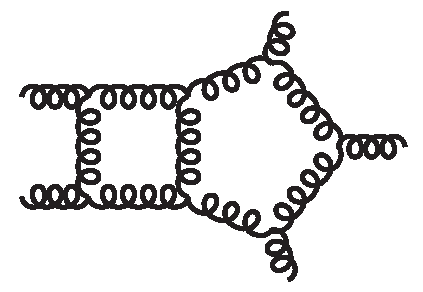
\includegraphics[scale=0.5]
    {figures/5g.pdf}};
    % 5 point masters
    \node at (5,0){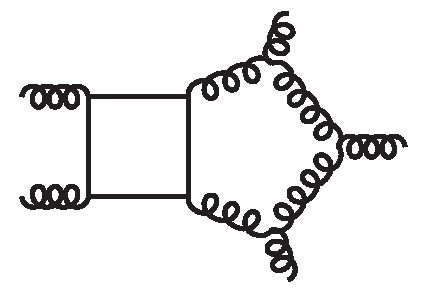
\includegraphics[scale=0.5]
    {figures/5gnf.pdf}};
    % Level 2 
    \node at (10,0){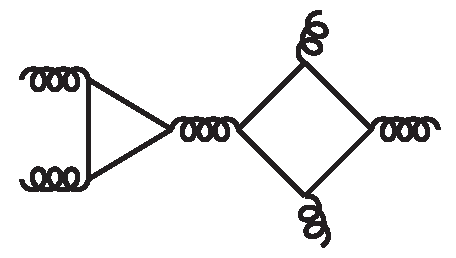
\includegraphics[scale=0.5]
    {figures/5gnf2.pdf}};
\end{tikzpicture}
\end{center} 
\caption{Representative Feynman diagrams for leading-color
$\CA^{(2)}(g,g,g,g,g)$ amplitudes, contributing at order
$N_f^0$, $N_f^1$ and $N_f^2$.}
\label{fig_parents5g}
\end{figure}

%%%%%%%%%%%%% FIGURE %%%%%%%%%%%%%%%%%%
\begin{figure}[ht]
  \begin{center}
    \begin{tikzpicture}[scale=.9]
    % 5 point masters
    \node at (0,0){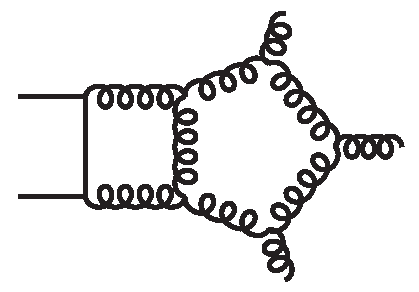
\includegraphics[scale=0.5]
    {figures/2q3g.pdf}};
    % 5 point masters
    \node at (5,0){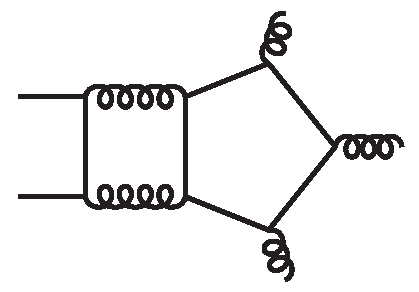
\includegraphics[scale=0.5]
    {figures/2q3gnf.pdf}};
    % Level 2 
    \node at (10,0){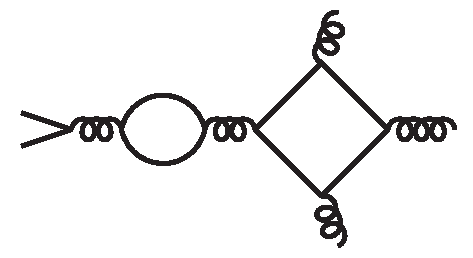
\includegraphics[scale=0.5]
    {figures/2q3gnf2.pdf}};
\end{tikzpicture}
\end{center} 
\caption{Representative Feynman diagrams for leading-color
$\CA^{(2)}(q,\bar q,g,g,g)$ amplitudes, 
contributing at order
 $N_f^0$, $N_f^1$ and $N_f^2$.}
\label{fig_parents2q3g}
\end{figure}

%%%%%%%%%%%%% FIGURE %%%%%%%%%%%%%%%%%%
\begin{figure}[ht]
  \begin{center}
    \begin{tikzpicture}[scale=.9]
    % 5 point masters
    \node at (0,0){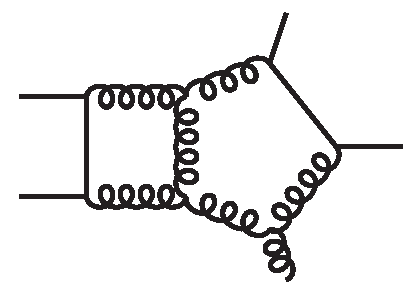
\includegraphics[scale=0.5]
    {figures/4q1g.pdf}};
    % 5 point masters
    \node at (5,.4){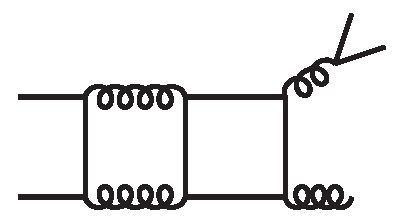
\includegraphics[scale=0.5]
    {figures/4q1gnf.pdf}};
    % Level 2 
    \node at (10,.4){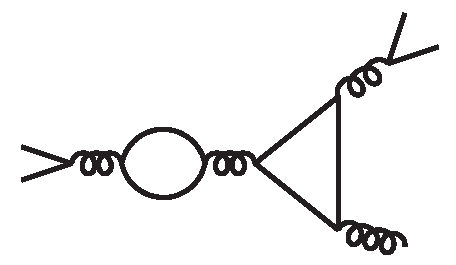
\includegraphics[scale=0.5]
    {figures/4q1gnf2.pdf}};
\end{tikzpicture}
\end{center} 
\caption{Representative Feynman diagrams for leading-color
$\CA^{(2)}(q,\bar q,Q,\bar Q,g)$ amplitudes, 
contributing at order
$N_f^0$, $N_f^1$ and $N_f^2$.}
\label{fig_parents4q1g}
\end{figure}


\subsection{Color Structure}
\label{5parton:sec:color_structures}
We decompose all amplitudes in terms of color structures. 
We denote the fundamental generators of the
$SU(\NC)$-group by $(T^a)^{\;\bar{\jmath}}_{i}$, where the
adjoint index $a$ runs over $\NC^2-1$ values and the 
(anti-) fundamental indices $i$  ($\bar \jmath$)
run over $\NC$ values. The fundamental generators are normalized
as $ \Tr(T^a T^b) = \delta^{ab}$. One can then consider the color decomposition of
each process as
%
\begin{align}
  \begin{split}
    \label{eq:ColorDecG}
    A(1_g, 2_g, 3_g, 4_g, 5_g) \big\vert_{\textrm{leading color}} = &
    \sum_{\sigma\in S_5/Z_5} \Tr\left(
    T^{a_{\sigma(1)}} T^{a_{\sigma(2)}} 
    T^{a_{\sigma(3)}} T^{a_{\sigma(4)}} T^{a_{\sigma(5)}} \right)\\
    &\times \CA({\sigma(1)}_g, {\sigma(2)}_g, {\sigma(3)}_g, {\sigma(4)}_g, {\sigma(5)}_g)\,, 
  \end{split} \\
  \begin{split}
    \label{eq:ColorDec2Q}
    A(1_q, 2_{\bar{q}}, 3_g, 4_g, 5_g) \big\vert_{\textrm{leading color}} 
    = & \sum_{\sigma\in S_3} 
    \left( T^{a_{\sigma(3)}} T^{a_{\sigma(4)}} T^{a_{\sigma(5)}} \right)^{\;\bar{\imath}_2}_{i_1} \\
    & \times\CA(1_q,2_{\bar{q}},\sigma(3)_g,\sigma(4)_g,\sigma(5)_g)\,,
  \end{split}\\
  \begin{split}
    \label{eq:ColorDec4Q}
    A(1_q, 2_{\bar{q}}, 3_Q, 4_{\bar{Q}}, 5_g)
    \big\vert_{\textrm{leading color}} 
    = & 
  %
    \,(T^{a_5})^{\;\bar{\imath}_{2}}_{i_{3}} \delta^{\;\bar{\imath}_{4}}_{i_{1}}\;
  %
    \CA(1_{q}, 2_{\bar{q}}, 5_g, 3_{Q}, 4_{\bar{Q}}) \,\,+  \\
  %
    & \,(T^{a_5})^{\;\bar{\imath}_{4}}_{i_{1}} \delta^{\;\bar{\imath}_{2}}_{i_{3}}\;
  %
    \CA(1_{q},2_{\bar{q}},3_{Q},4_{\bar{Q}},5_g) \,,
  \end{split}
\end{align}
where $S_n$ denotes all permutations of $n$ indices and 
$S_n/Z_n$ all non-cyclic permutations of $n$ indices. 
We write the particle type explicitly as a subscript, and all
remaining properties of each particle (momentum, helicity, 
etc.\@) are implicit. 

The $\CA$ in \cref{eq:ColorDecG,eq:ColorDec2Q,eq:ColorDec4Q} are
called partial amplitudes. For each of the amplitudes considered, all
partial amplitudes can be related to the others by exchanging external
legs, so only one partial amplitude is independent. These are expanded in a perturbative
expansion,
\begin{equation}
    \label{eq:partials} 
    \CA
    = g^{3}_0 \left(
        \CA^{(0)}
      + \frac{\alpha_0}{4\pi}\NC \CA^{(1)}
      + \left(\frac{\alpha_0}{4\pi}\right)^2\NC^2  \CA^{(2)} 
      + \mathcal{O}(\alpha_0^3)
      \right),
\end{equation}
where $\alpha_0=g_0^2/(4\pi)$ is the bare QCD coupling and 
$\CA^{(k)}$ denotes a $k$-loop partial amplitude. Each 
$\CA^{(k)}$ can be further expanded as a series in powers of 
$N_f/N_c$,
\begin{align}
  \label{eq:nfdecomposition} 
  \begin{split}
  \CA^{(1)} &= \CA^{(1)[N_f^0]} + 
  \frac{\NF}{\NC}\CA^{(1)[N_f^1]}\,, \\
  \CA^{(2)} &= \CA^{(2)[N_f^0]} +
  \frac{\NF}{\NC}\CA^{(2)[N_f^1]} +
  \left(\frac{\NF}{\NC}\right)^2\CA^{(2)[N_f^2]}\,.
  \end{split} 
\end{align}
We compute the coefficients $\CA^{(k)[N_f^l]}$, with $0\leq l\leq
k\leq2$, where only planar diagrams contribute as we work in the
leading-color approximation. In figs.~\ref{fig_parents5g},
\ref{fig_parents2q3g} and \ref{fig_parents4q1g} we give representative
diagrams for each of these contributions.


\subsection{Divergence Structure}
\label{sec:IR}

\subsubsection{Renormalization}

We perform renormalization of the QCD coupling in the 
$\overline{\text{MS}}$ scheme. It is implemented by replacing 
the bare coupling by the renormalized one, denoted $\alpha_s$, 
in eq.~\eqref{eq:partials}.
The bare and renormalized couplings are related through
\begin{equation}\label{eq:renormCoupling}
    \alpha_0\mu_0^{2\epsilon}S_{\epsilon}
  =\alpha_s\mu^{2\epsilon}\left(
  1-\frac{\beta_0}{\epsilon}\frac{\alpha_s}{4\pi}
  +\left(\frac{\beta_0^2}{\epsilon^2}-\frac{\beta_1}{\epsilon}\right)
  \left(\frac{\alpha_s}{4\pi}\right)^2+\mathcal{O}
  \left(\alpha_s^3\right)\right),
\end{equation}
where $S_\epsilon=(4\pi)^{\eps}e^{-\eps\gamma_E}$, with
$\gamma_E=-\Gamma'(1)$ the Euler-Mascheroni constant.
$\mu_0^2$ is the scale introduced in dimensional regularization
to keep the coupling dimensionless in the QCD Lagrangian, 
and $\mu^2$ is the renormalization scale. In the following, we
set $\mu_0^2=\mu^2=1$. The leading-color coefficients of the QCD
$\beta$-function are
\begin{equation}
  \beta_0=\frac{\NC}{3} \left( 11 - 2\frac{N_f}{\NC}
  \right),\qquad
  \beta_1=\frac{\NC^2}{3} \left( 17 - \frac{13}{2} \frac{N_f}{\NC} \right).
\end{equation}
The perturbative expansion of the renormalized amplitude is
\begin{equation}\label{eq:renormAmp}
  \mathcal{A}_R = S_\epsilon^{-\frac{\lambda}{2}}
  g_s^\lambda\left(
  \mathcal{A}_R^{(0)}
  +\frac{\alpha_s}{4\pi}\NC\,\mathcal{A}_R^{(1)}
  +\left(\frac{\alpha_s}{4\pi}\right)^2\NC^2\mathcal{A}_R^{(2)}
  +\mathcal{O}(\alpha_s^3)
  \right),
\end{equation}
where $\lambda$ is the power of $g_0$ in the tree amplitude, 
with $\alpha_0=g_0^2/(4\pi)$ and similarly for $\alpha_s$.
For four-parton amplitudes $\lambda=2$, and for five-parton 
amplitudes $\lambda=3$.
The renormalized amplitudes $\mathcal{A}_R^{(i)}$ are related 
to the bare amplitudes $\mathcal{A}^{(i)}$ as follows:
\begin{align}
  \begin{split}
    \label{eq:twoLoopUnRenorm}
    &\mathcal{A}_R^{(0)}=\mathcal{A}^{(0)}, \\
    & \mathcal{A}_R^{(1)}=S_{\epsilon}^{-1}\mathcal{A}^{(1)}
    -\frac{\lambda}{2\epsilon}\frac{\beta_0}{\NC}
    \mathcal{A}^{(0)}\,,\\
    &\mathcal{A}_R^{(2)}=
    S_{\epsilon}^{-2}\mathcal{A}^{(2)}
    -\frac{\lambda+2}{2\epsilon}\frac{\beta_0}{\NC}S_{\epsilon}^
    {-1}
    \mathcal{A}^{(1)}
    +\left(\frac{\lambda(\lambda+2)}{8\epsilon^2}\left(\frac{\beta_0}
    {\NC}\right)^2
    -\frac{\lambda}{2\epsilon}\frac{\beta_1}{\NC^2}\right)
    \mathcal{A}^{
    (0)}\,.
  \end{split}
\end{align}



\subsubsection{Infrared Behavior}

The poles of renormalized amplitudes are of infrared origin and
can be predicted from the previous orders in the perturbative 
expansion 
\cite{Catani:1998bh,Sterman:2002qn,Becher:2009cu,Gardi:2009qi}:
\begin{align}
  \begin{split}\label{eq:catani}
    A_R^{(1)}&=\mathbf{I}^{(1)}_{[n]}(\epsilon)
    A_R^{(0)}+\mathcal{O}
    (\epsilon^0)\,,\\
    A_R^{(2)}&=\mathbf{I}^{(2)}_{[n]}(\epsilon)A_R^{(0)}+\mathbf{I}^{(1)}_{[n]}(\epsilon)
    A_R^{(1)}+\mathcal{O}(\epsilon^0)\,,
  \end{split}
\end{align}
with the operators $\mathbf{I}^{(1)}_{[n]}$ and
$\mathbf{I}^{(2)}_{[n]}$ depending on the number and the type of
the scattering particles. This dependence is denoted by the 
subscript $[n]$.
For amplitudes in the leading-color approximation and for which
all quark lines have distinct flavor, the operators
$\mathbf{I}^{(1)}_{[n]}$ and $\mathbf{I}^{(2)}_{[n]}$ are 
diagonal in color space and can be written in a very compact
form. The operator $\mathbf{I}^{(1)}_{[n]}$ is given by
%
\begin{equation}
  \mathbf{I}^{(1)}_{[n]}(\eps)=-\frac{e^{\gamma_E\eps}}{\Gamma(1-\epsilon)}
  \sum_{i=1}^n\gamma_{a_i,a_{i+1}}
  \left( -s_{i,i+1}\right)^{-\epsilon}\,,
\end{equation}
with the indices defined cyclically.
The index $a_i$ denotes a type of particle with momentum $p_i$, i.e.\  in the context of our paper,
$a_i\in\{g,q,\bar q, Q, \bar Q\}$. We introduced the auxiliary symbols $\gamma_{a,b}$, 
symmetric under the exchange of indices, 
$\gamma_{a,b}=\gamma_{b,a}$, and defined according to:
\begin{align}
  \begin{split}
    \gamma_{g,g}&=\frac{1}{\epsilon^2}+\frac{1}{2\eps}
    \frac{\beta_0}{\NC}\,, \\
    \gamma_{q,Q}&=\gamma_{q,\bar Q}=
    \gamma_{\bar q, Q}=\gamma_{\bar q, \bar Q} 
    =\frac{1}{\epsilon^2}+\frac{3}{2\eps}\,,\\
    \gamma_{g,q}&=\gamma_{g,\bar q}=
    \gamma_{g,Q}=\gamma_{g,\bar Q}=
    \frac{\gamma_{g,g}+\gamma_{q,Q}}{2}\,,\\
    \gamma_{q,\bar q}&=\gamma_{Q,\bar Q}=0\,.
  \end{split}
\end{align}
The operator~$\mathbf{I}^{(2)}_{[n]}$ is
\begin{align}
  \label{eqn:Iop}
  \begin{split} 
    \mathbf{I}^{(2)}_{[n]}(\eps)=&
    -\frac{1}{2}\mathbf{I}^{(1)}_{[n]}(\eps)\mathbf{I}^{(1)}_{[n]}(\eps)
    -\frac{\beta_0}{\NC\epsilon}\mathbf{I}^{(1)}_{[n]}(\eps) + 
    \frac{e^{-\gamma_E\epsilon}\Gamma(1-2\epsilon)}
    {\Gamma(1-\epsilon)}
    \left(\frac{\beta_0}{\NC\epsilon}+K\right)
    \mathbf{I}^{(1)}_{[n]}(2\epsilon) + 
    \mathbf{H}_{[n]}(\epsilon)\,,
  \end{split}
\end{align}
where 
\begin{equation}
K=\frac{67}{9}-\frac{\pi ^2}{3}-\frac{10}{9}\frac{\NF}{\NC}\,,
\end{equation}
and $\mathbf{H}_{[n]}(\epsilon)$ is a diagonal operator at 
leading color that depends on the number of external quarks 
and gluons in the process,
\begin{align}
  \begin{split}
    \mathbf{H}_{[n]}(\epsilon)&=
    \frac{e^{\gamma_E\epsilon}}{\epsilon\Gamma(1-\epsilon)}
    \sum_{i=1}^n\left(
    \delta_{a_i,g}H_g+
    (\delta_{a_i,q}+\delta_{a_i,\bar q}
    +\delta_{a_i,Q}+\delta_{a_i,\bar Q})
    H_q
    \right)\,,
  \end{split}
\end{align}
with (see e.g.\ \cite{Bern:2003ck})
\begin{align}
  \begin{split}
    H_g&= \left(\frac{\zeta_3}{2}+\frac{5}{12}+
    \frac{11\pi^2}{144}\right)
    -\left(\frac{\pi^2}{72}+\frac{89}{108}\right)\frac{N_f}{\NC}
    +\frac{5}{27}\left(\frac{N_f}{\NC}\right)^2\,,\\
    H_q&=
    \left(\frac{7\zeta_3}{4}+\frac{409}{864}
    -\frac{11\pi^2}{96}\right)
    +\left(\frac{\pi^2}{48}-\frac{25}{216}\right)\frac{N_f}{\NC}\,.
  \end{split}
\end{align}

The poles of the bare amplitudes, as presented for example in
tables~\ref{tab:results4parton} and \ref{tab:results5parton}, can be recovered
from those of the renormalized amplitude by using
eqs.~\eqref{eq:twoLoopUnRenorm}.

\subsubsection{Finite Remainder}\label{sec:remainders}

%As we have seen above,
%the bare scattering amplitudes defined in eq.~\eqref{eq:nfdecomposition}
%have divergences of ultraviolet and infrared origin which can be predicted from lower orders in perturbation theory.
%It is convenient to remove this redundant information and define a \emph{finite remainder} that contains the new two-loop information.
%If one is concerned only about removing the divergences a definition of the remainder is not unique, so we now discuss our conventions.

We use the divergent structure of amplitudes, given by  \cref{eq:twoLoopUnRenorm,eq:catani},
to define a finite remainder $\mathcal{F}^{(2)}$ as
\begin{equation}\label{eq:remainderDef}
  \mathcal{F}^{(2)}=\mathcal{A}_R^{(2)}
  -\mathbf{I}_{[n]}^{(1)}\mathcal{A}_R^{(1)}
  -\mathbf{I}_{[n]}^{(2)}\mathcal{A}_R^{(0)}
  +\mathcal{O}(\epsilon)\,.
\end{equation}
Here we expand one-loop amplitudes $\mathcal{A}_R^{(1)}$ to order $\eps^2$ to capture the terms of order $\eps^0$
from the cancellation with the corresponding $\frac{1}{\eps^2}$ pole in the operator $\mathbf{I}_{[n]}^{(1)}$.

%This subtracts non-trivial contributions from
%the finite term of $\mathcal{A}_R^{(2)}$ that are related to 
%the lower-loop amplitudes.
%In section \ref{sec:AnalyticForm} we will obtain analytic expression for the finite remainder directly.
%If necessary one can then recover the two-loop bare amplitude $\CA^{(2)}$ by inverting
%the relations \eqref{eq:twoLoopUnRenorm}:
%\begin{align}
  %\begin{split}
    %\label{eq:ampFromRem}
    %{\mathcal{A}}^{(2)}=&\,\mathcal{F}^{(2)}+
    %S_\epsilon{\mathcal{A}}^{(1)}
    %\left(\mathbf{I}_{[n]}^{(1)}+\frac{5}{2\epsilon}
    %\frac{\beta_0}
    %{N_c}\right)\\
    %&-S_\epsilon^2 {\mathcal{A}}^{(0)}
    %\left(
    %\frac{15}{8\epsilon^2}
    %\left(\frac{\beta_0}{N_c}\right)^2+\frac{3}{2\epsilon}
    %\left(\frac{\beta_0}{N_c}\mathbf{I}_{[n]}^{(1)}-
    %\frac{\beta_1}{N_c^2}\right)-\mathbf{I}_{[n]}^{(2)}
    %\right)+\mathcal{O}(\epsilon)\,.
  %\end{split}
%\end{align}

\subsection{Construction of Cut Equations}
\label{5parton:sec:tech}

\subsubsection{Master/Surface Integrand Parametrization}

Let us first describe how do we obtain the master/surface integrand parametrization (see \cref{sec:ansatz_integrand} for details)
in the right-hand  side of \cref{eq:cut_equations} for all of the topologies appearing in five-parton amplitudes (see \cref{fig:PropagatorStructures}).
We employ the implementation of computational algebraic geometry methods in the package \textsc{Singular} \cite{DGPS}
to solve the non-doubling conditions \eqref{eq:non_doubling_ibp_vectors},
and find the corresponding unitarity-compatible IBP vectors.
Some technical details of our setup can be found in \cite{Abreu:2017hqn}.
We then use these vectors to generated an overcomplete set of surface terms by multiplying
them with all monomials in ISPs, and inserting them into \cref{eq:ibps}.
Finally, we identify the spanning set with imposed on-shell conditions, on a randomly chosen numerical 
point.


The fast evaluation of surface terms is crucial in our approach.
To this end, we employ the following optimizations:
\begin{itemize}
  \item We represent the analytic expressions for the surface terms
    as the linear combinations of components of IBP-generating vectors, multiplied by derivatives of the ISPs,
    plus the divergences of the IBP-vectors (multiplied by ISPs). 
    Effectively, this implements the caching of common sub-expressions, which would be found in the full expression for the corresponding surface term.
  \item We optimize the expressions with the help of the command \texttt{\#optimize} from \texttt{FORM} \cite{Vermaseren:2000nd},
    which implements an extensive set of methods to bring the polynomials into the most efficient computational form.
\end{itemize}

%%%%%%%%%%%%% FIGURE %%%%%%%%%%%%%%%%%%
\begin{figure}[ht] 
  \begin{center}
    \begin{tikzpicture}[scale=1.1]
    % 5 point masters
      \node at (2.5,0){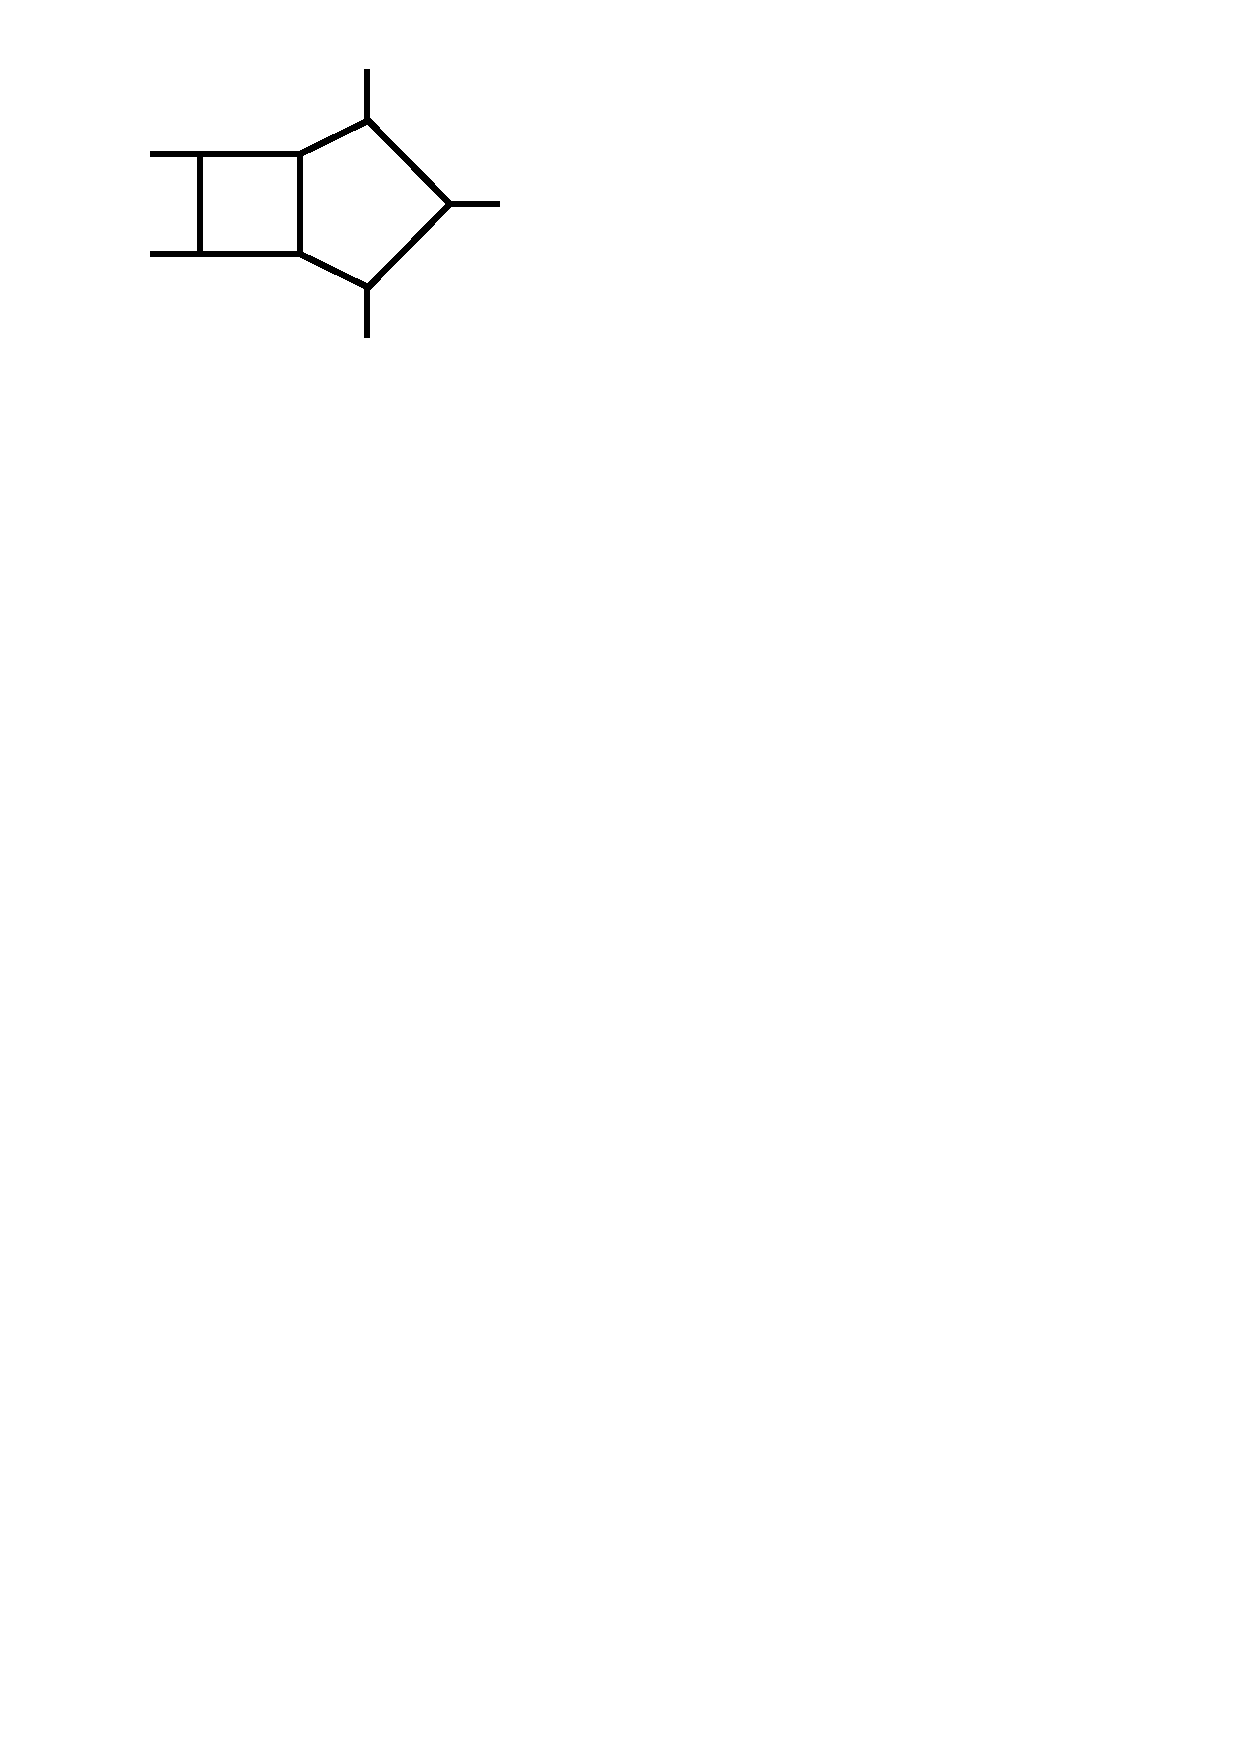
\includegraphics[scale=0.4]{figures/topologies/BoxPentagon}};
      \node at (5,0){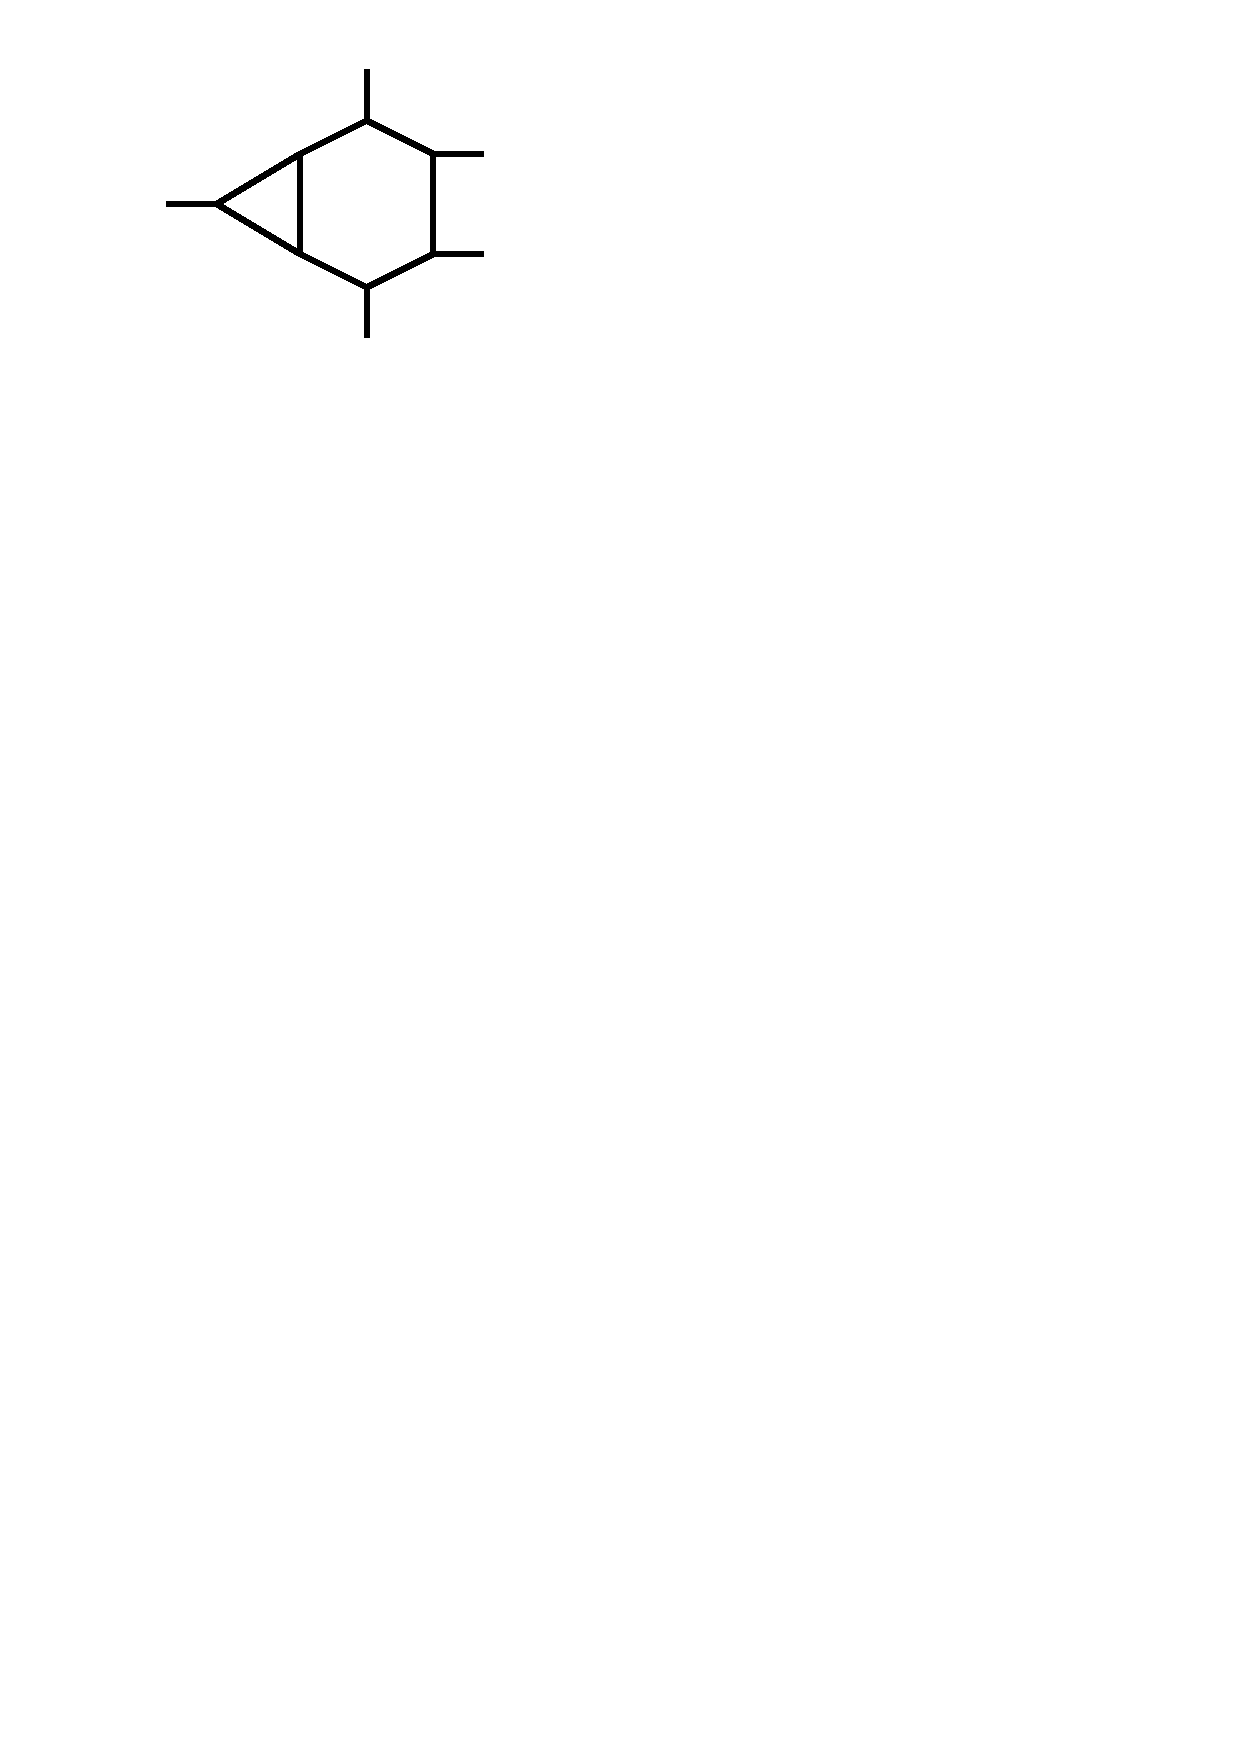
\includegraphics[scale=0.4]{figures/topologies/TriangleHexagonRed1}};
      \node at (7.5,0){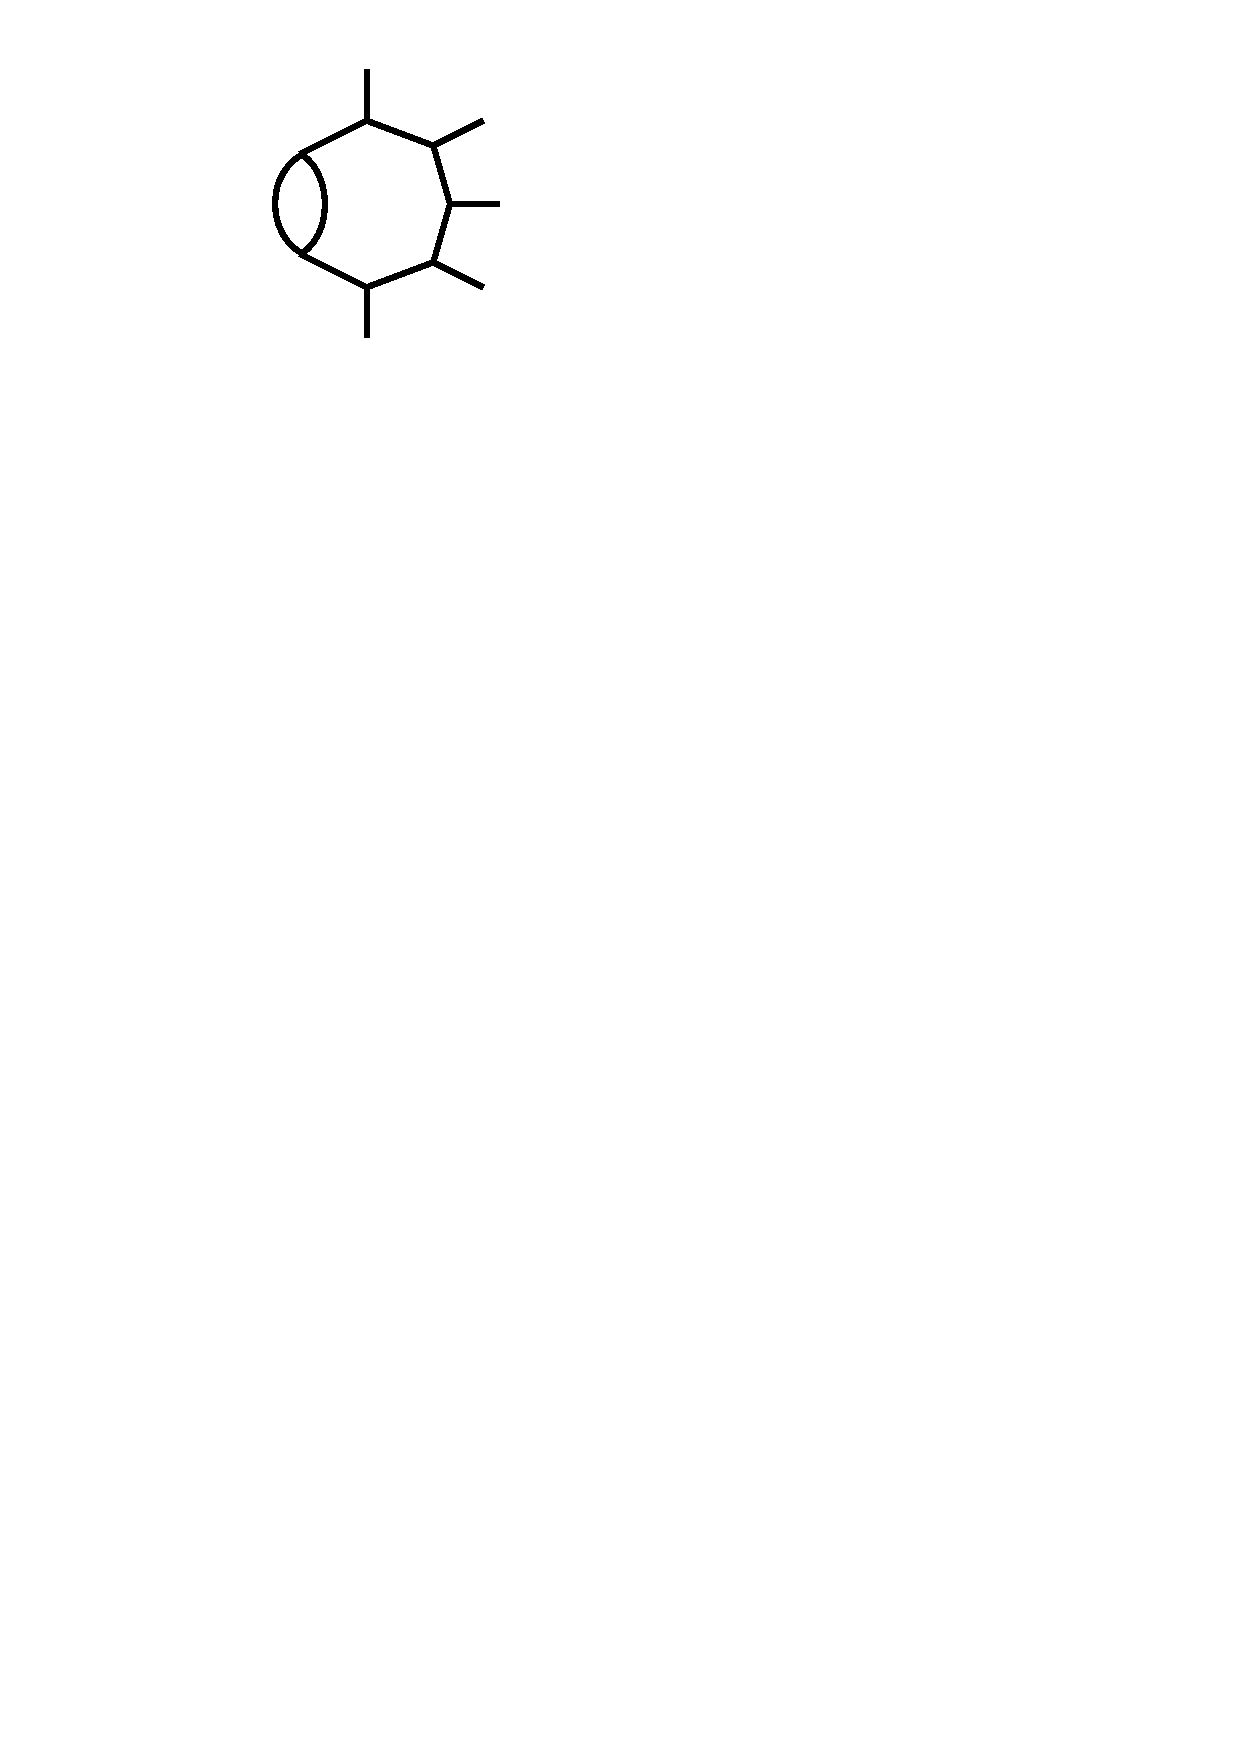
\includegraphics[scale=0.4]{figures/topologies/BubbleHeptagon}};
    % Level 2 
      \node at
      (0,-1.9){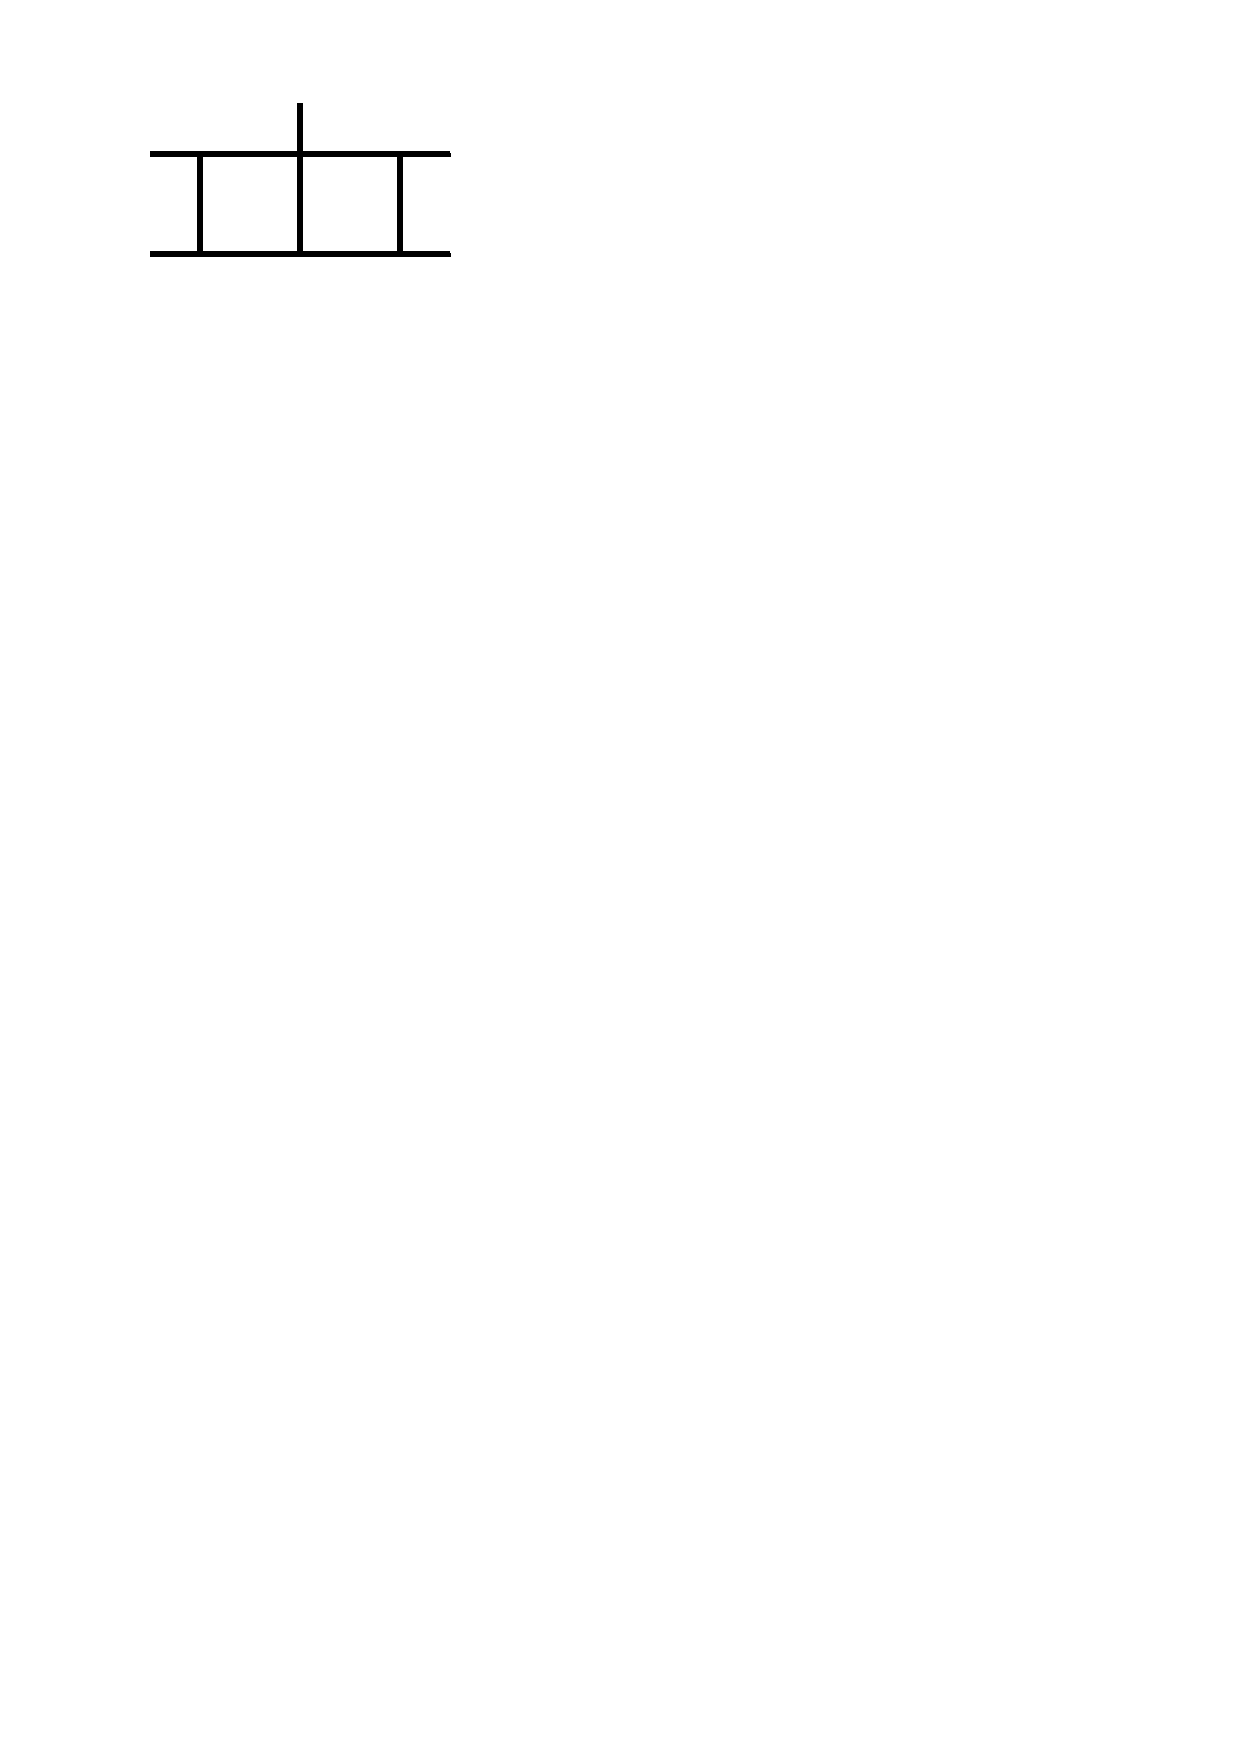
\includegraphics[scale=0.4]{figures/topologies/BoxBoxSG}};
      \node at
      (2.5,-2.0){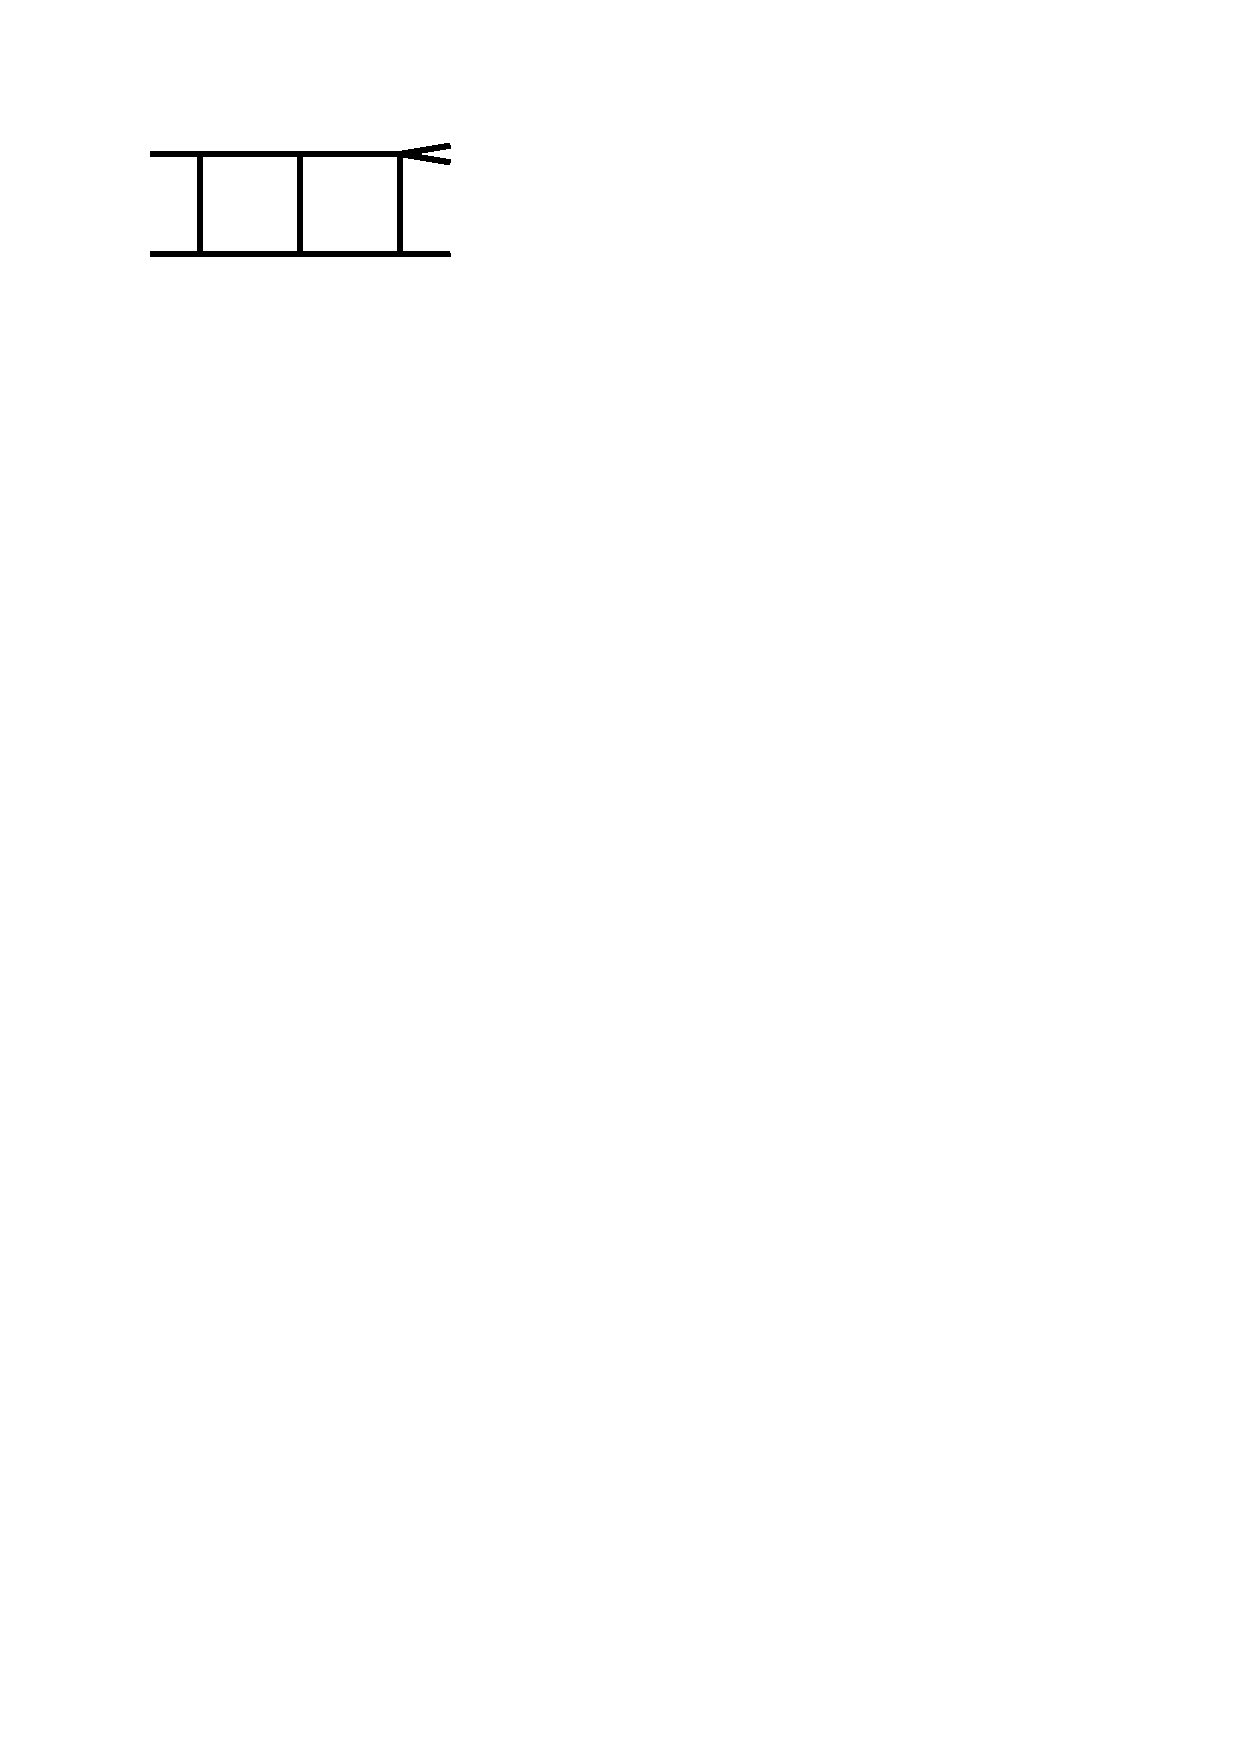
\includegraphics[scale=0.4]{figures/topologies/BoxBox}};
      \node at
      (5,-2.0){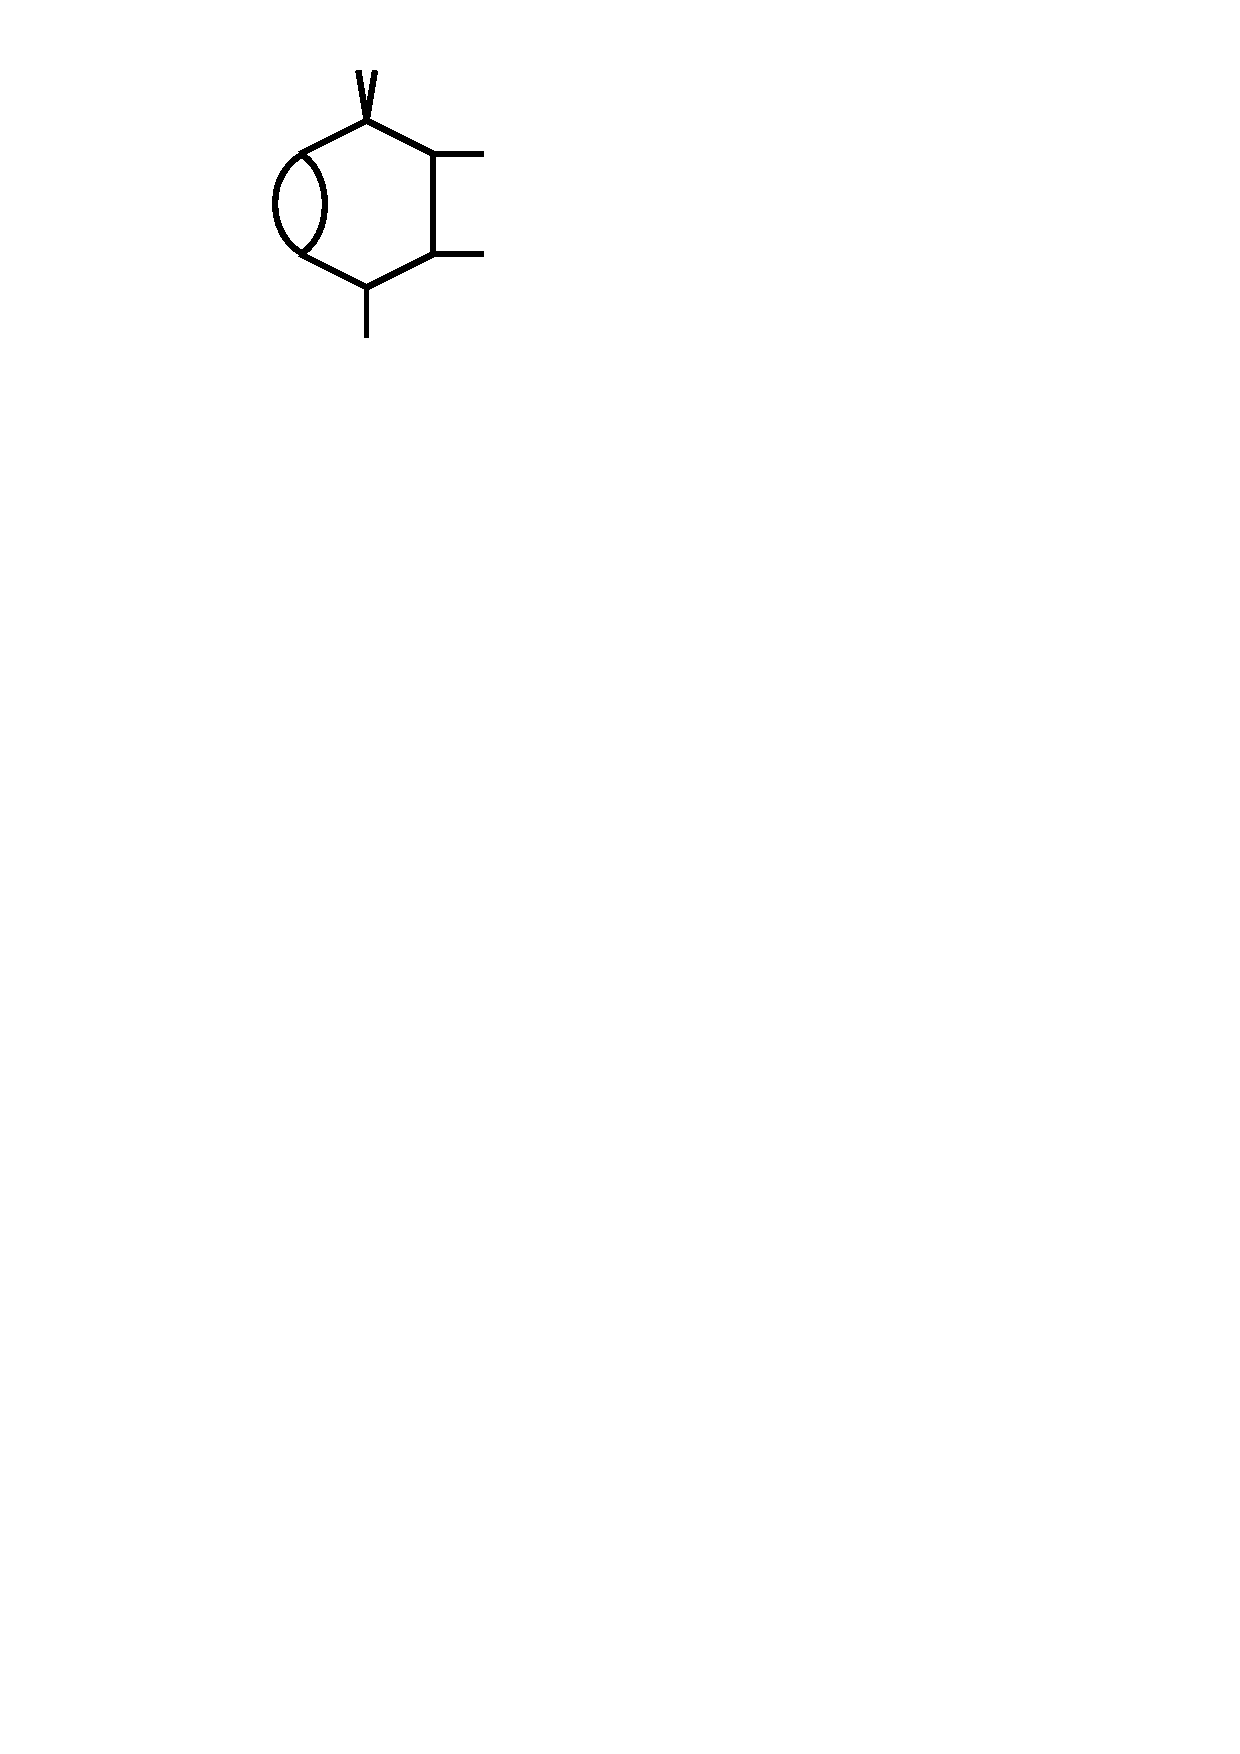
\includegraphics[scale=0.35]{figures/topologies/BubbleHexagonRed1}};
      \node at
      (7.5,-2.0){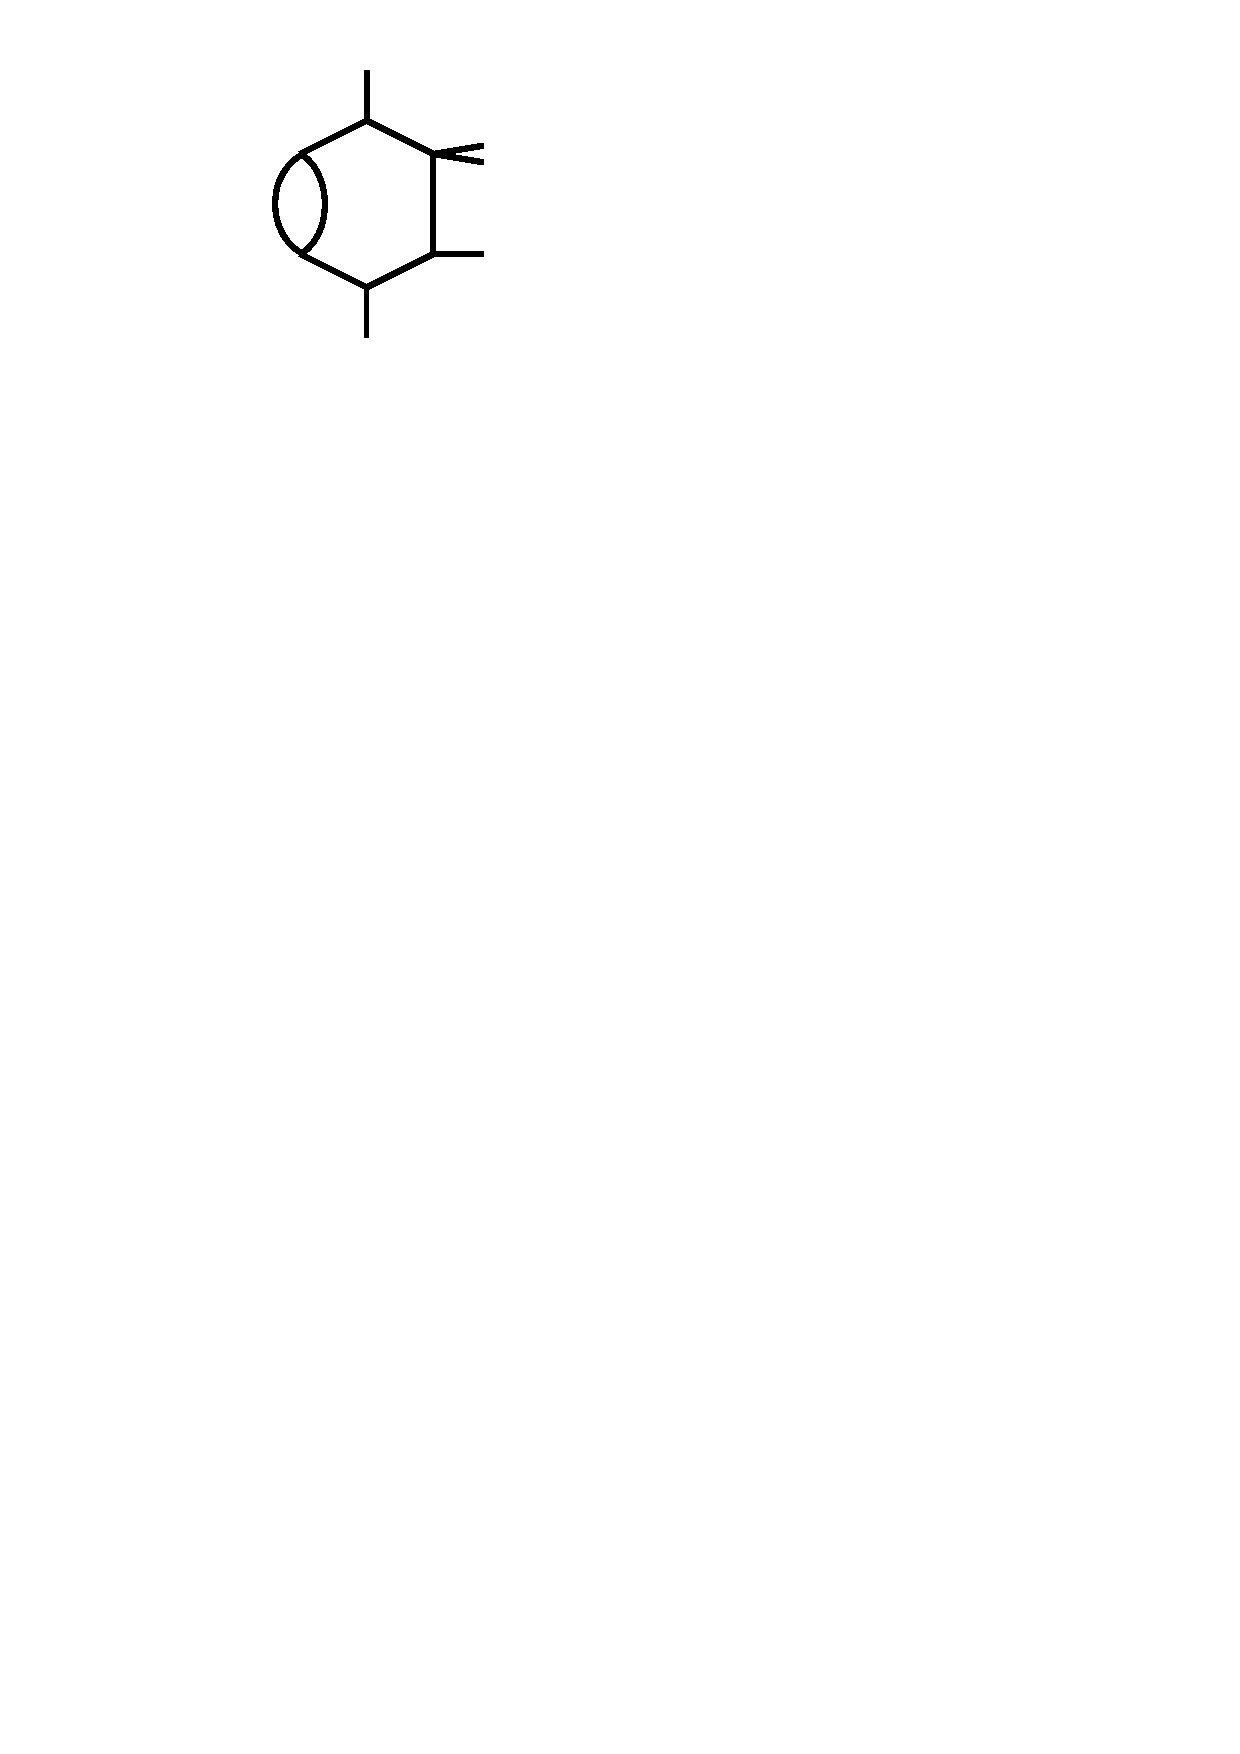
\includegraphics[scale=0.35]{figures/topologies/BubbleHexagonRed2}};
      \node at
      (10,-2.0){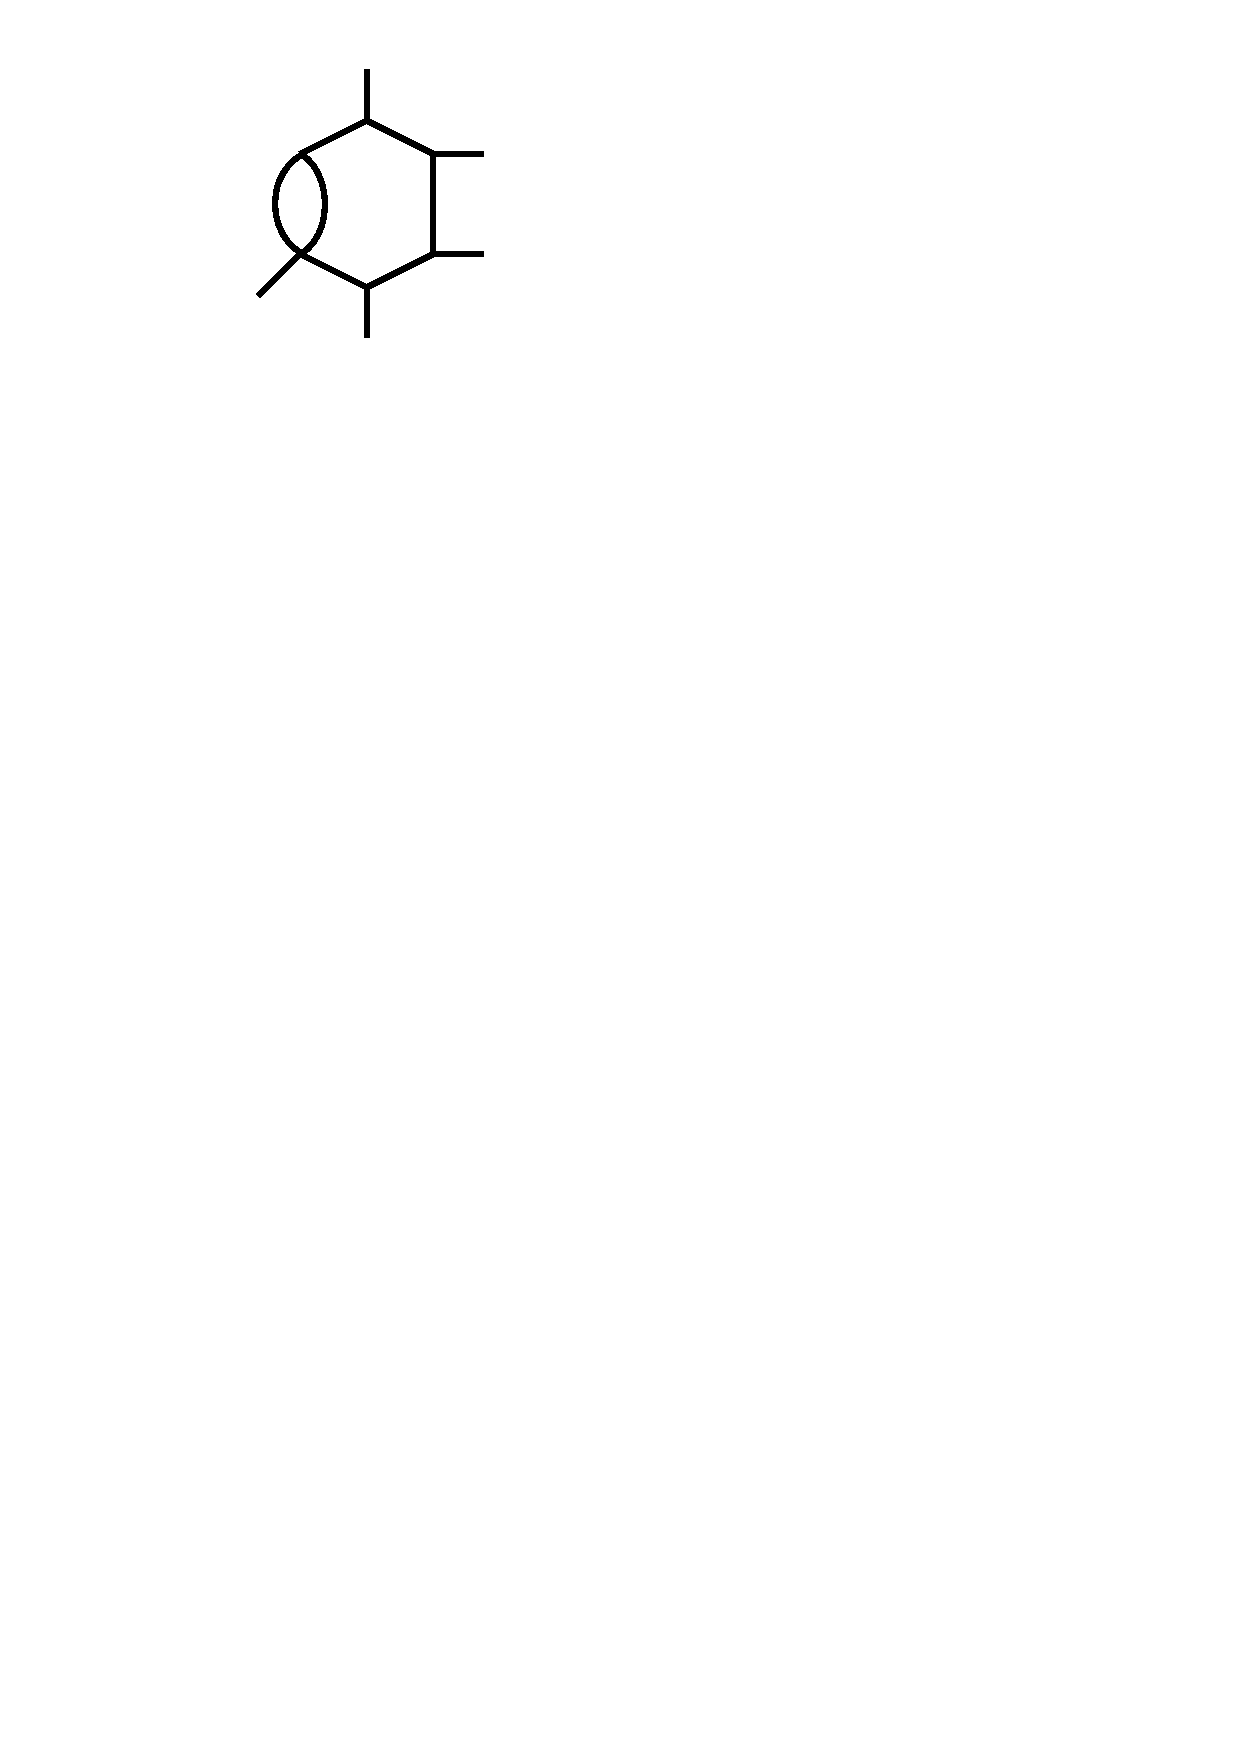
\includegraphics[scale=0.35]{figures/topologies/BubbleHexagonRed3}};
    %
      \node at
      (0,-3.6){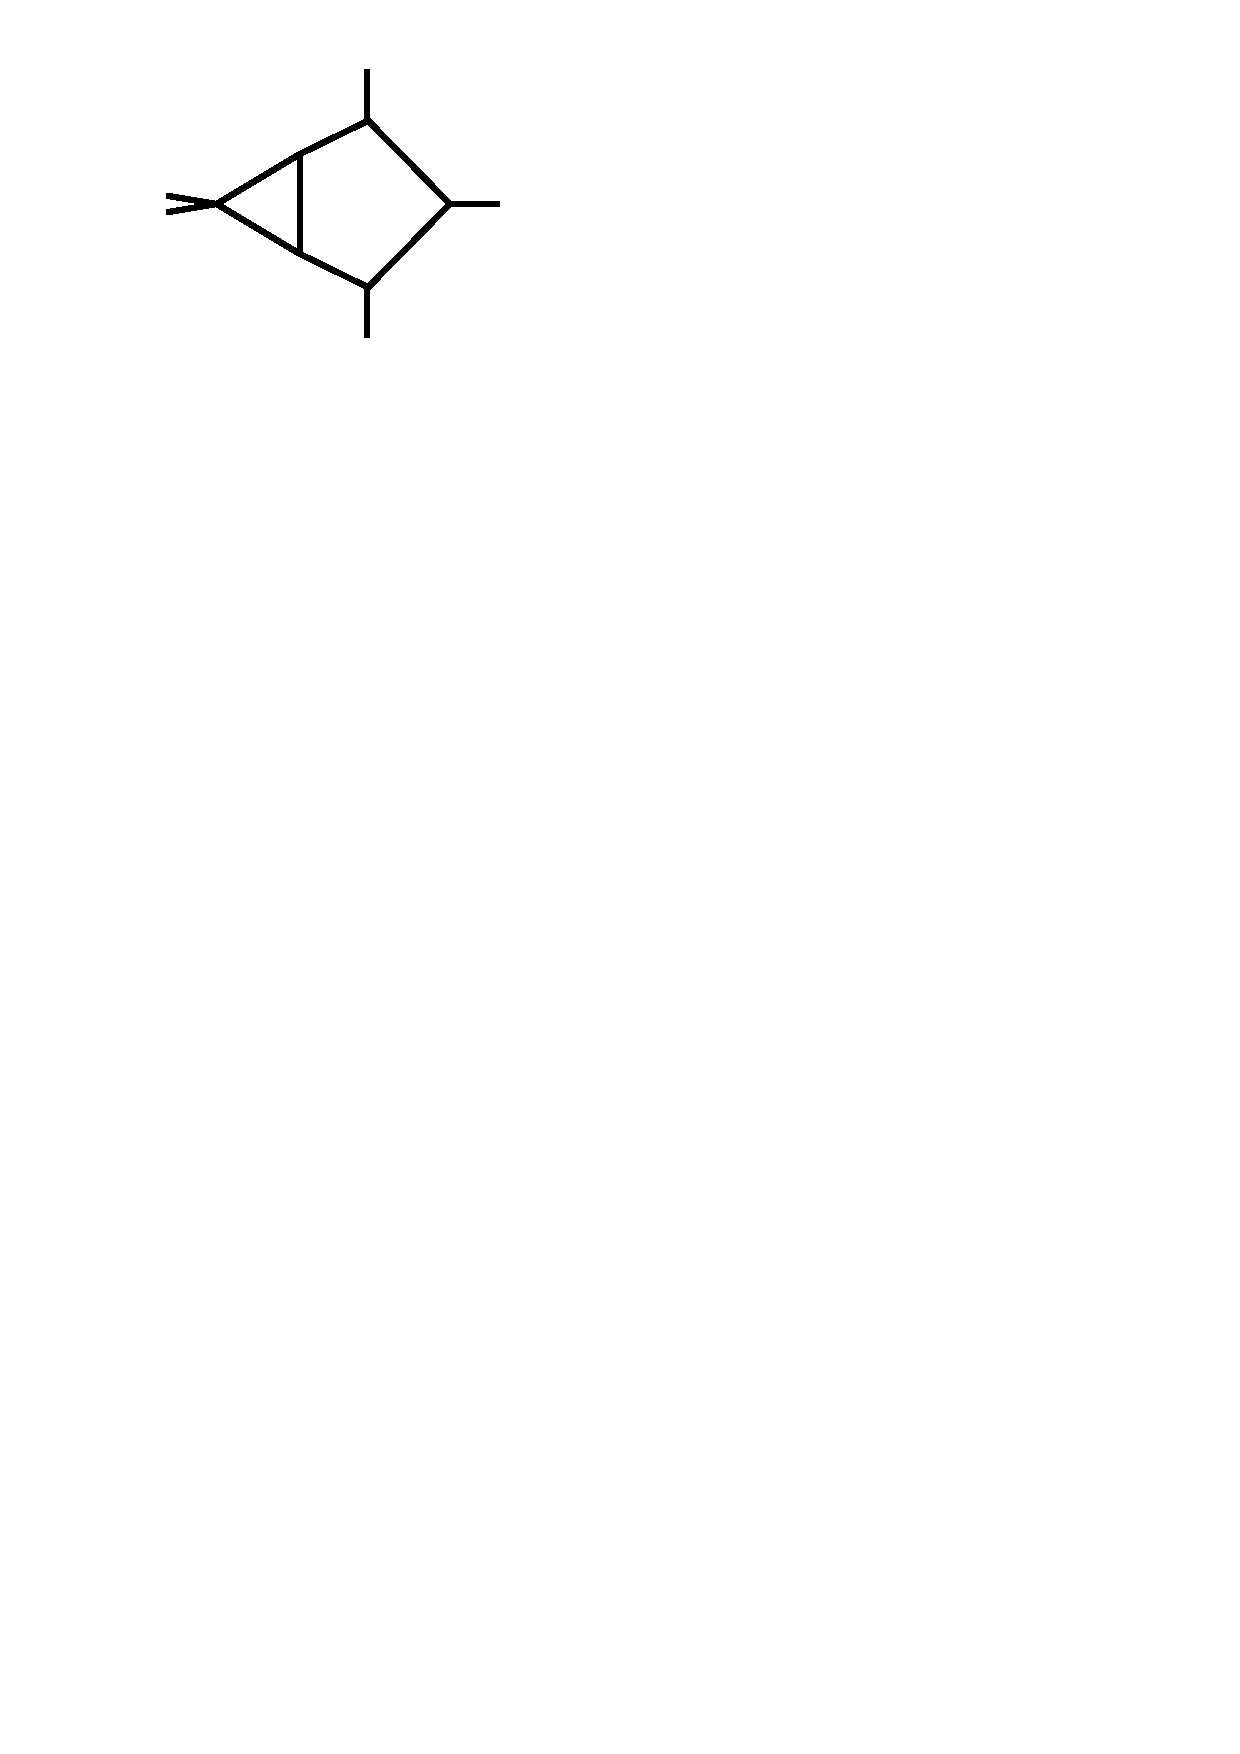
\includegraphics[scale=0.35]{figures/topologies/TrianglePentagonRed1}};
      \node at
      (2.5,-3.6){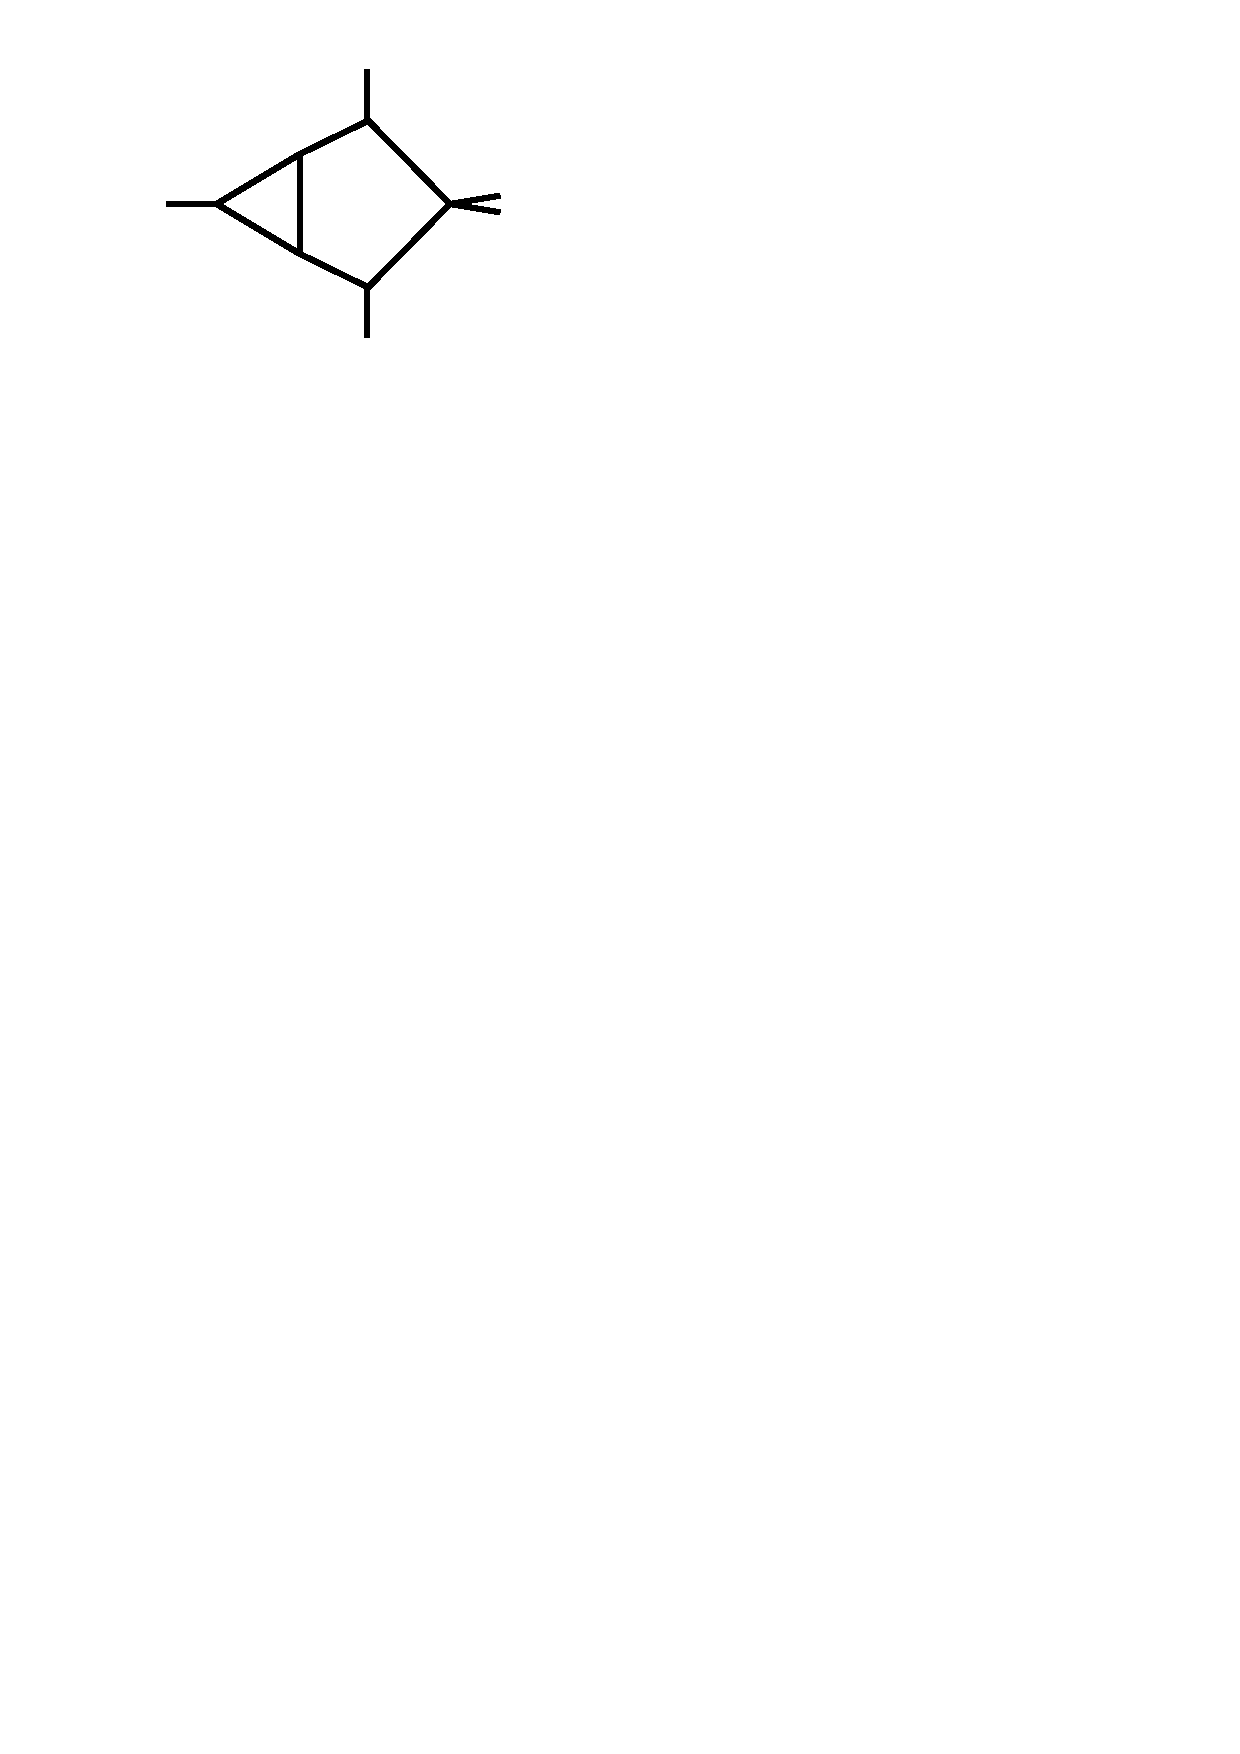
\includegraphics[scale=0.35]{figures/topologies/TrianglePentagonRed2}};
      \node at
      (5,-3.6){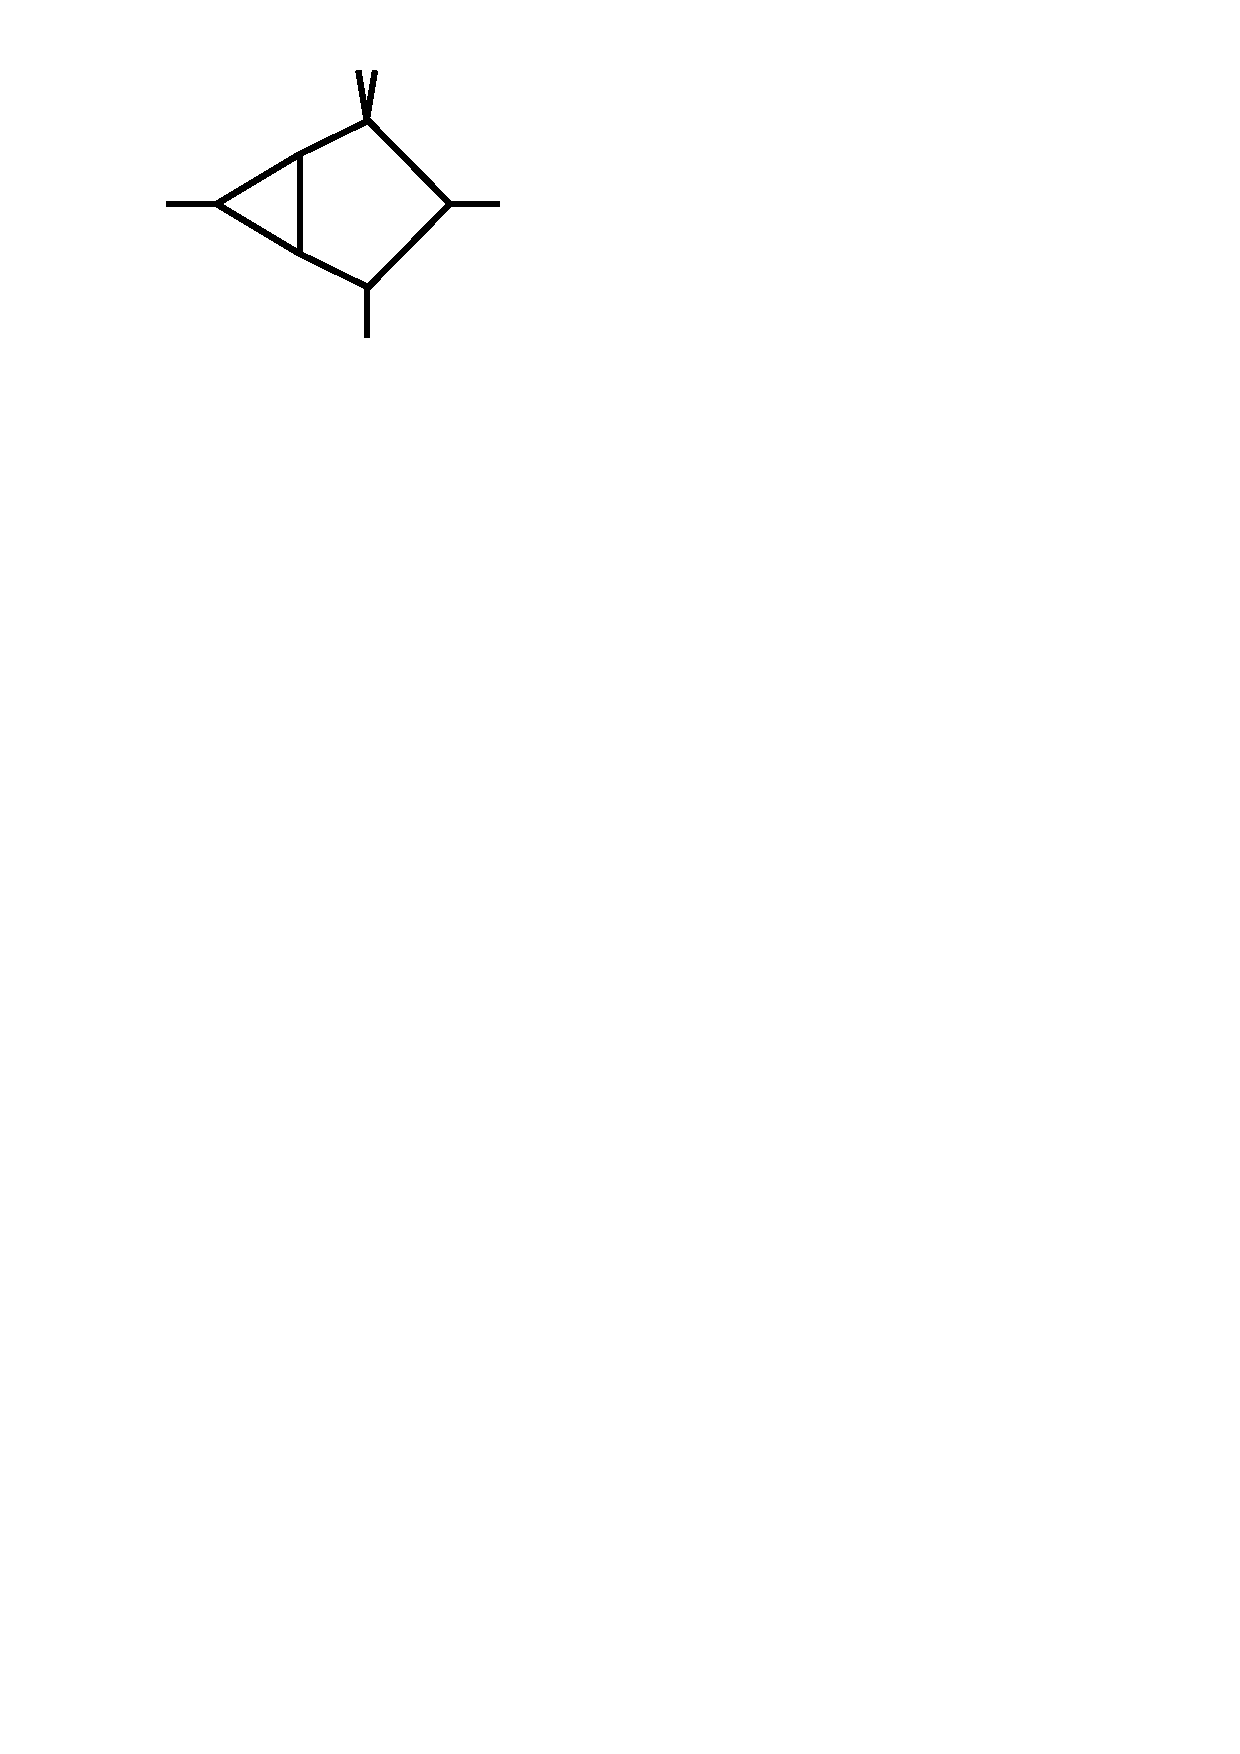
\includegraphics[scale=0.35]{figures/topologies/TrianglePentagonRed3}};
      \node at
      (7.5,-3.6){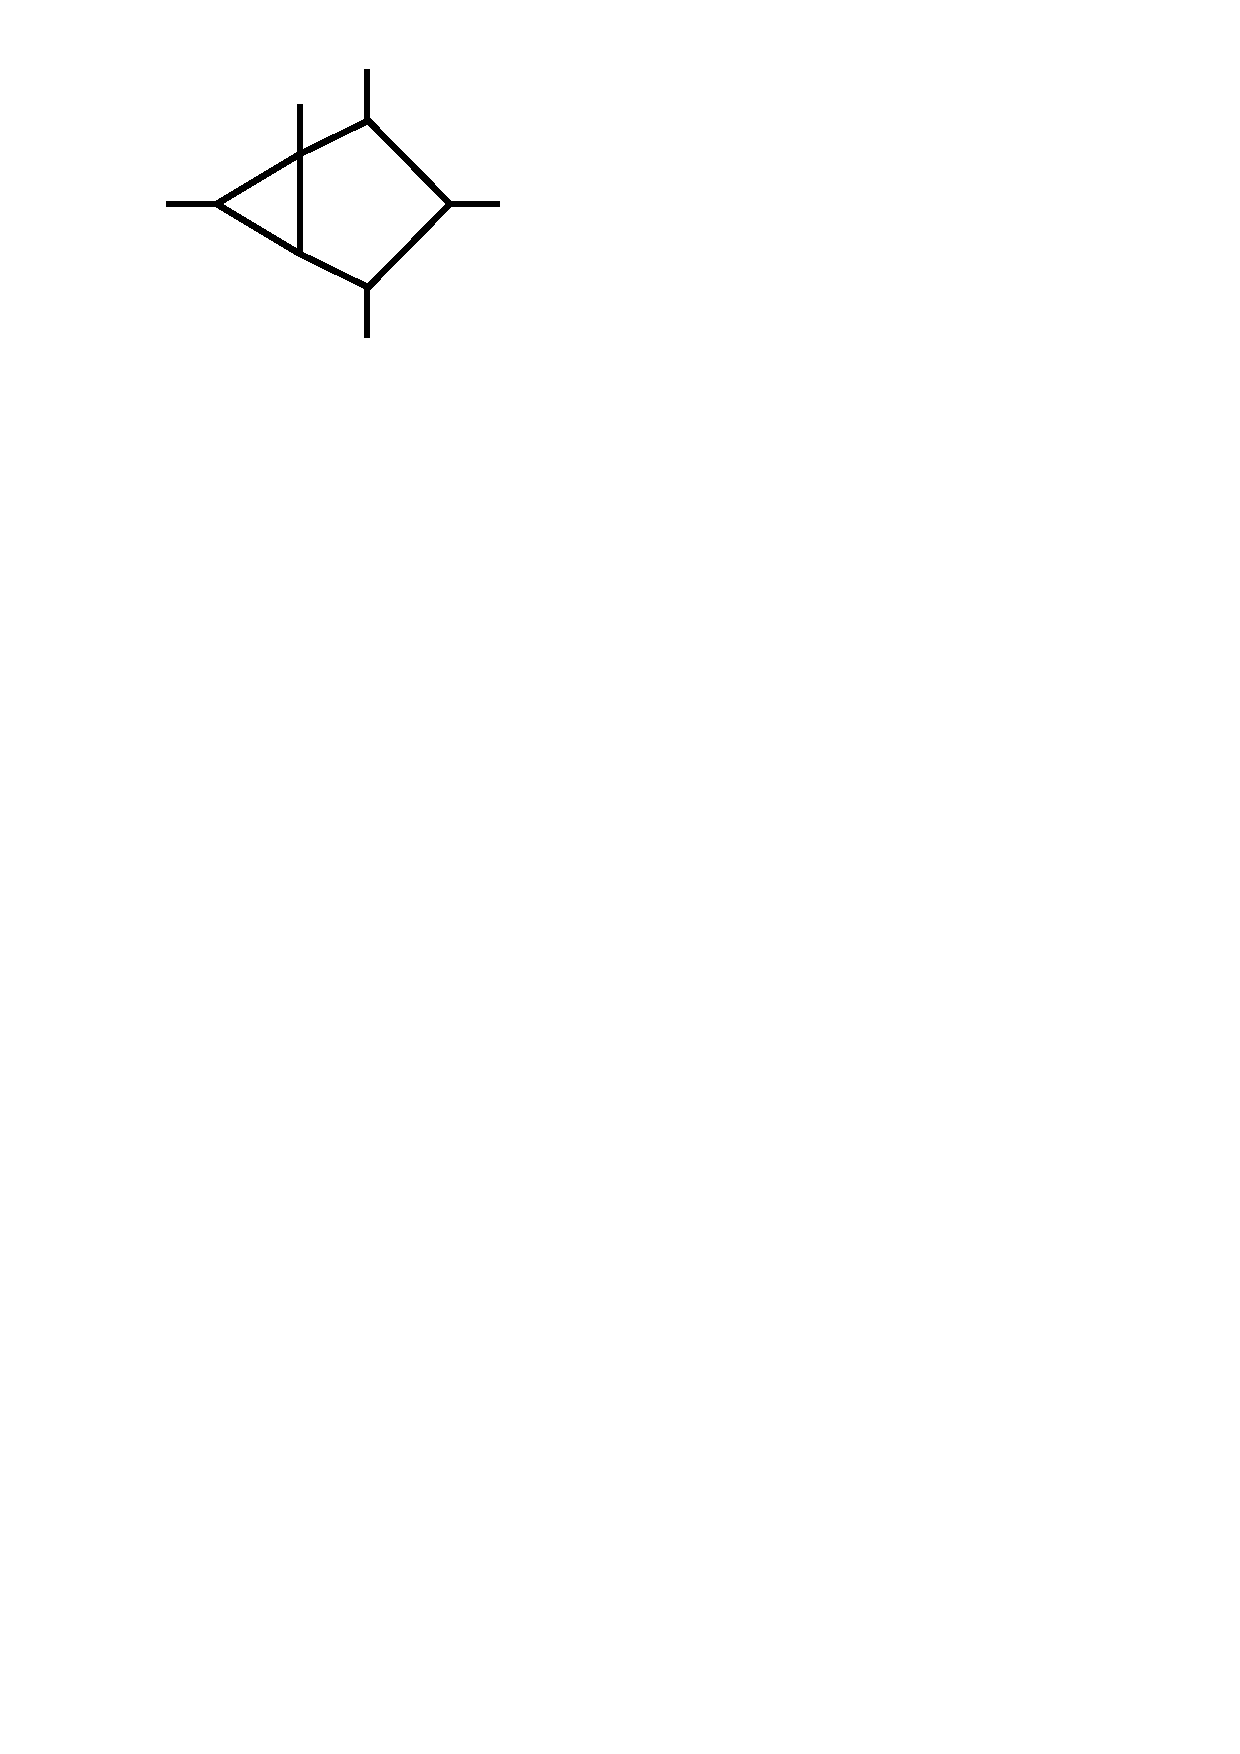
\includegraphics[scale=0.35]{figures/topologies/TrianglePentagonRed4}};
      \node at
      (10,-3.6){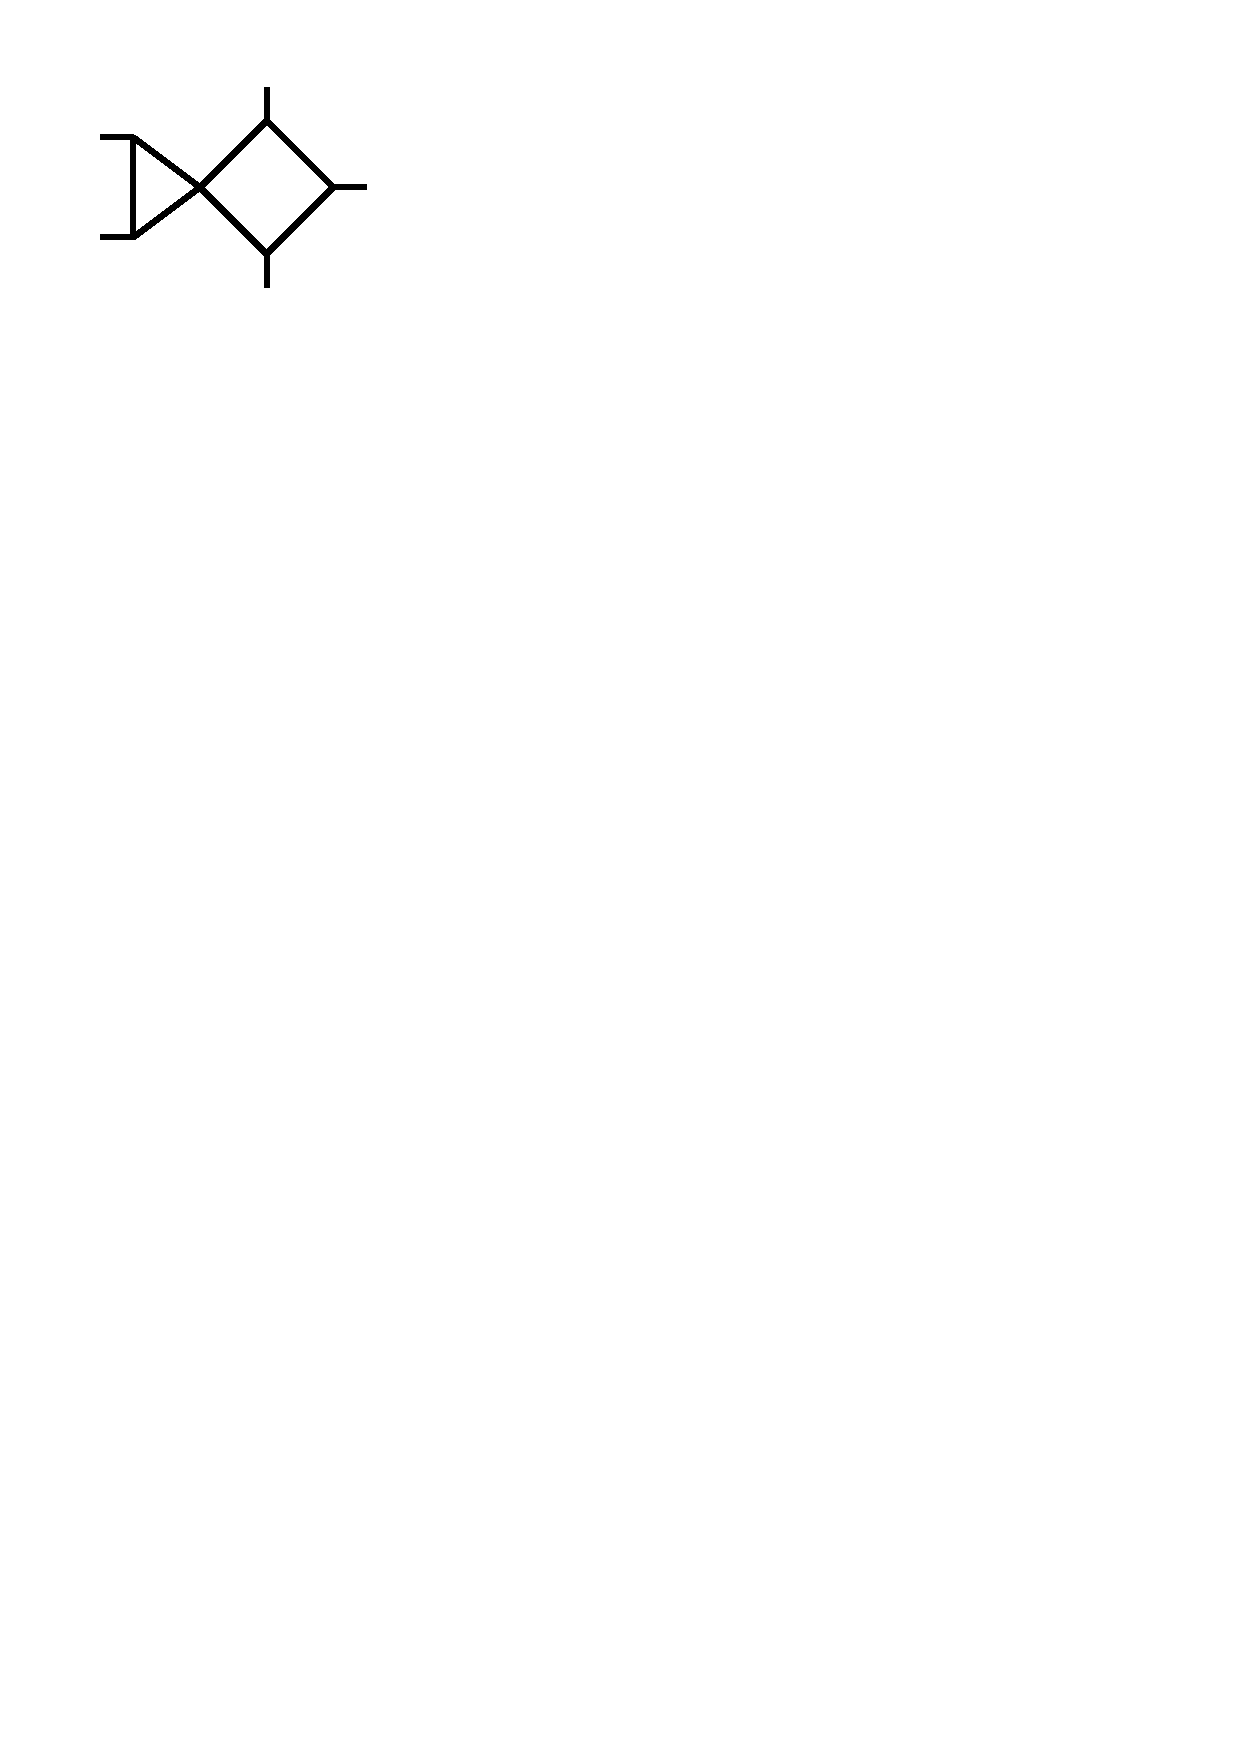
\includegraphics[scale=0.4]{figures/topologies/BoxTriangle1LS}};
    % Level 3
      \node at
      (0,-5.5){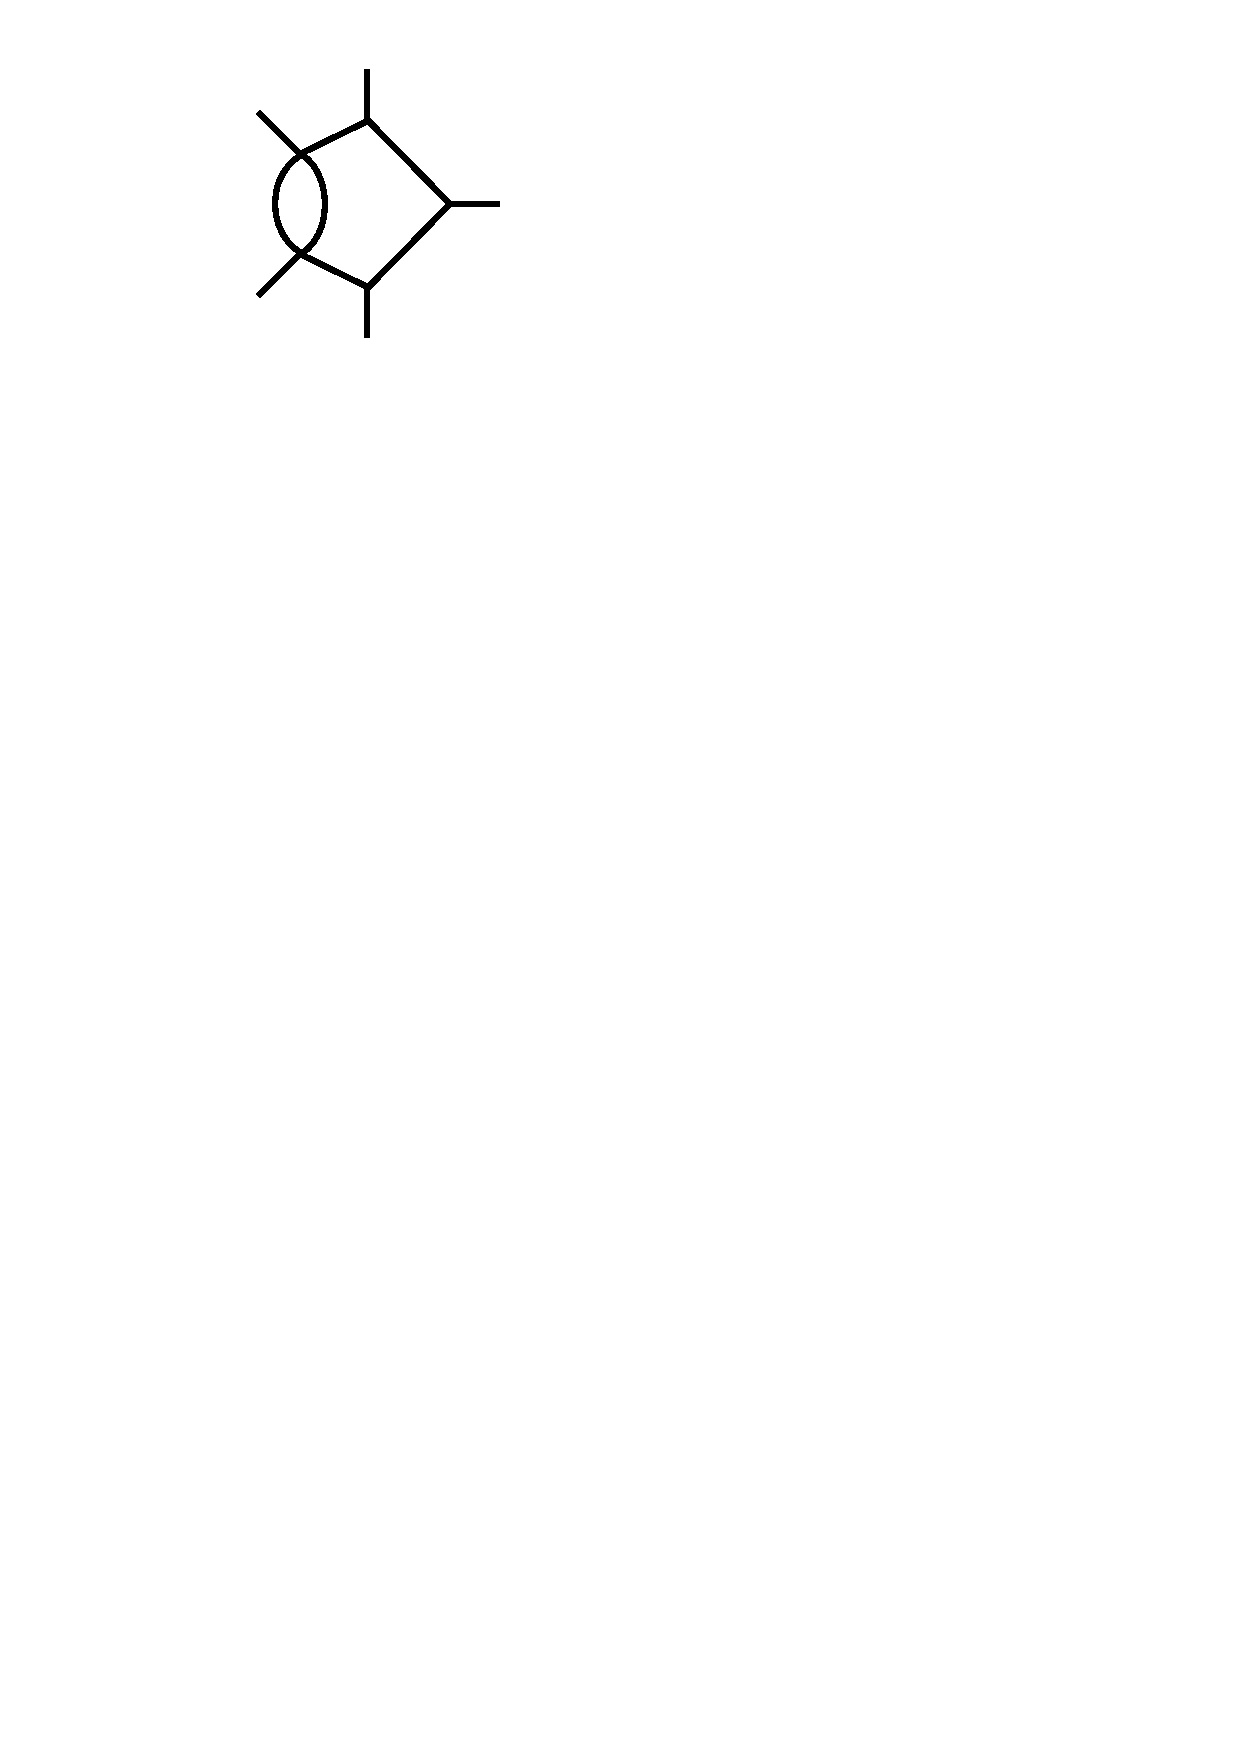
\includegraphics[scale=0.35]{figures/topologies/BubblePentagonG}};
      \node at
      (2,-5.5){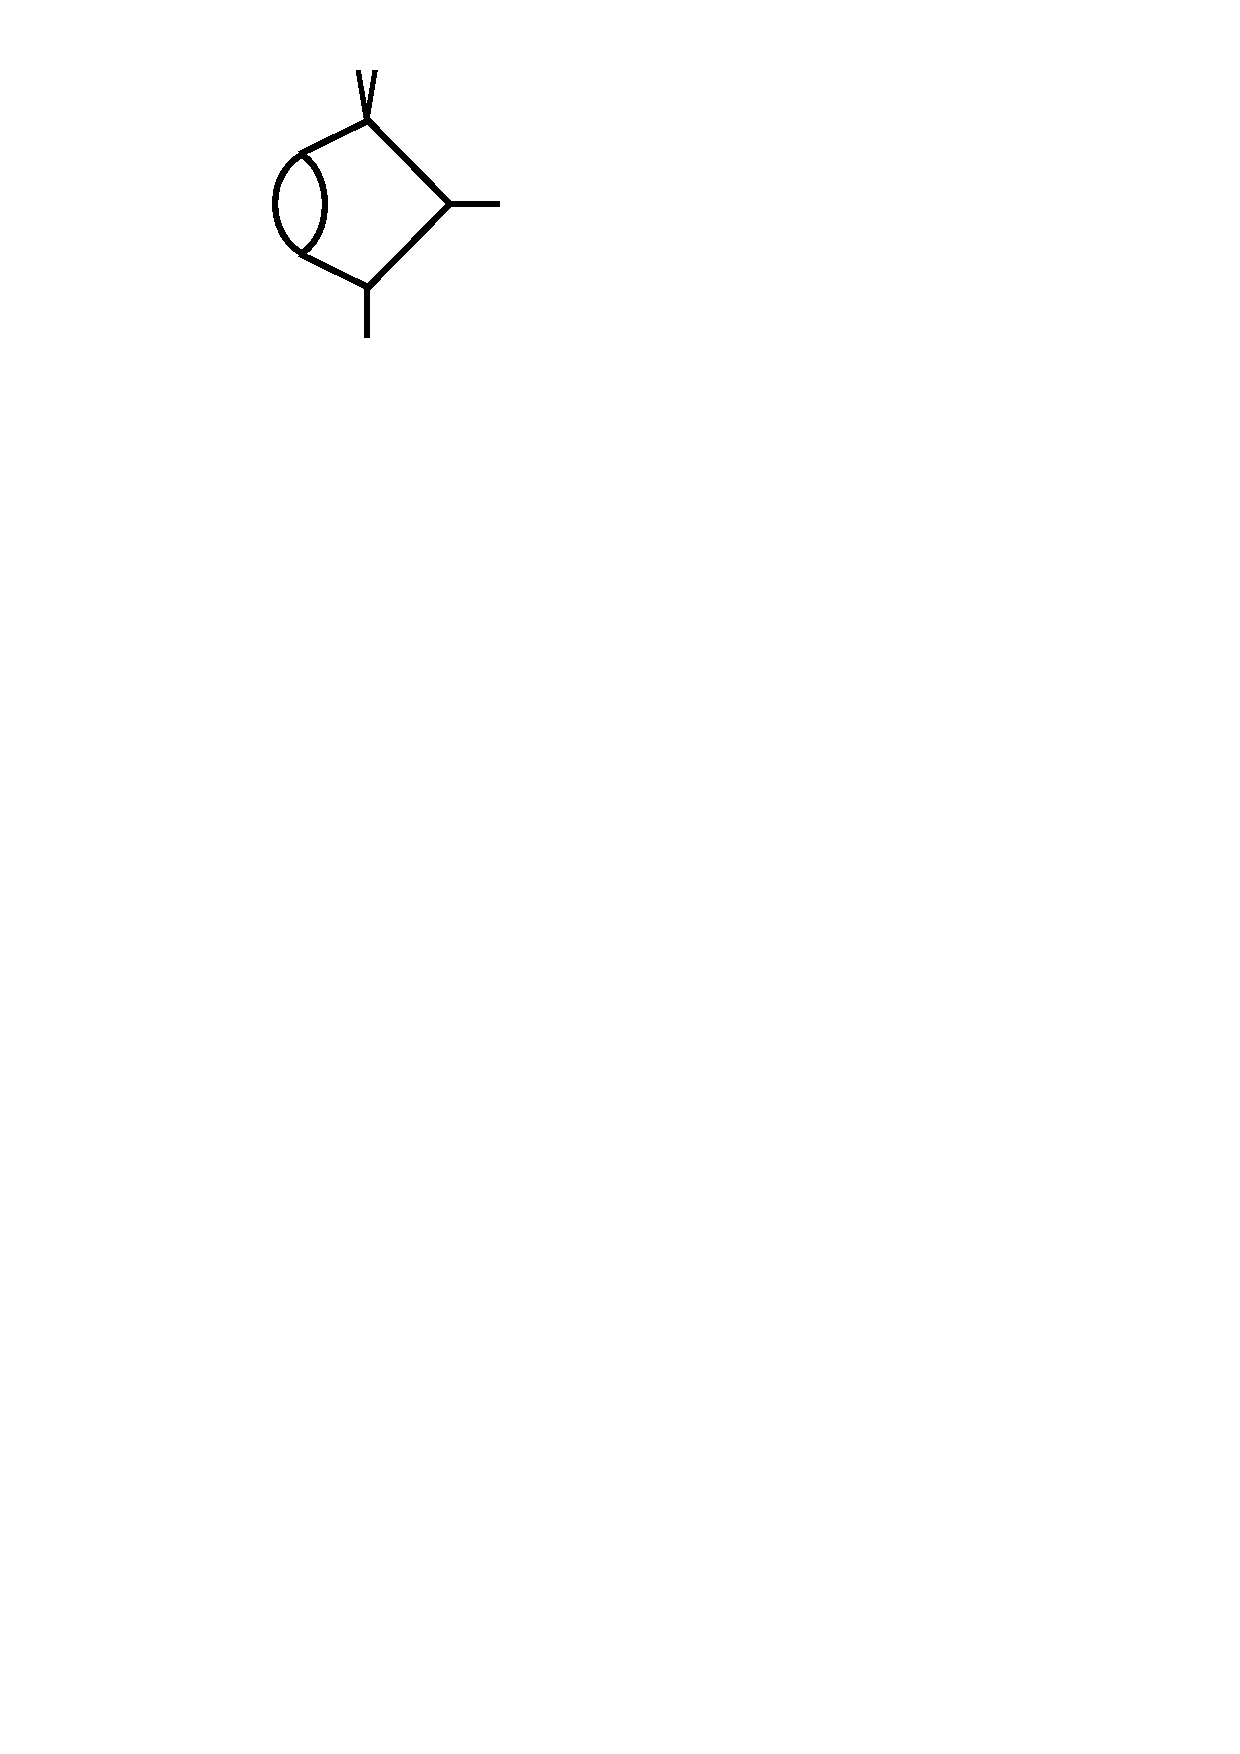
\includegraphics[scale=0.35]{figures/topologies/BubblePentagonRed1}};
      \node at
      (4,-5.5){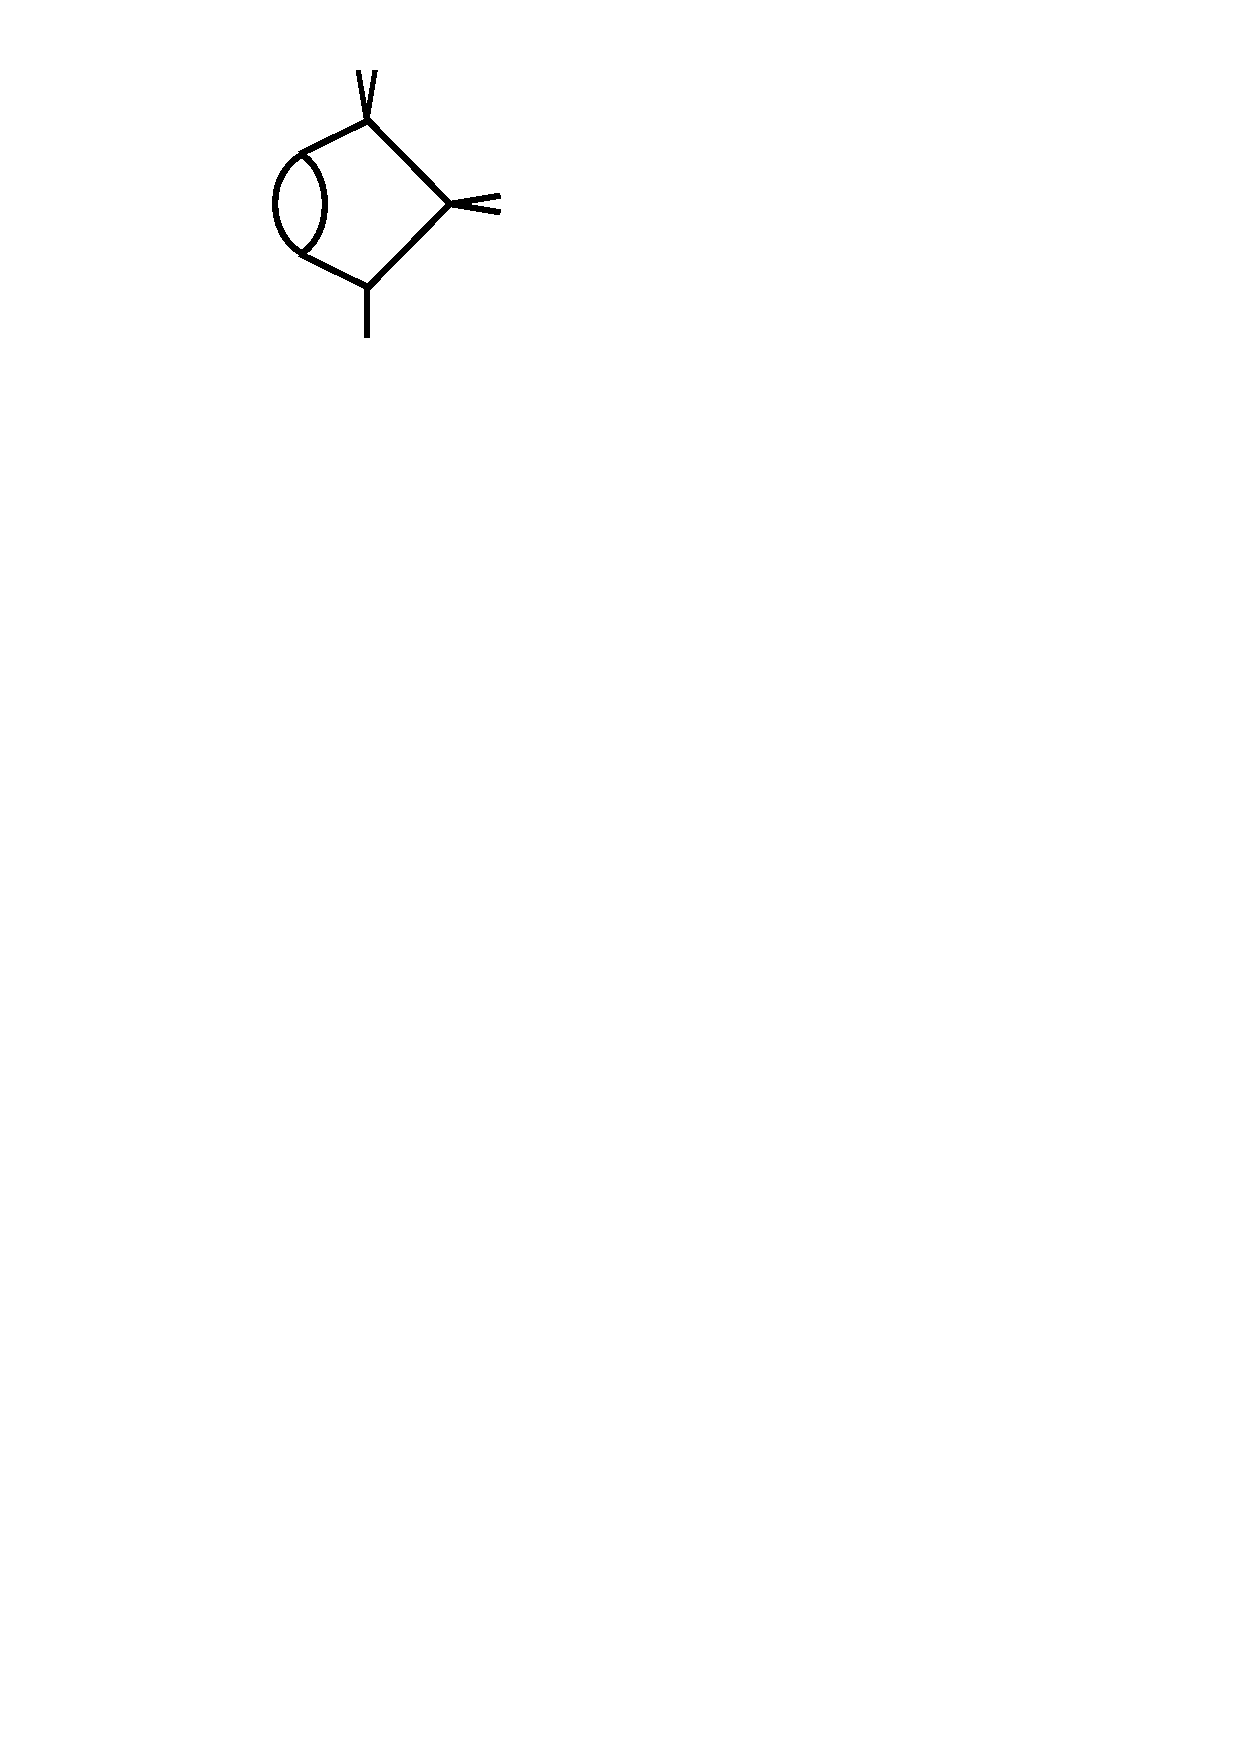
\includegraphics[scale=0.35]{figures/topologies/BubblePentagonRed2}};
      \node at
      (6,-5.5){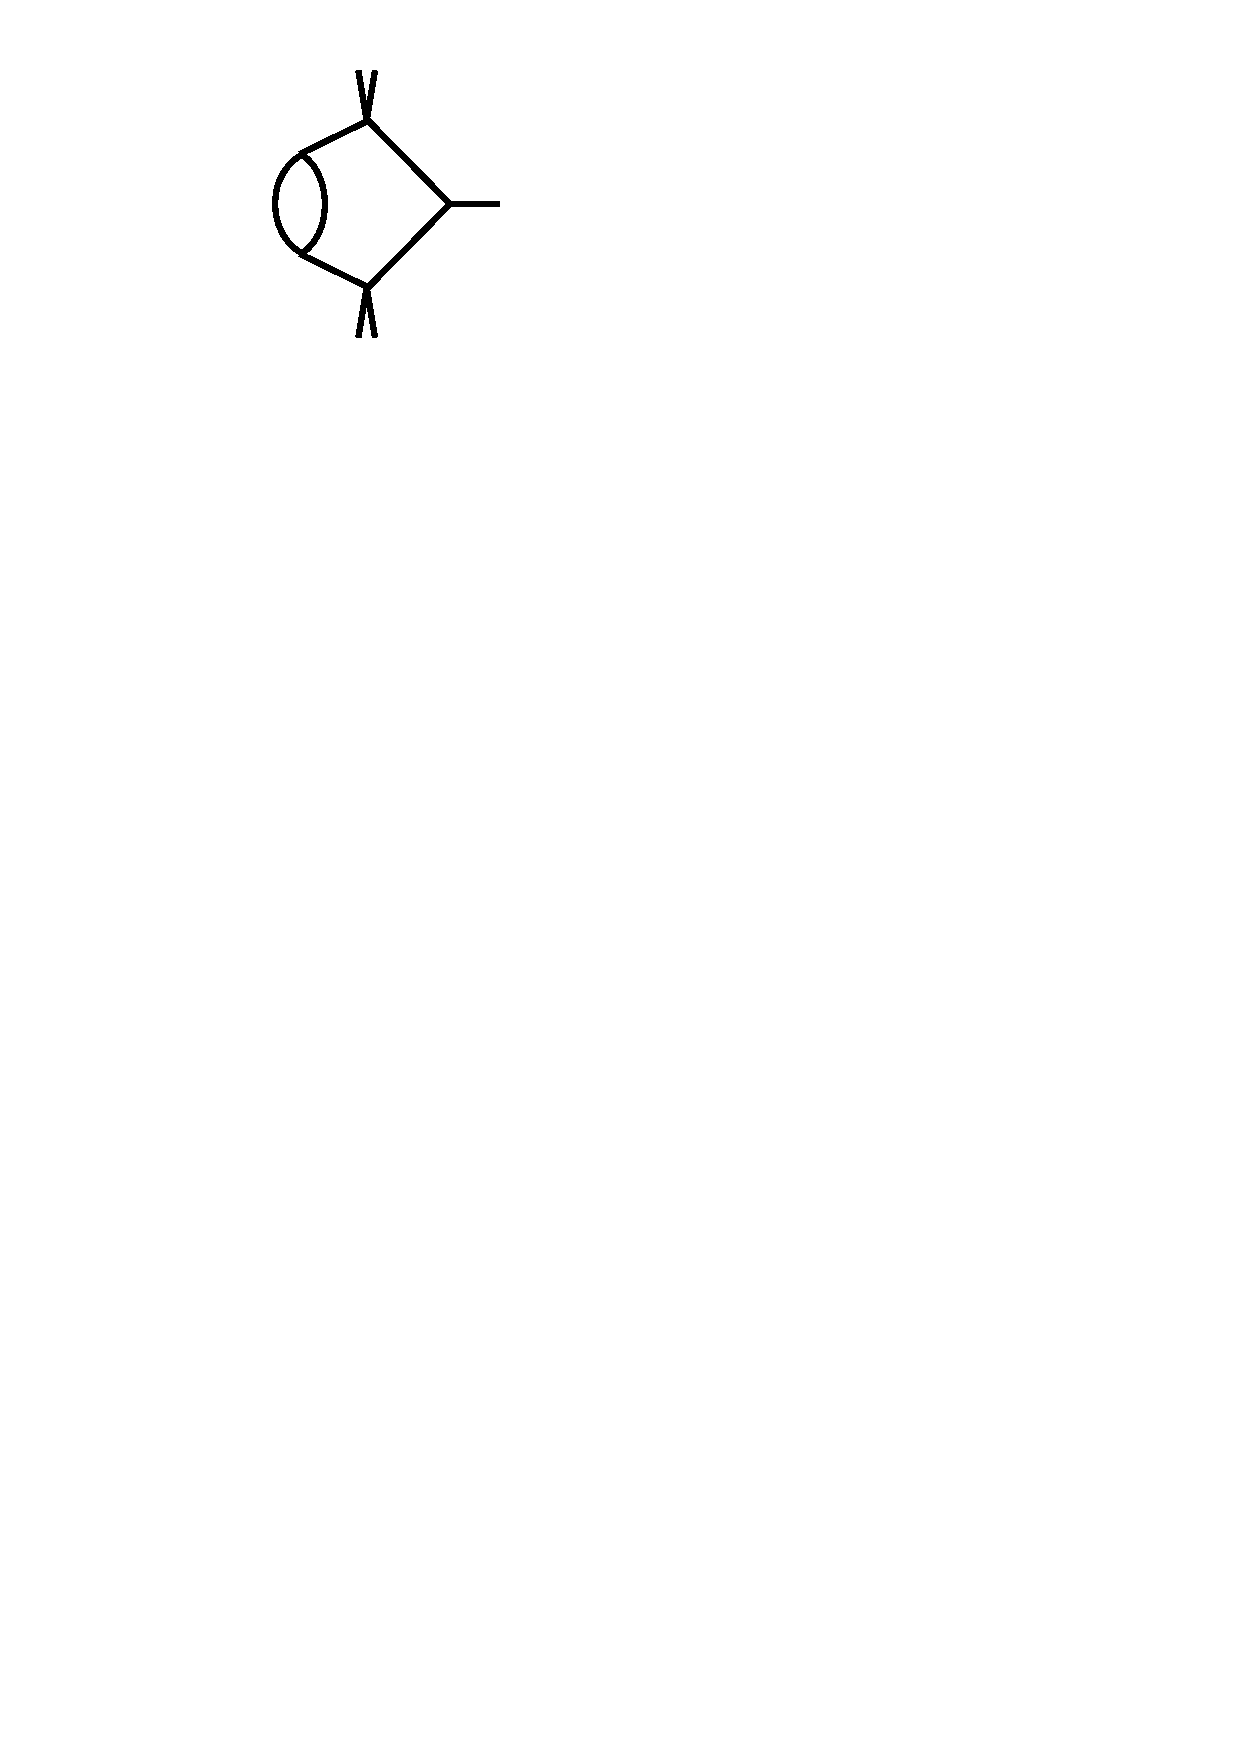
\includegraphics[scale=0.35]{figures/topologies/BubblePentagonRed3}};
      \node at
      (8,-5.5){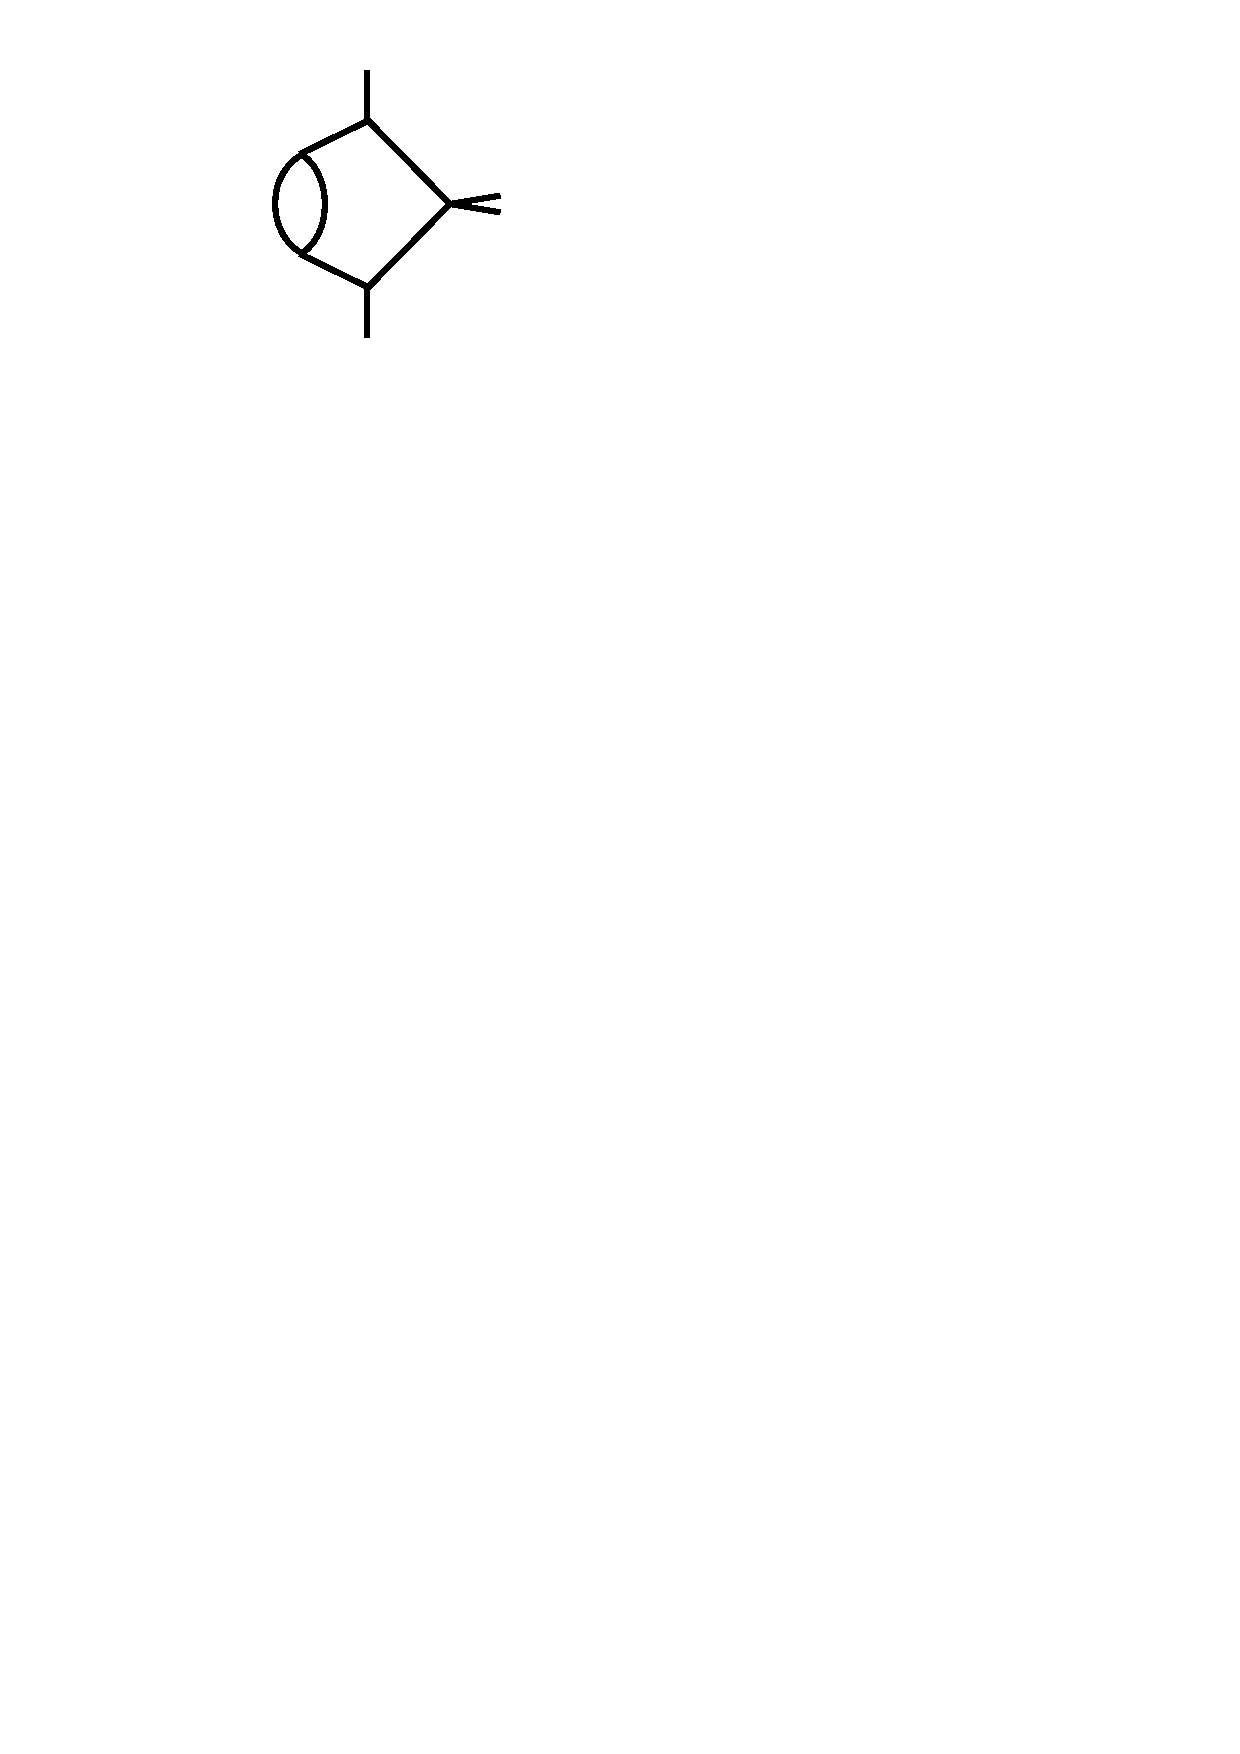
\includegraphics[scale=0.35]{figures/topologies/BubblePentagonRed4}};
      \node at
      (10,-5.5){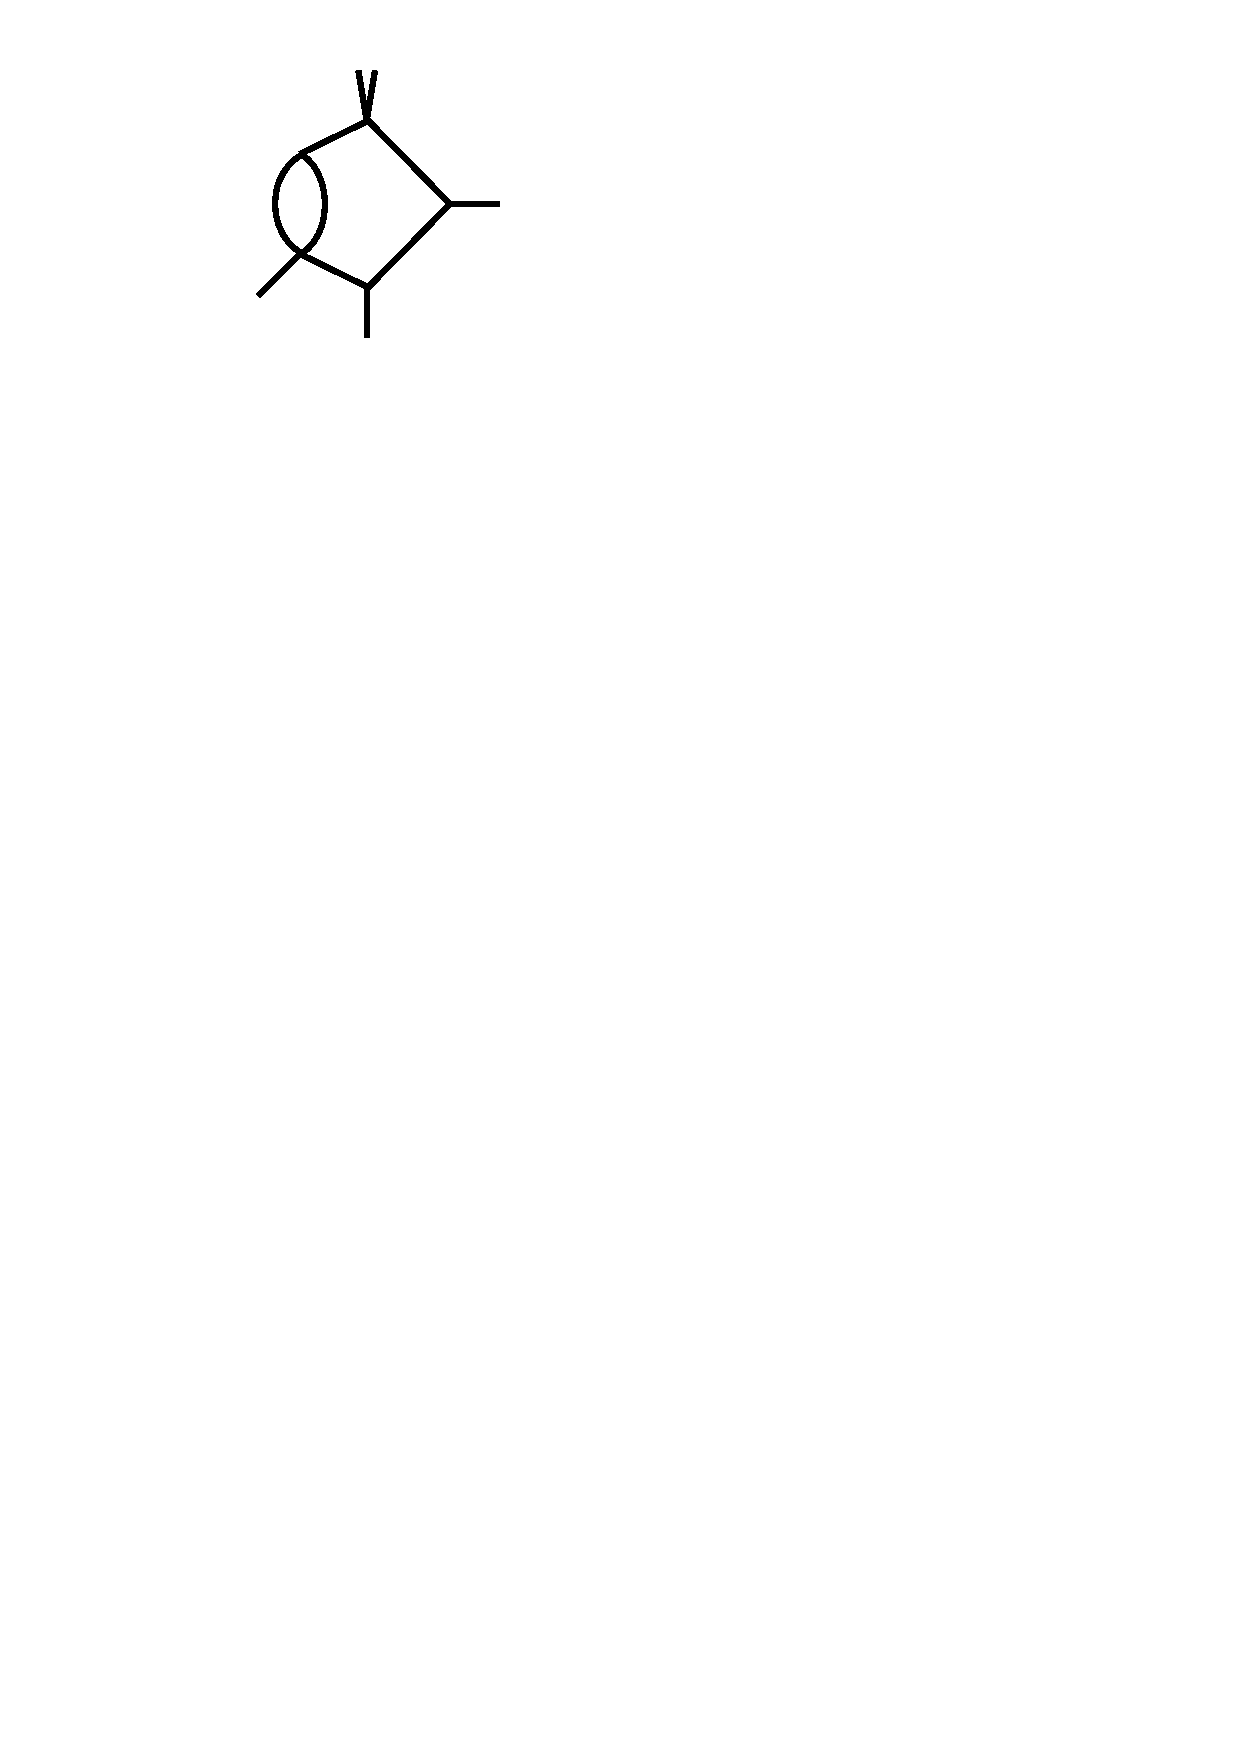
\includegraphics[scale=0.35]{figures/topologies/BubblePentagonRed5}};
    %
      \node at
      (0,-7){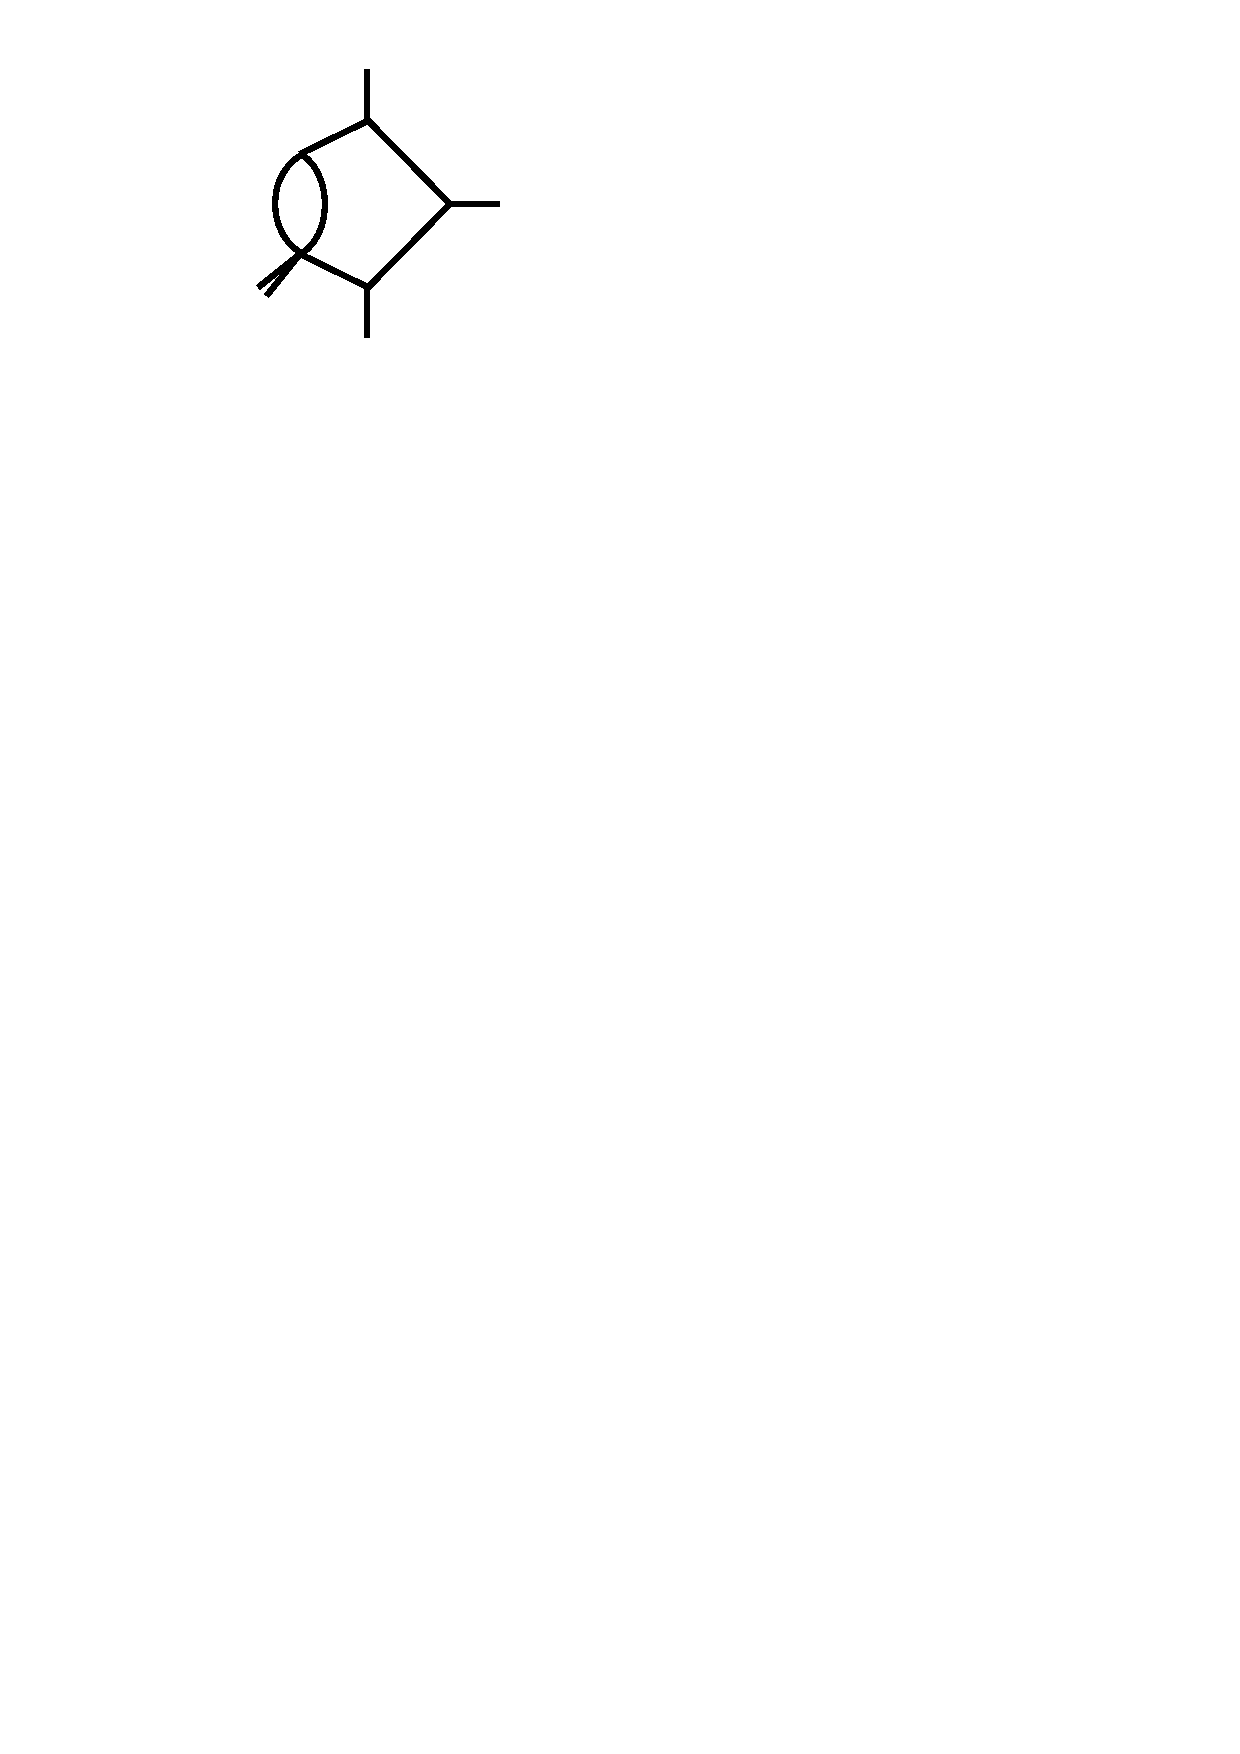
\includegraphics[scale=0.35]{figures/topologies/BubblePentagonRed6}};
      \node at
      (2,-7){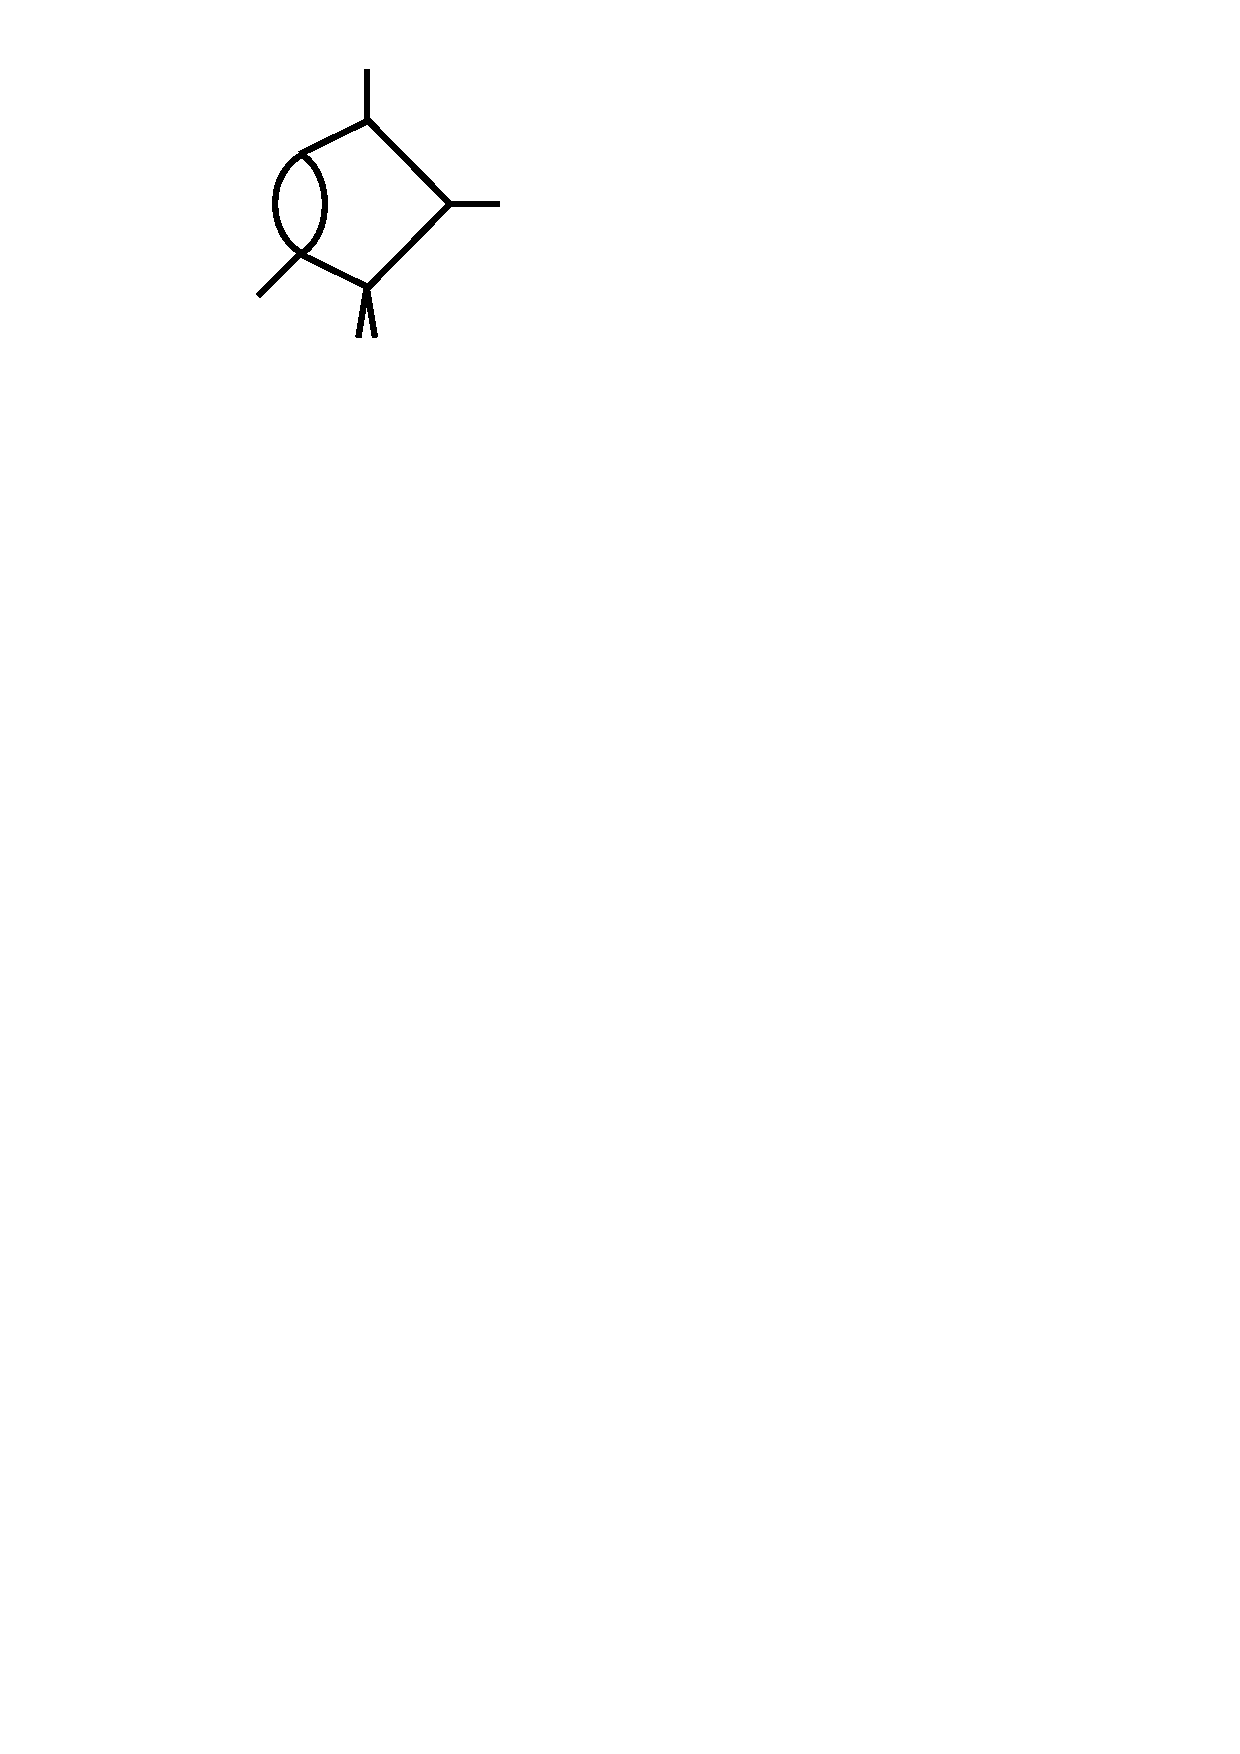
\includegraphics[scale=0.35]{figures/topologies/BubblePentagonRed7}};
      \node at
      (4,-7){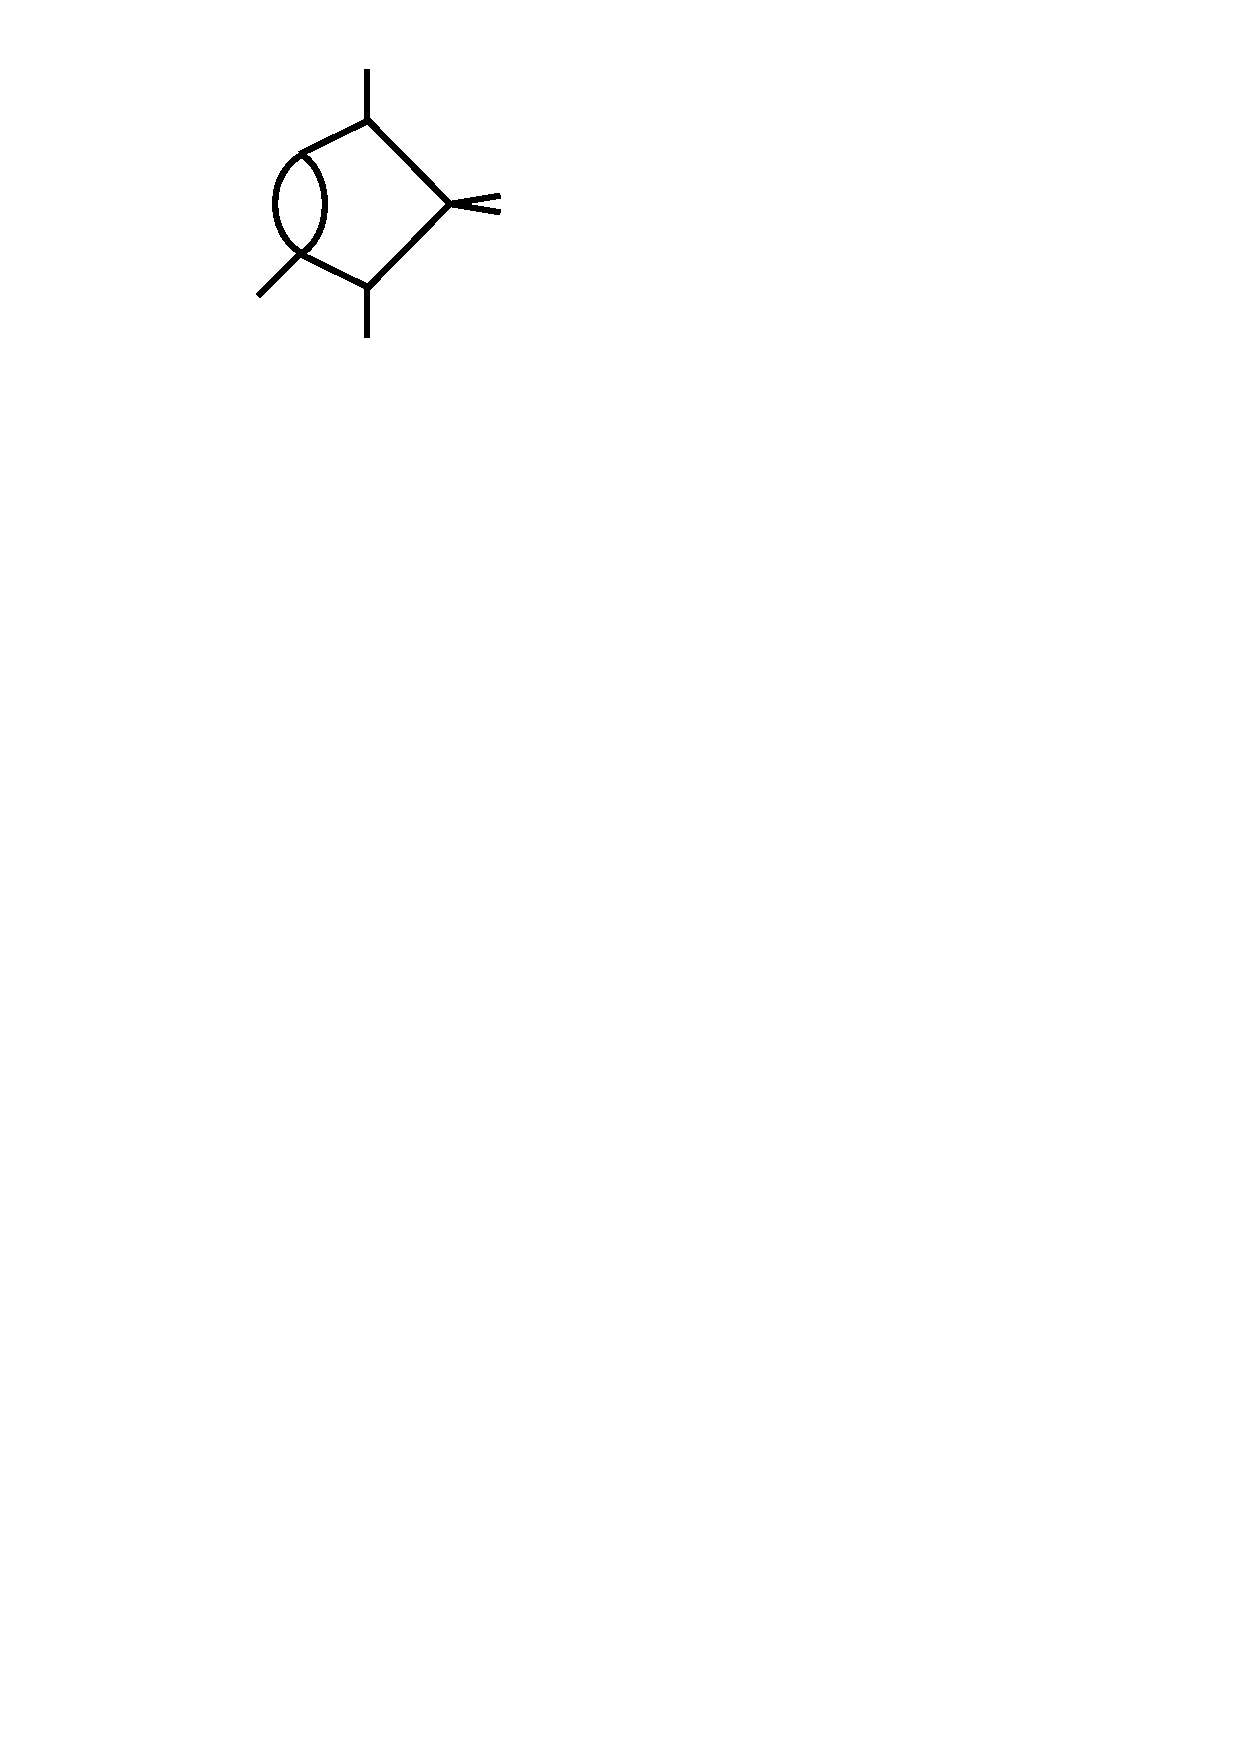
\includegraphics[scale=0.35]{figures/topologies/BubblePentagonRed8}};
      \node at
      (6,-7){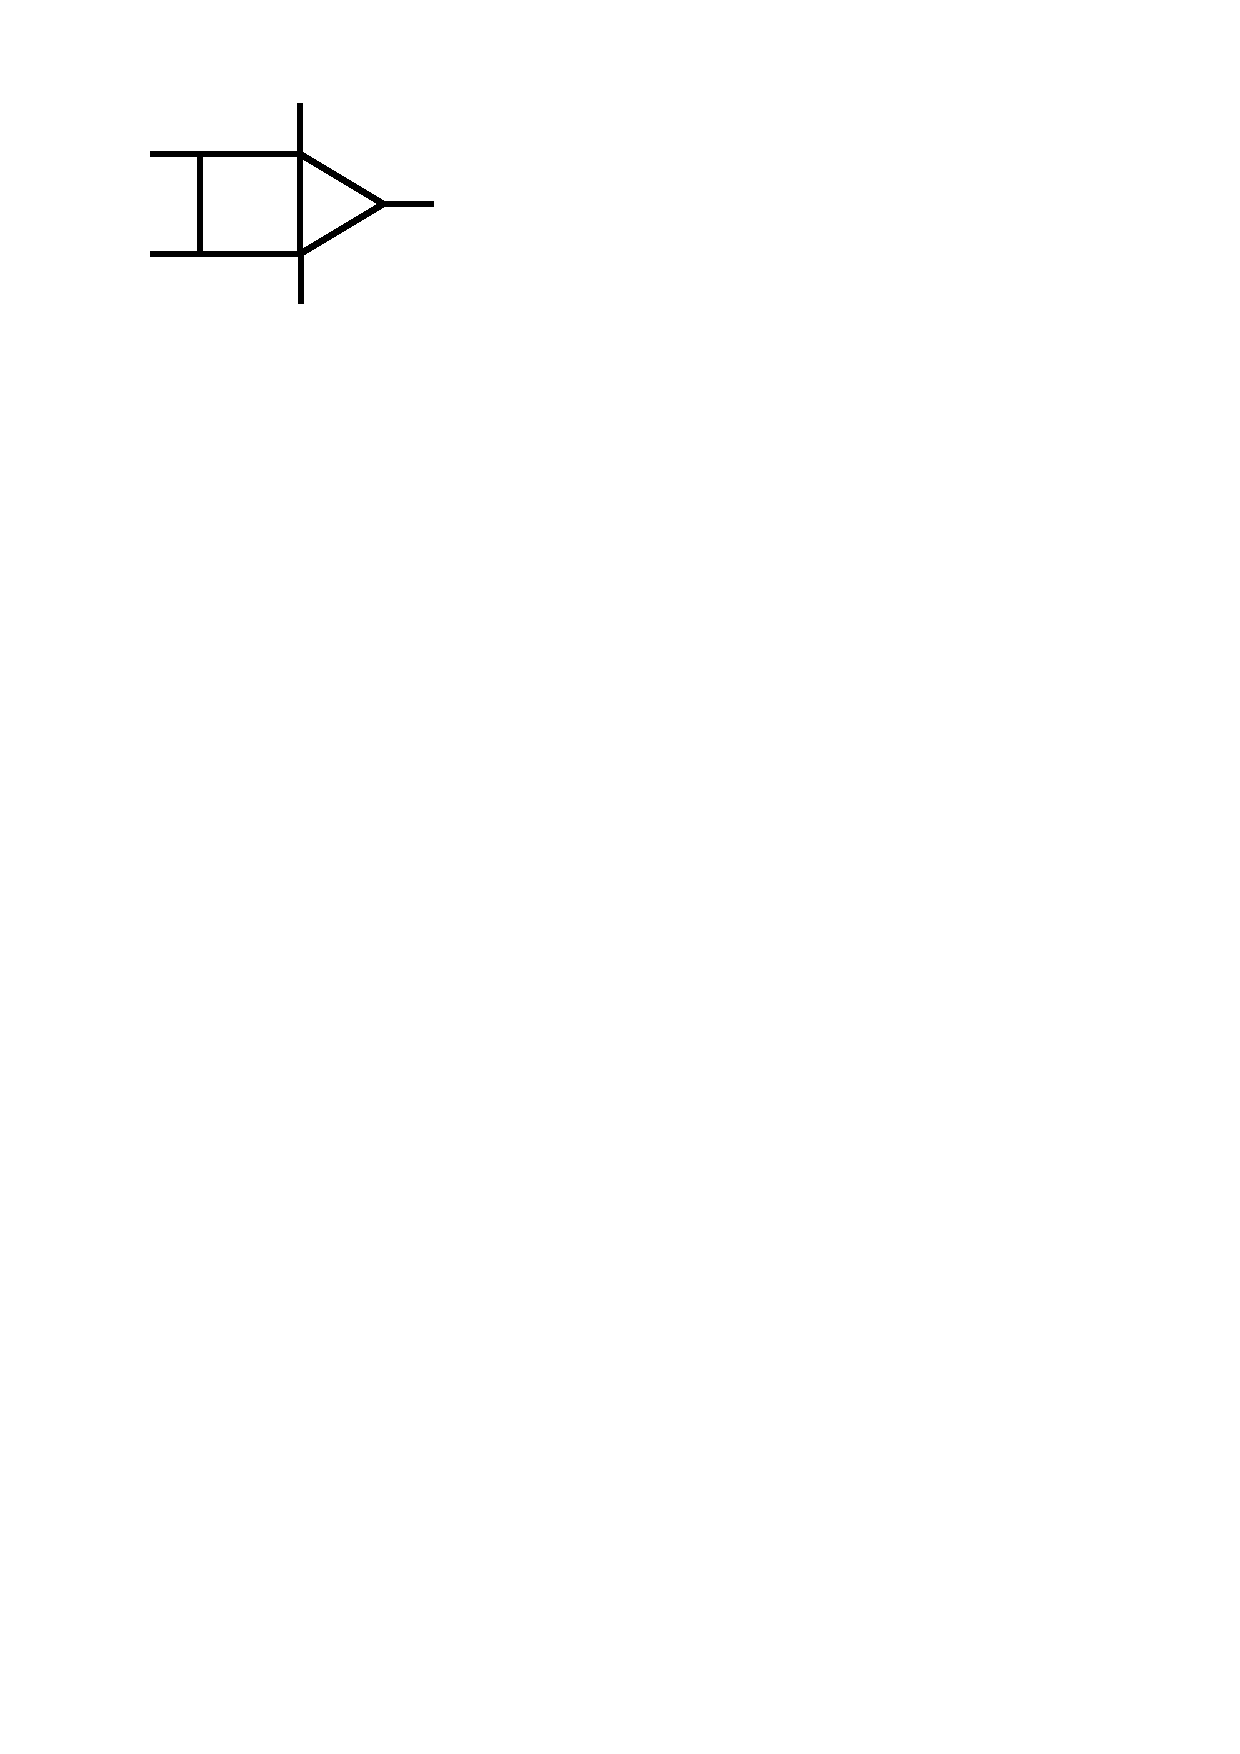
\includegraphics[scale=0.4]{figures/topologies/BoxTriangleG}};
      \node at
      (8,-6.9){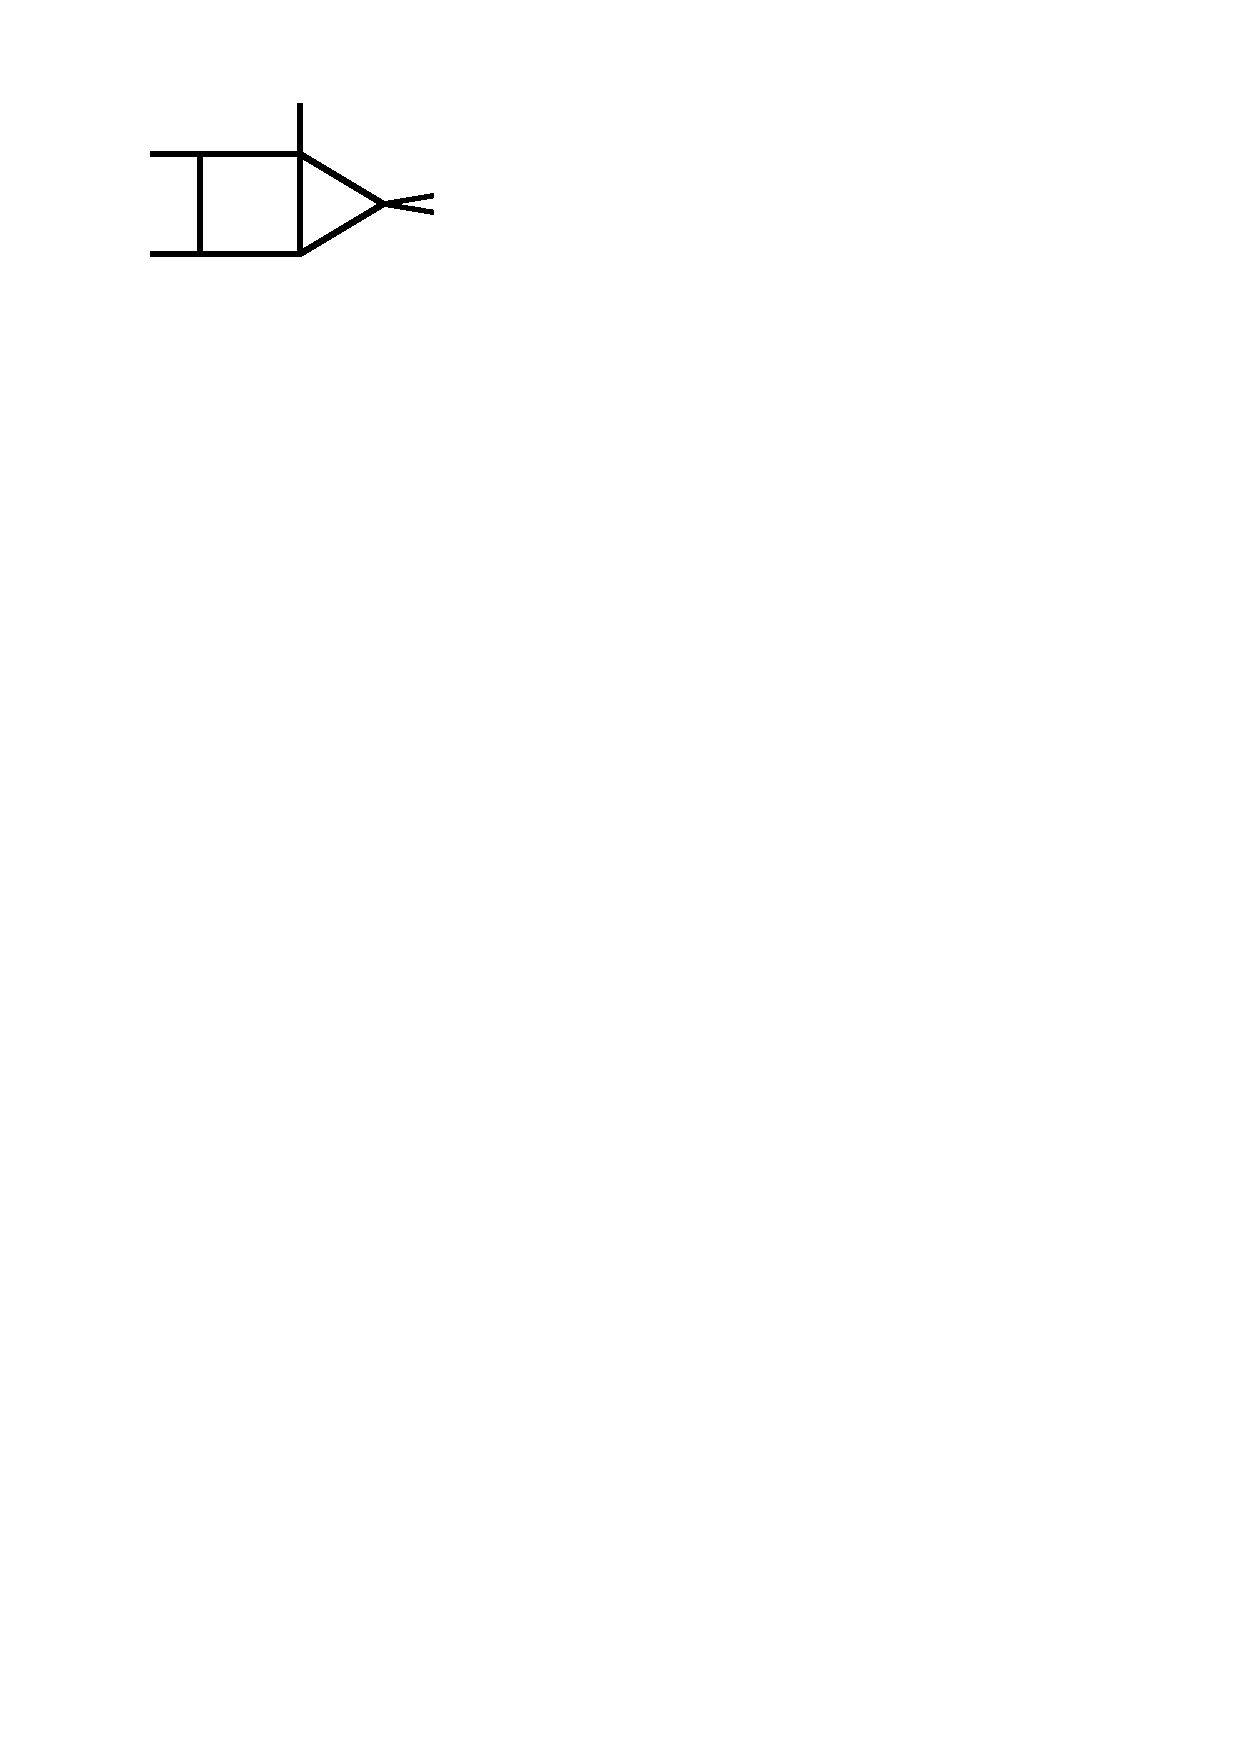
\includegraphics[scale=0.4]{figures/topologies/BoxTriangleSG}};
      \node at
      (10,-6.9){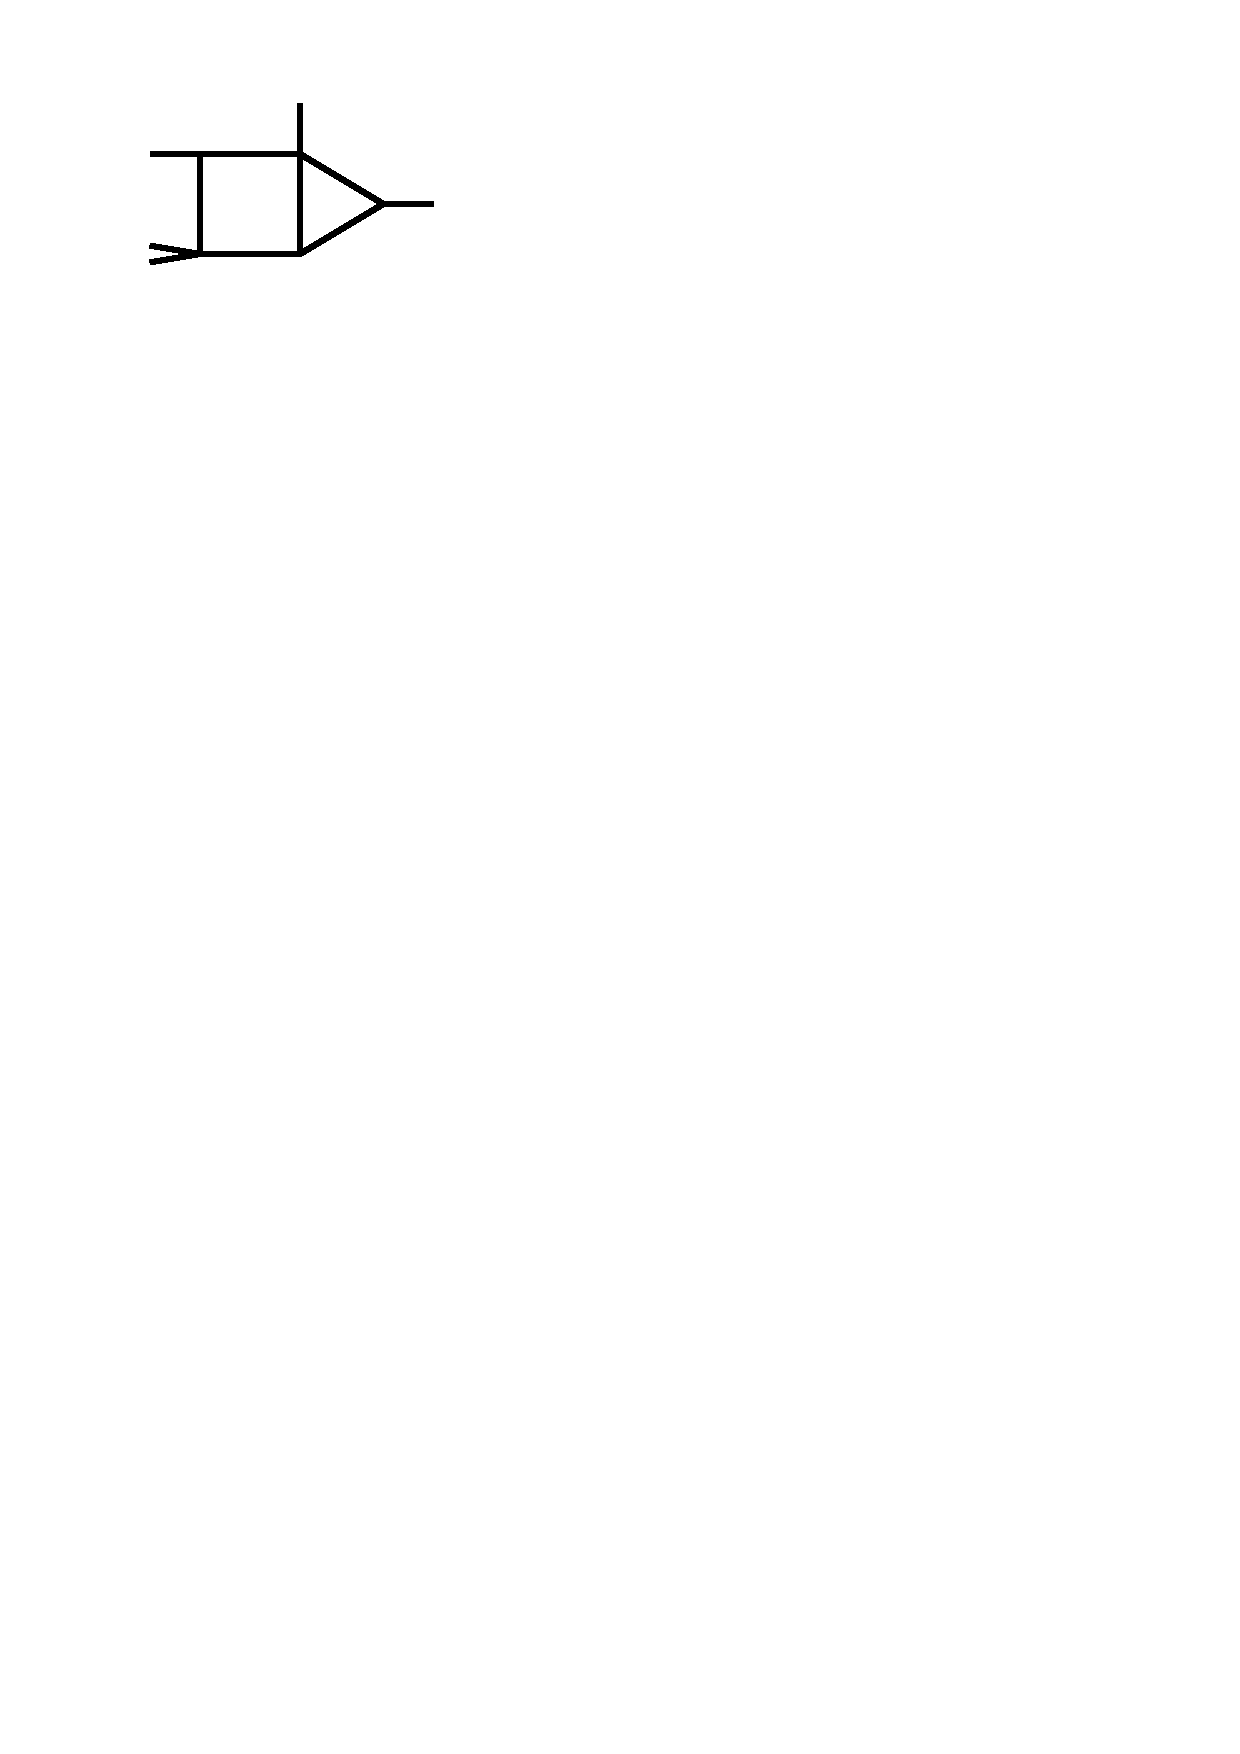
\includegraphics[scale=0.4]{figures/topologies/BoxTriangleRed1}};
    %
      \node at
      (0,-8.4){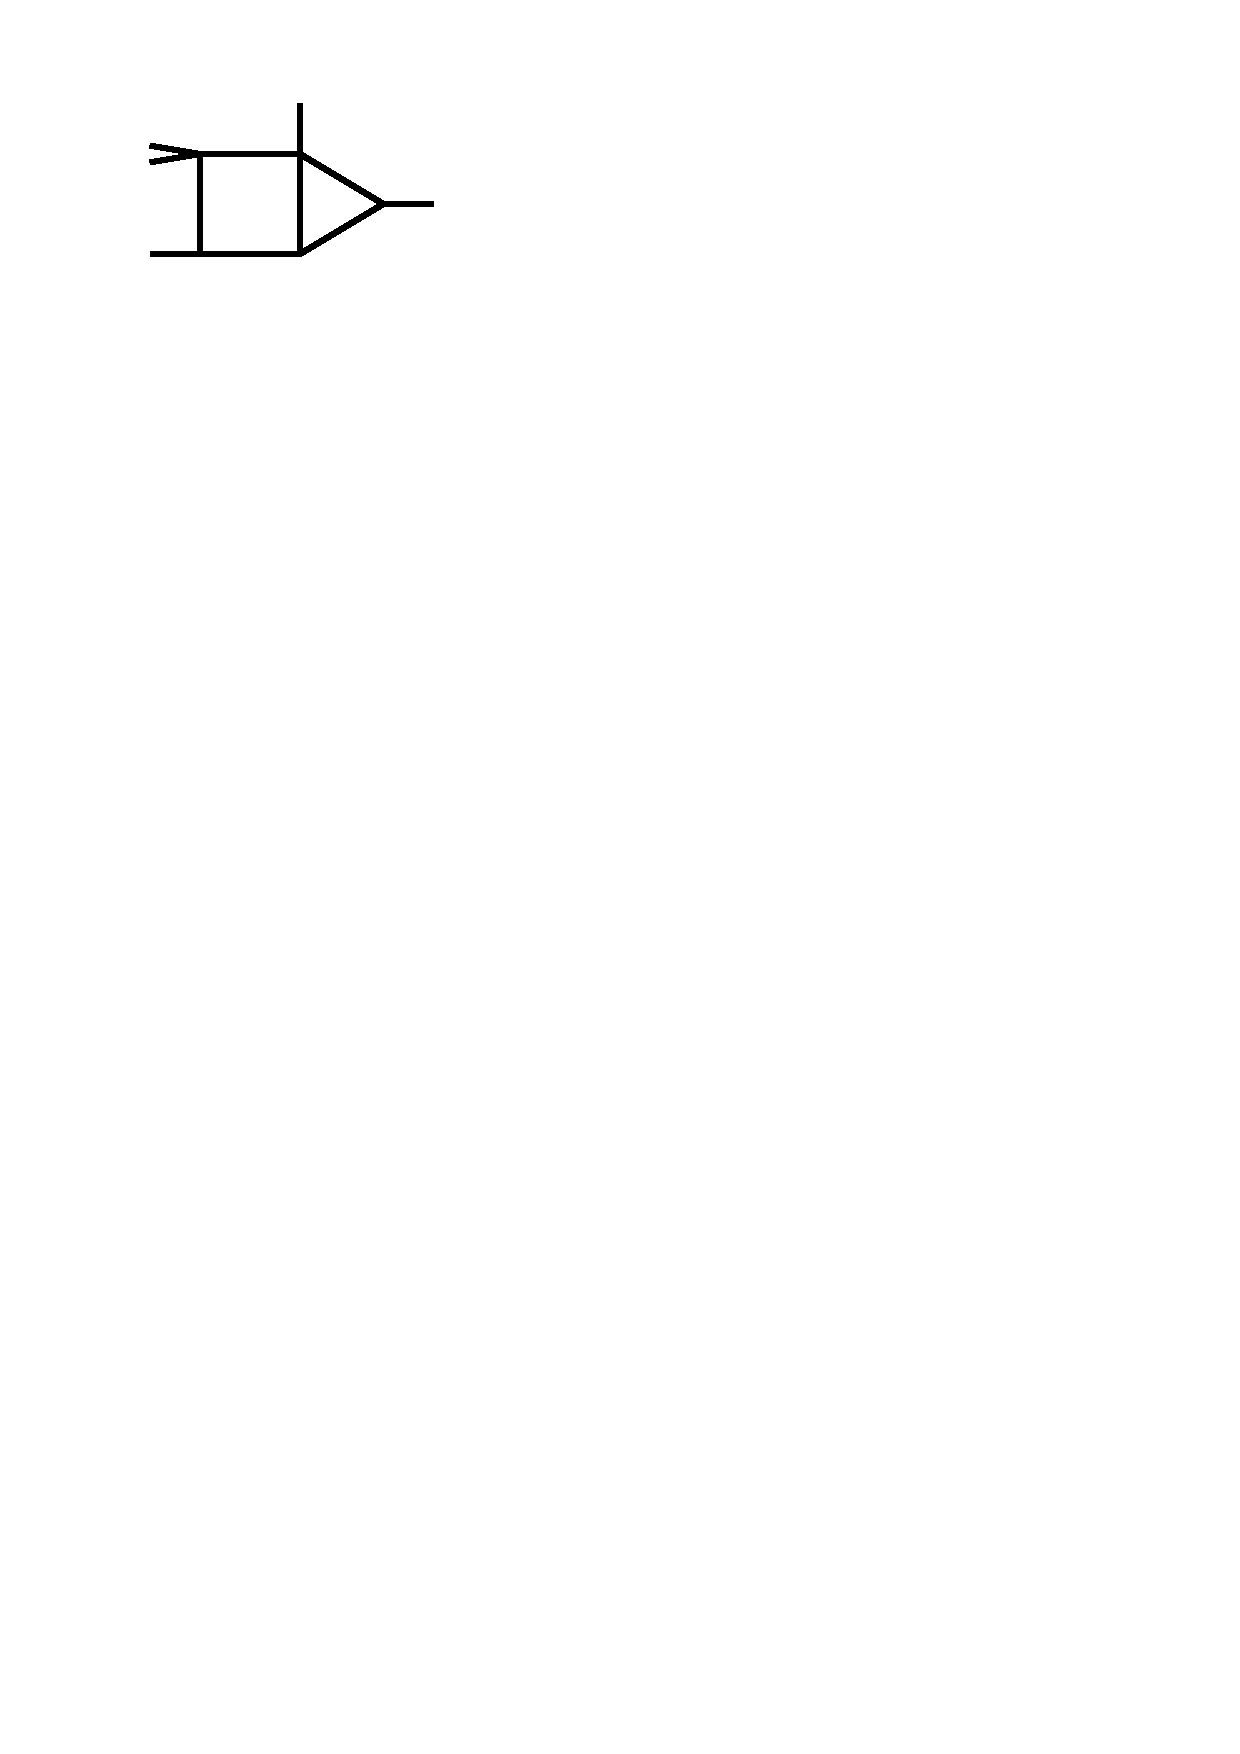
\includegraphics[scale=0.4]{figures/topologies/BoxTriangleRed2}};
      \node at
      (2,-8.4){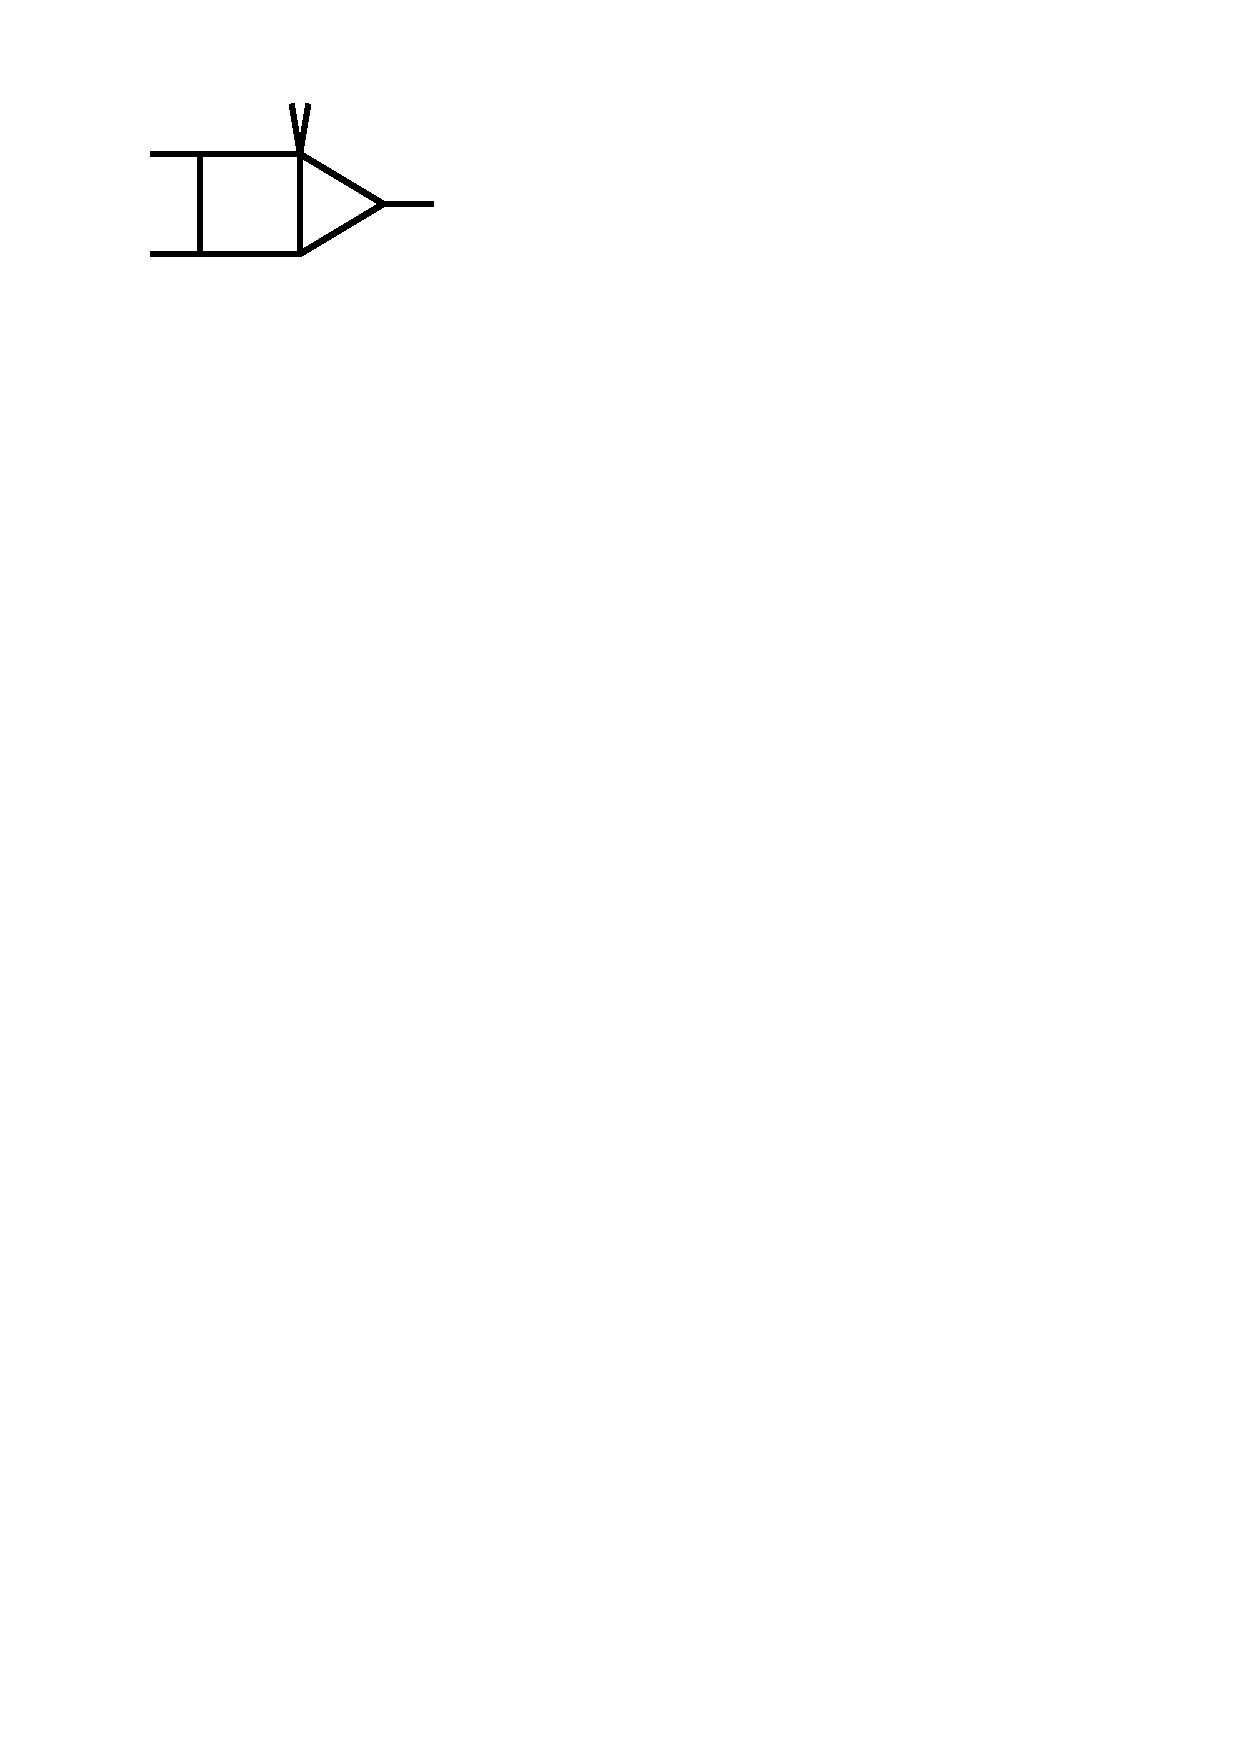
\includegraphics[scale=0.4]{figures/topologies/BoxTriangleRed3}};
      \node at
      (4,-8.5){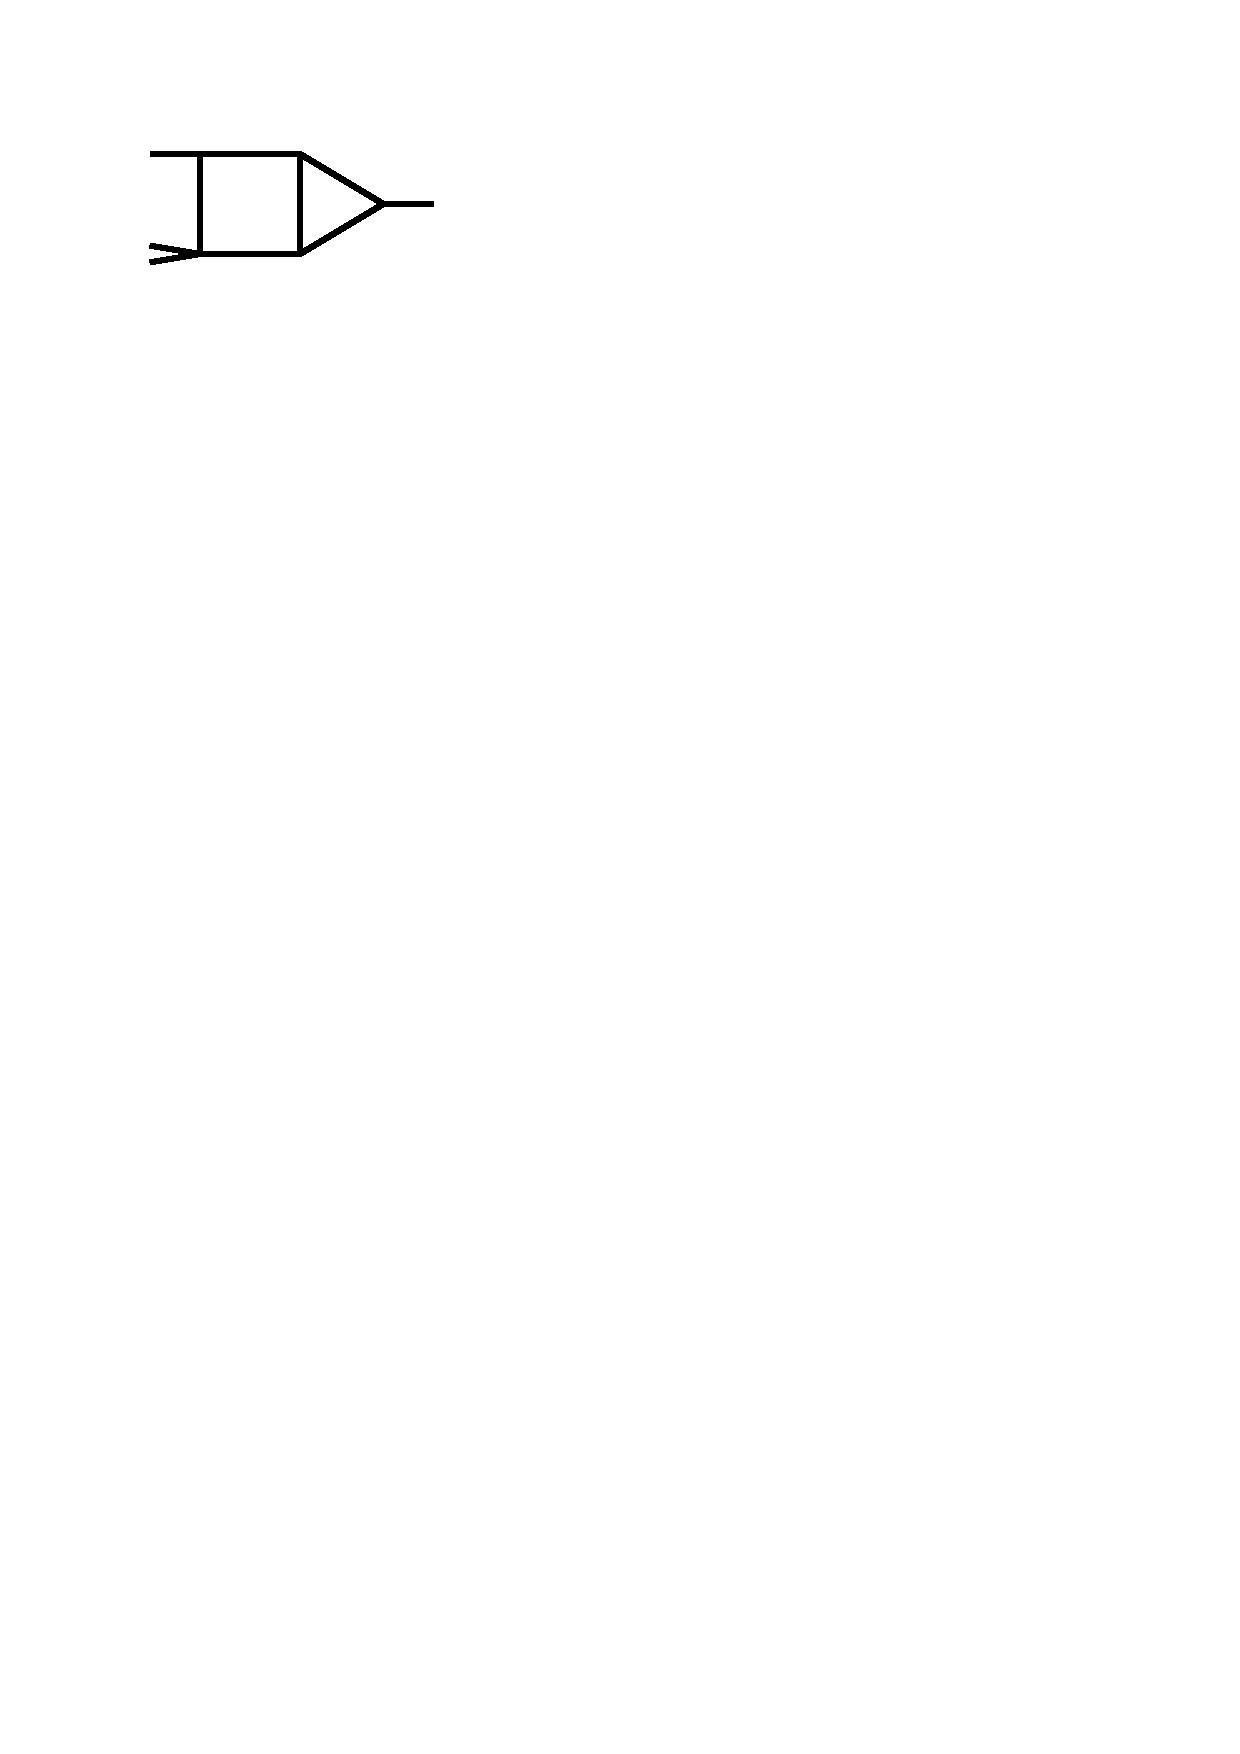
\includegraphics[scale=0.4]{figures/topologies/BoxTriangleRed4}};
      \node at
      (6,-8.5){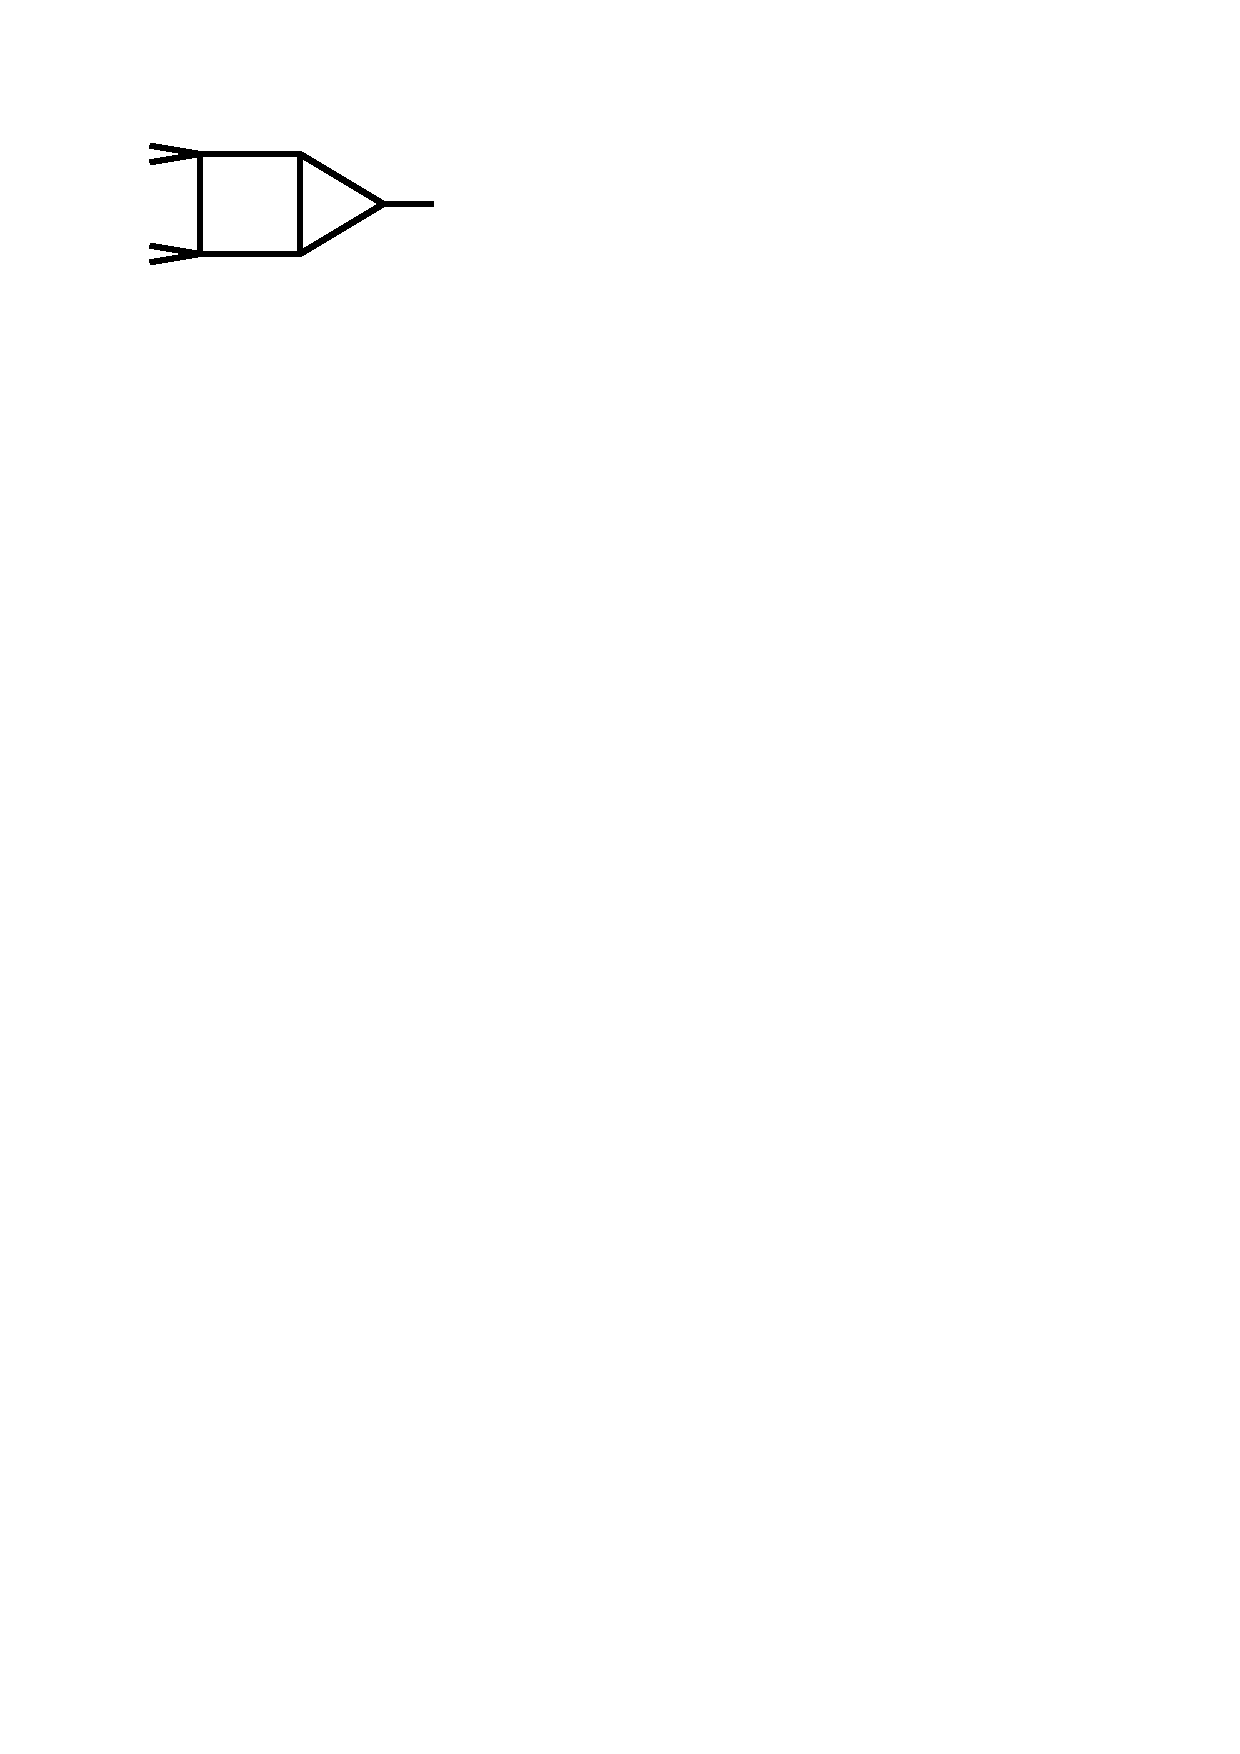
\includegraphics[scale=0.4]{figures/topologies/BoxTriangleRed5}};
      \node at
      (8,-8.5){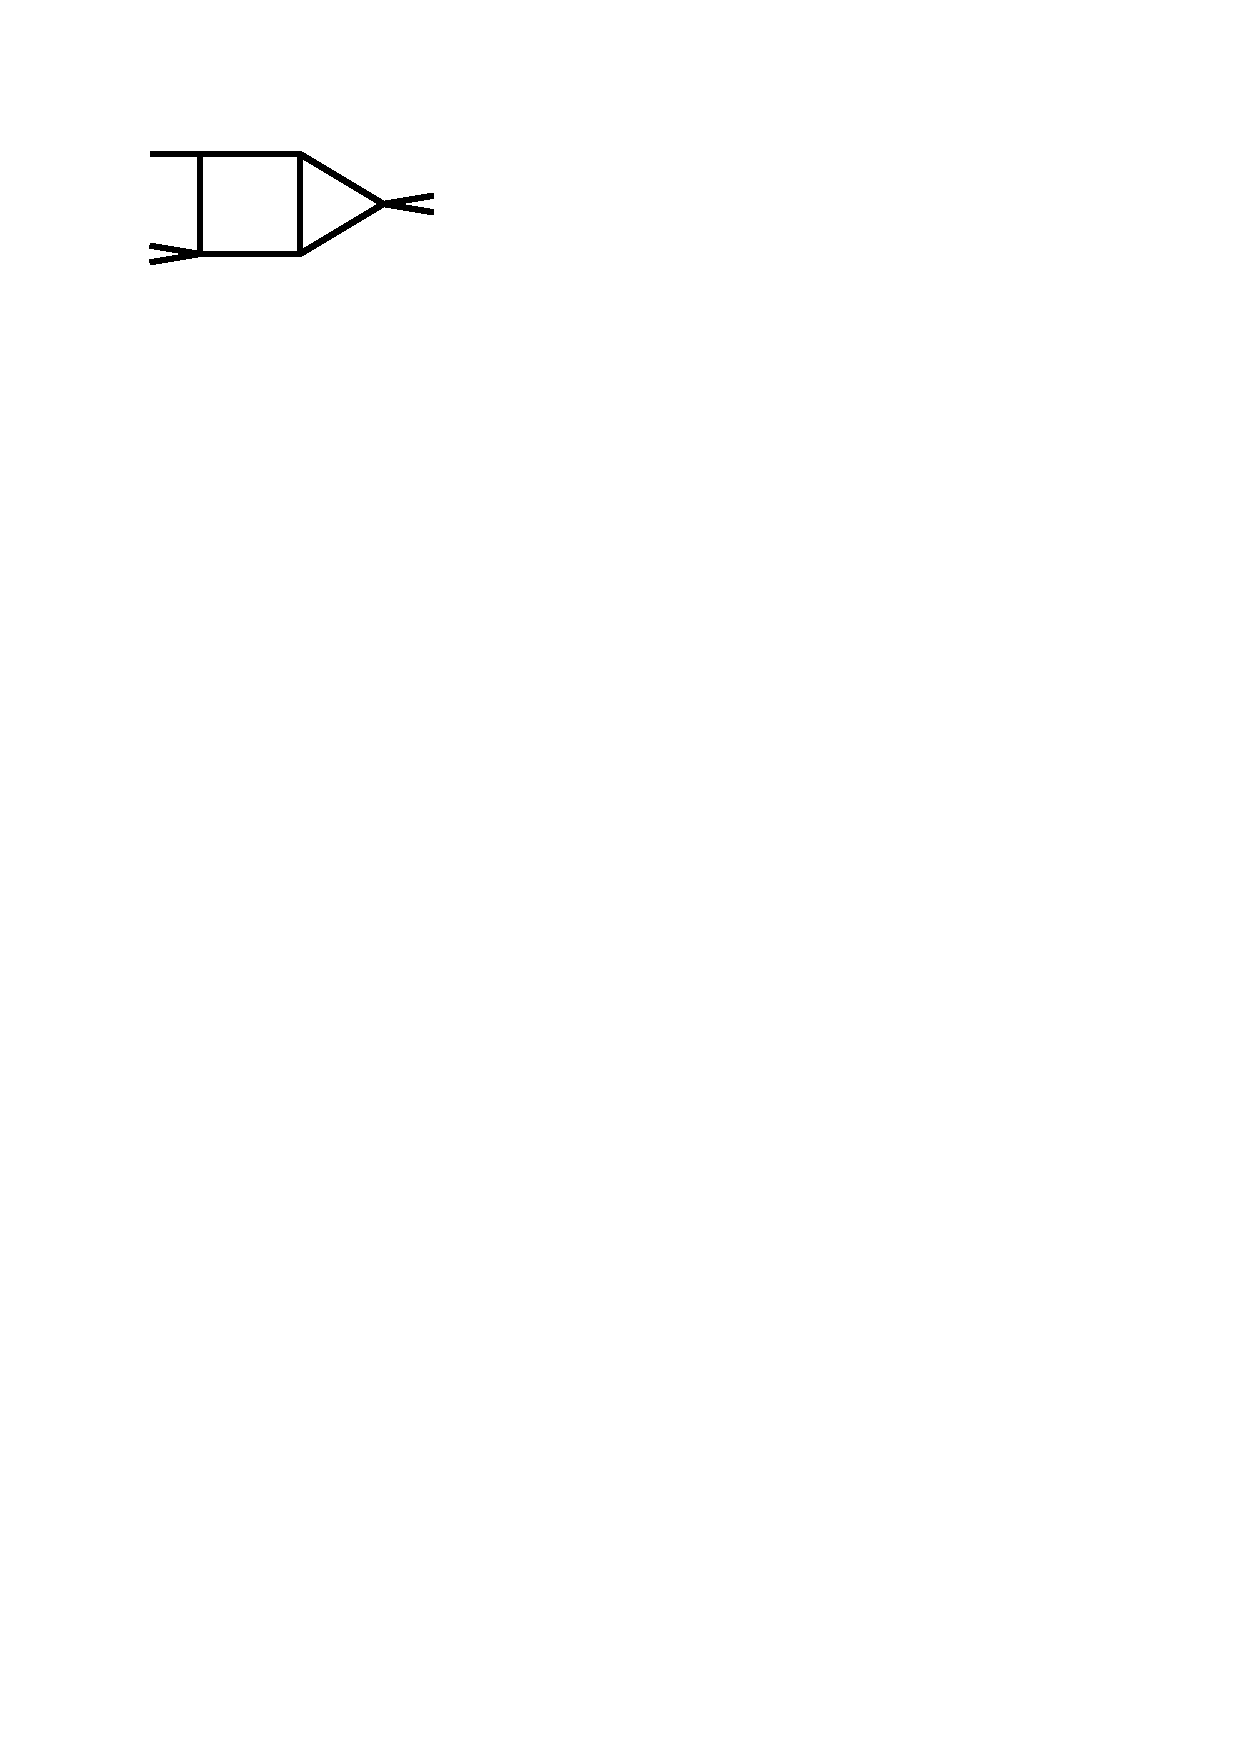
\includegraphics[scale=0.4]{figures/topologies/BoxTriangleRed6}};
      \node at
      (10,-8.5){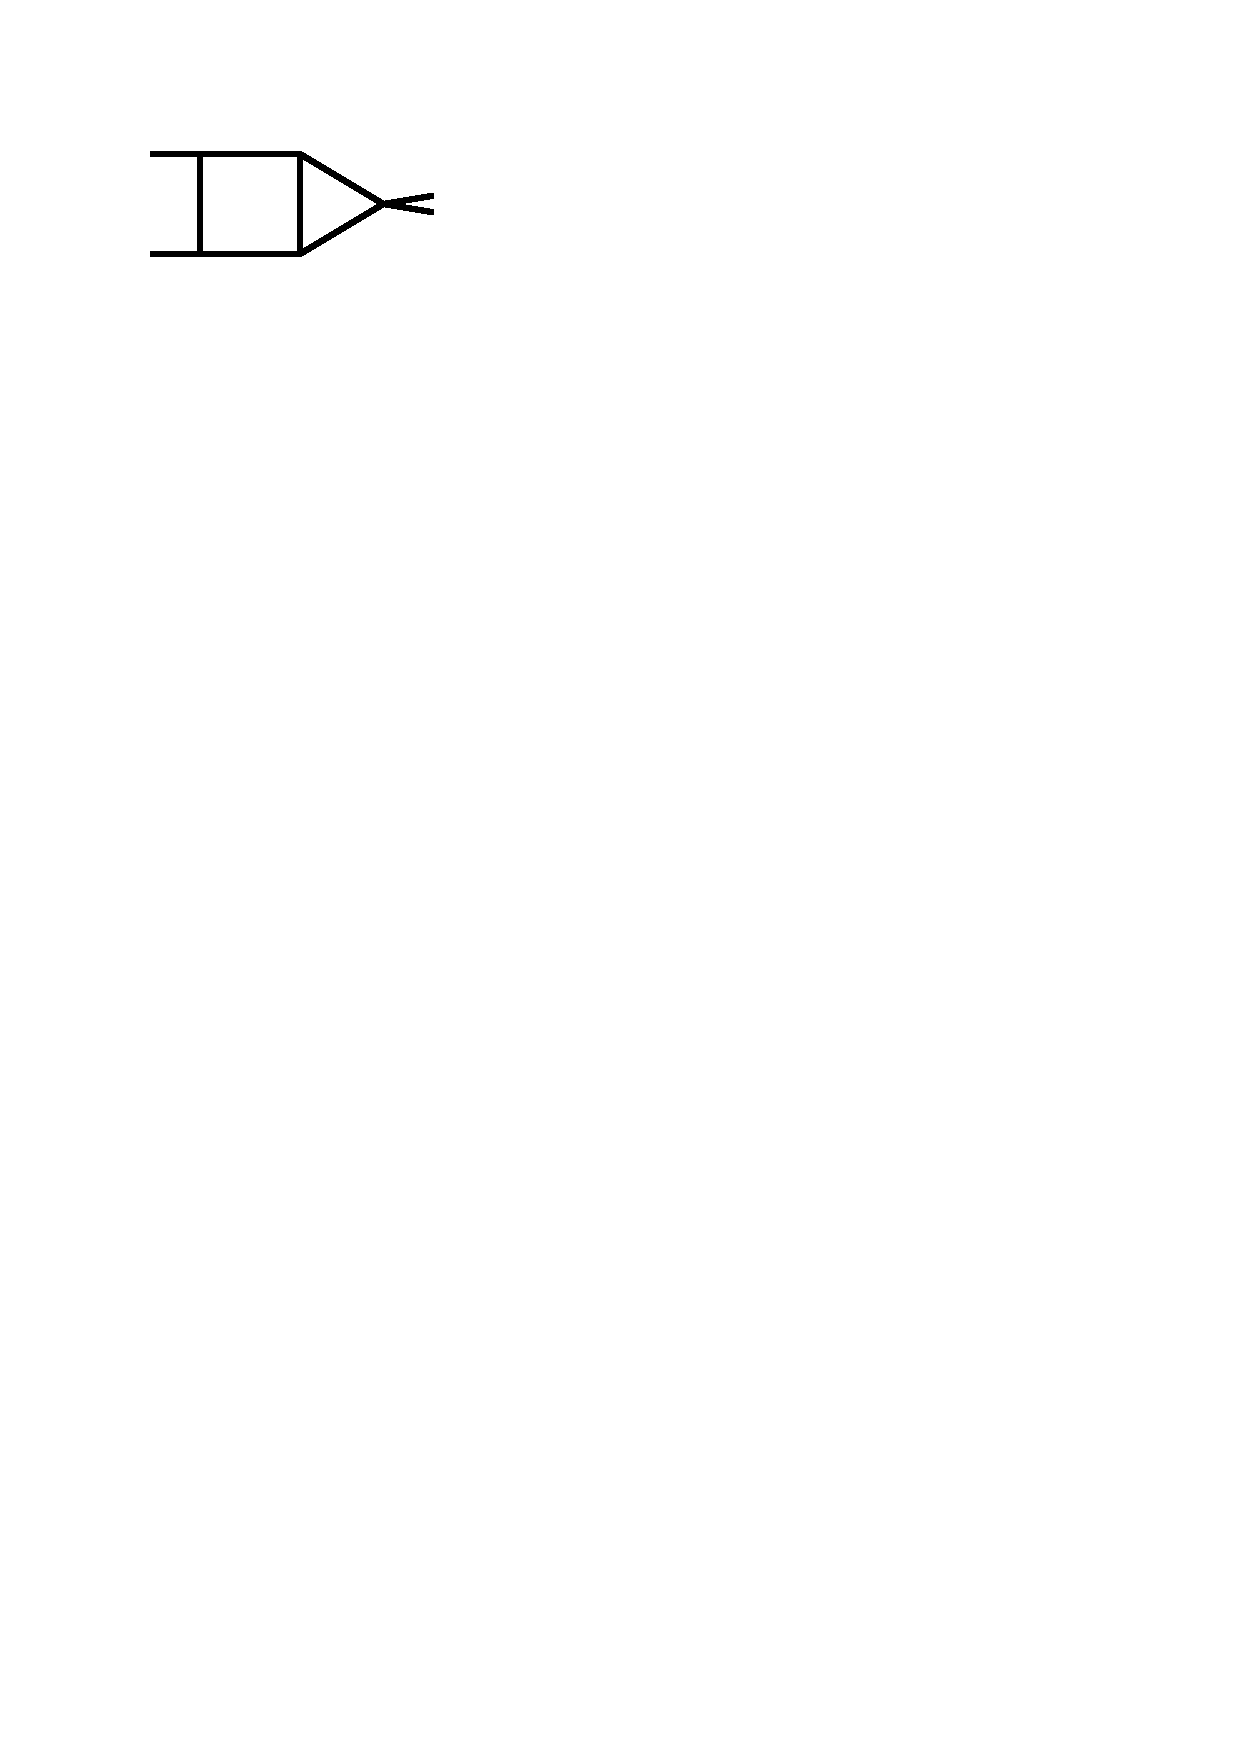
\includegraphics[scale=0.4]{figures/topologies/BoxTriangleRed7}};
    %
      \node at
      (3,-9.8){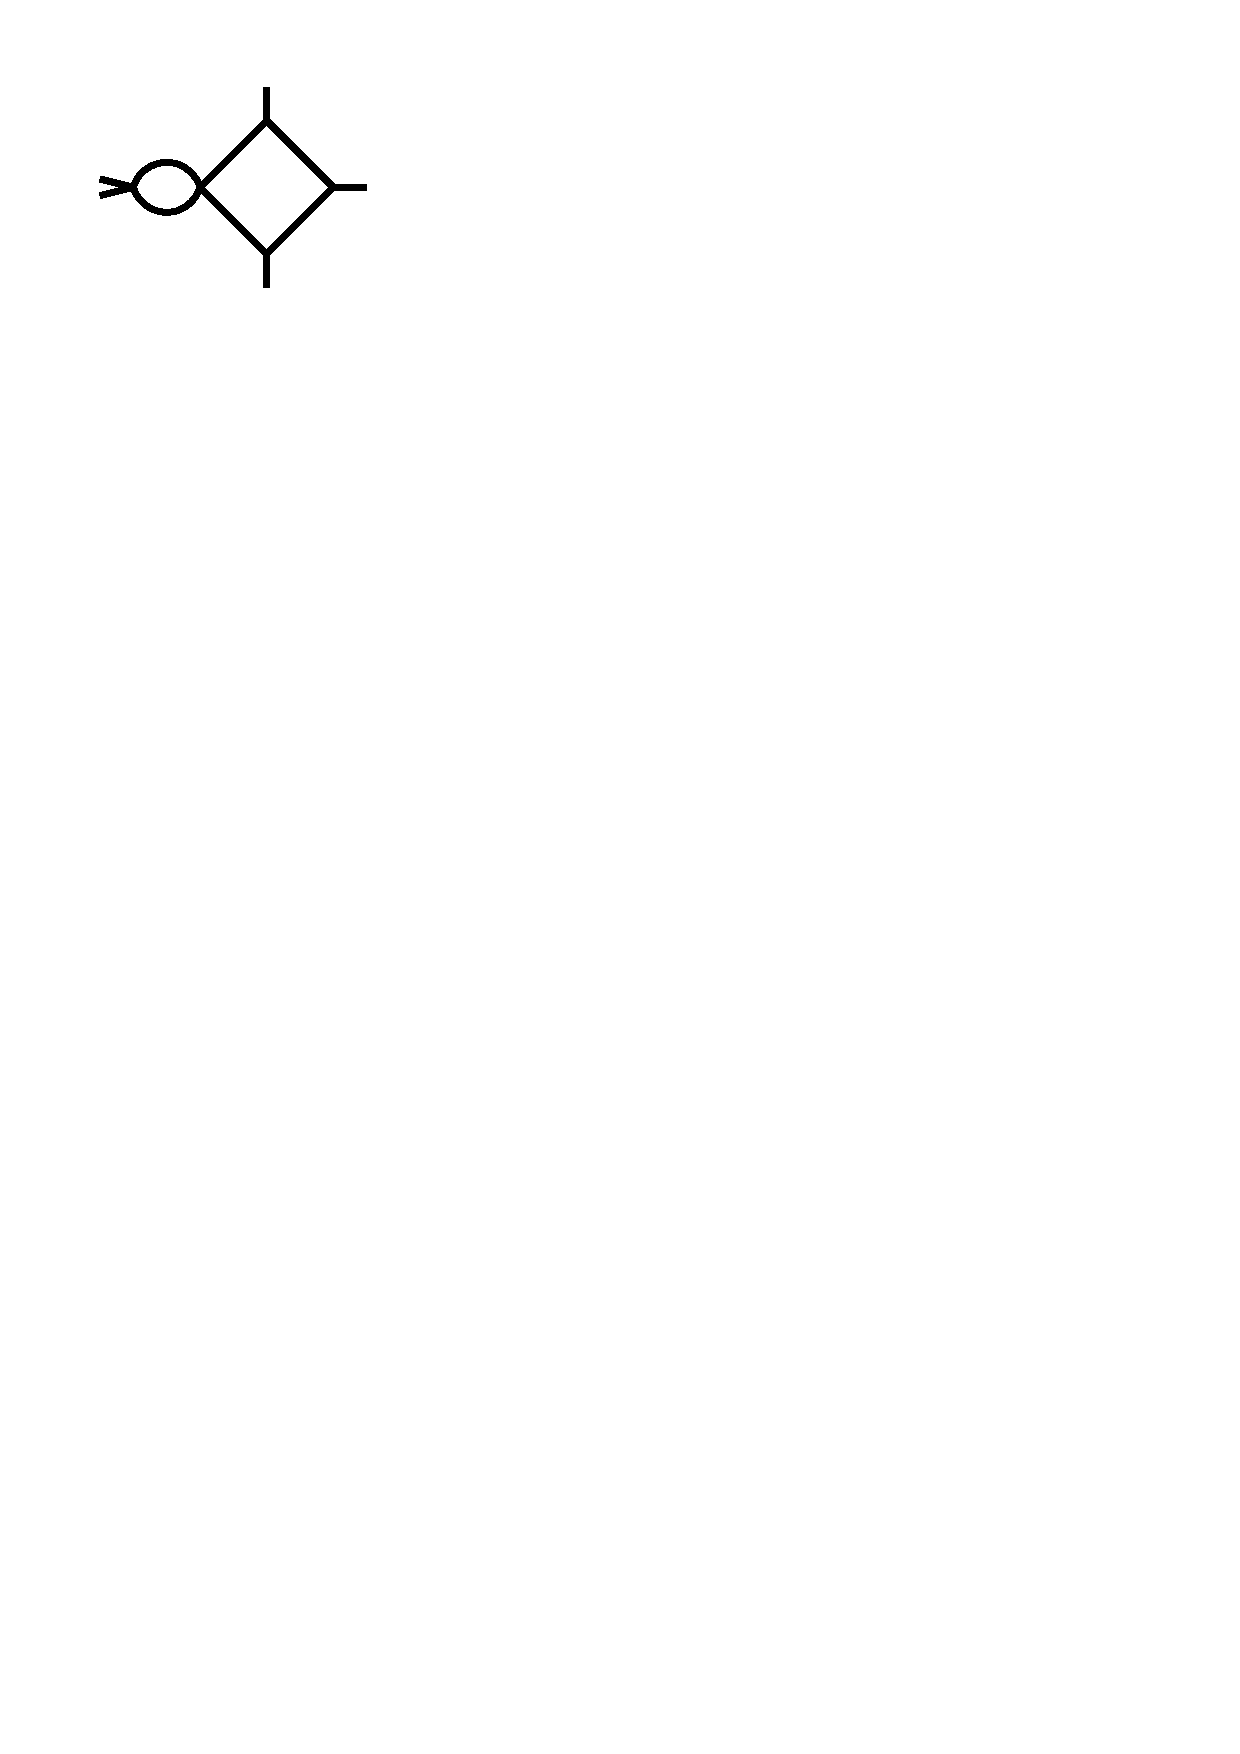
\includegraphics[scale=0.4]{figures/topologies/BoxBubble1LS}};
      \node at
      (5,-9.8){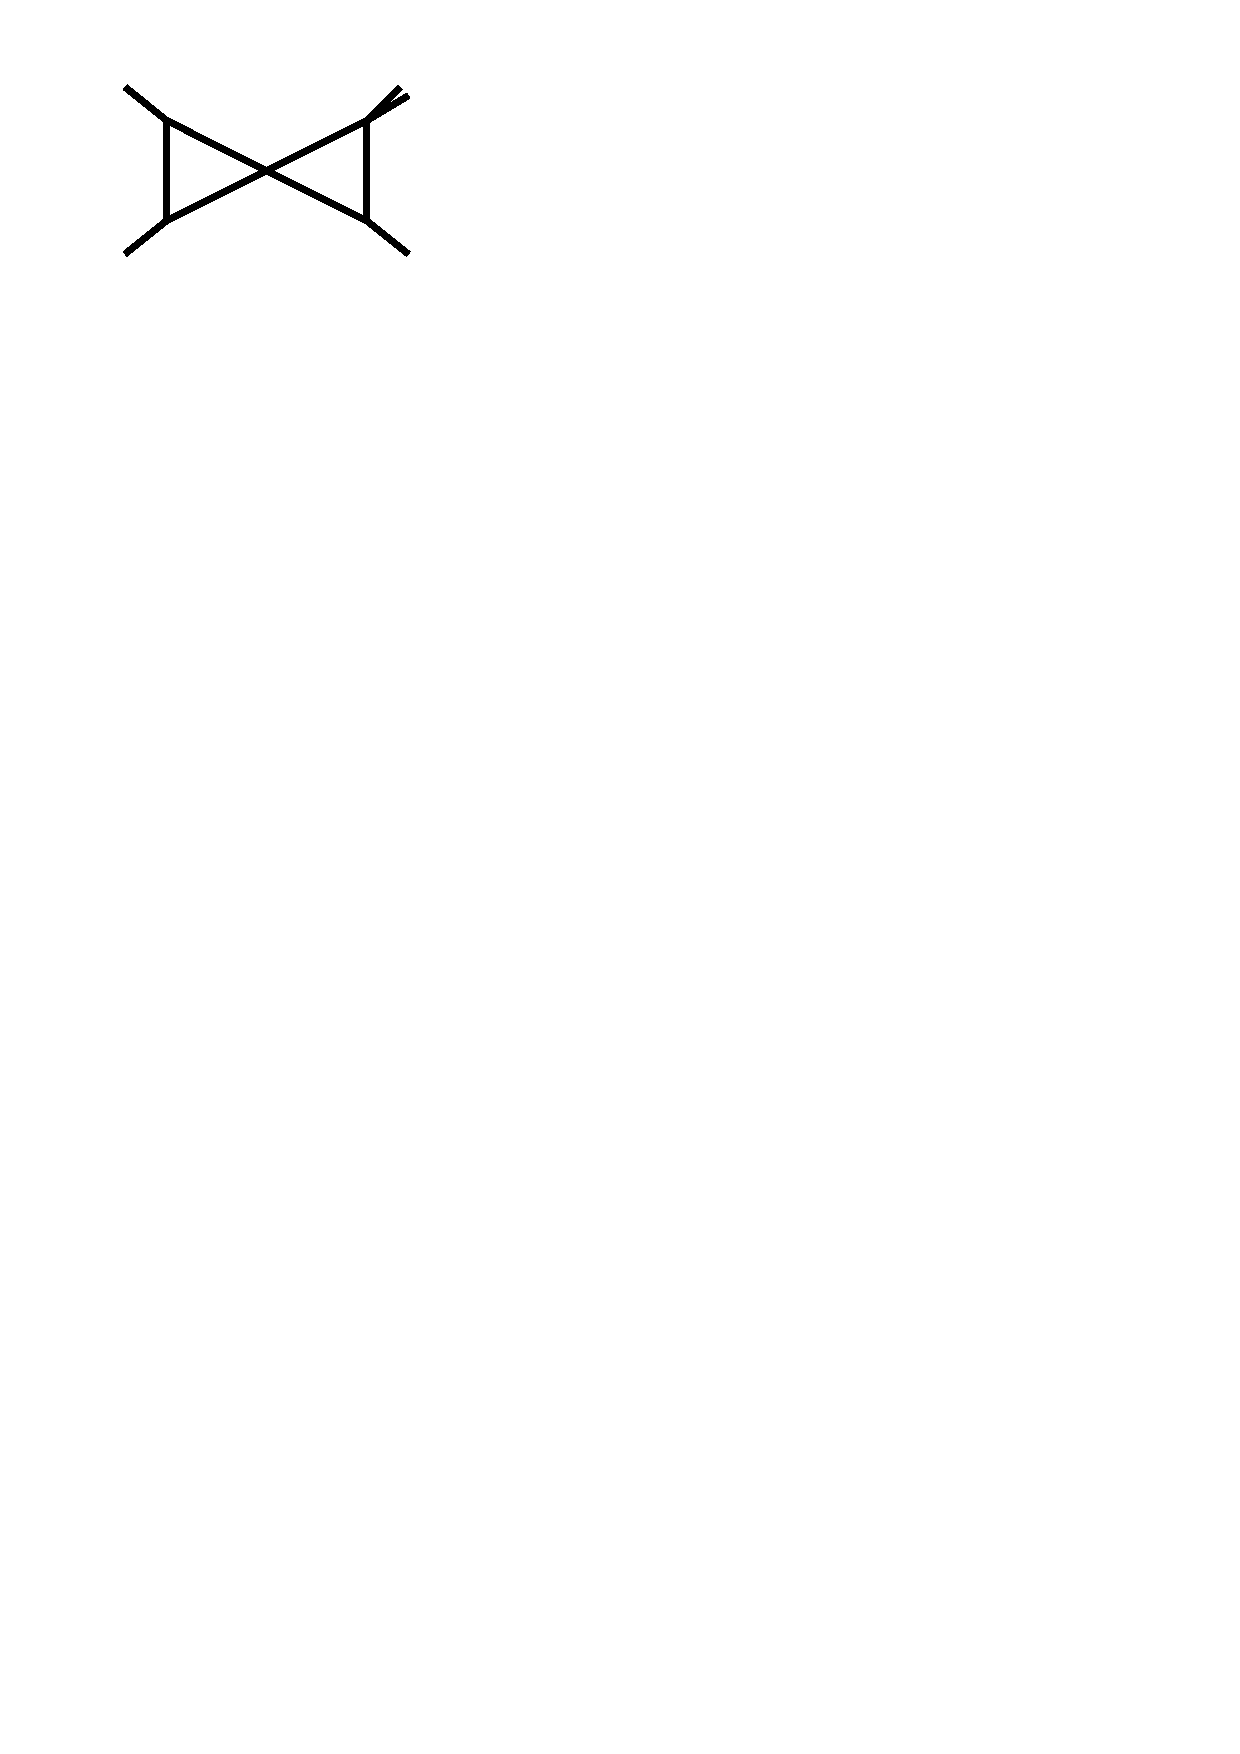
\includegraphics[scale=0.35]{figures/topologies/TriangleTriangle1LS}};
      \node at
      (7,-9.8){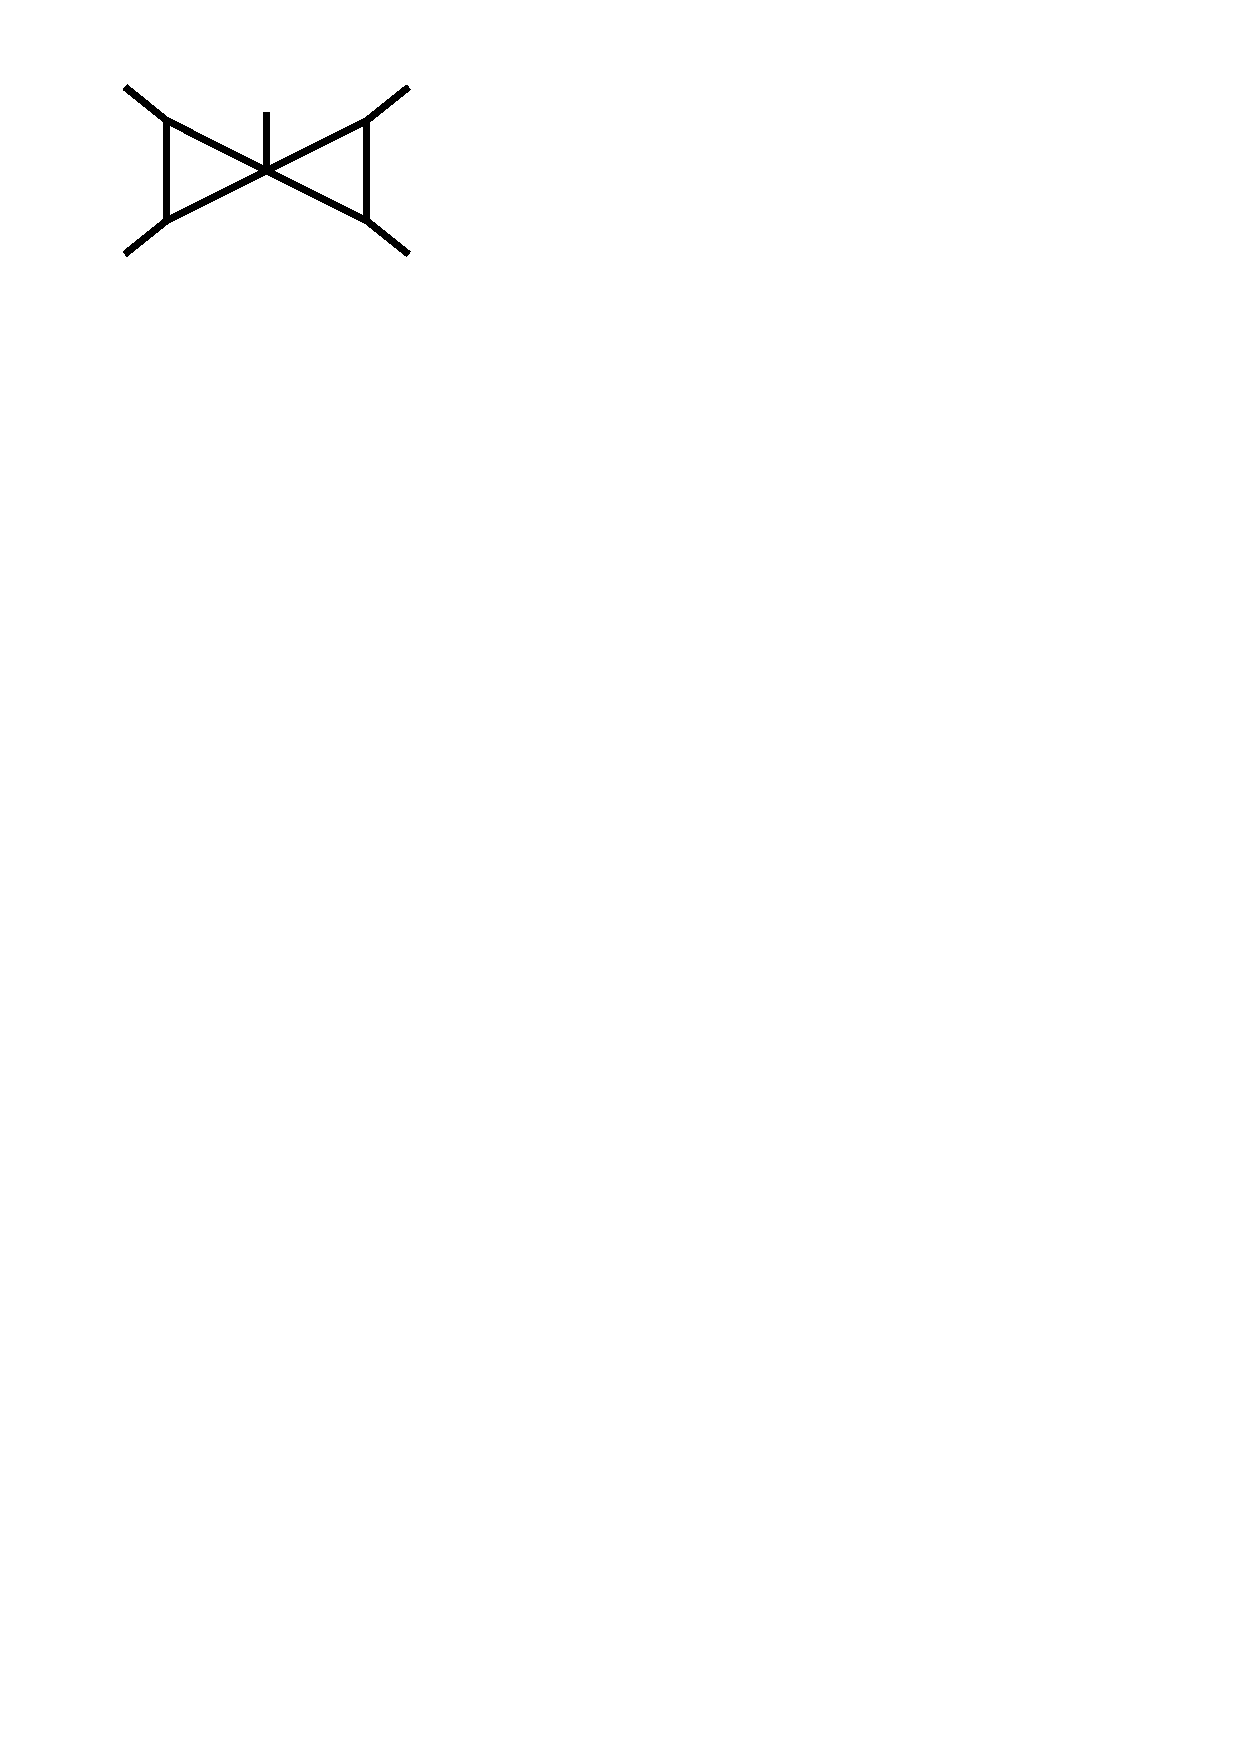
\includegraphics[scale=0.35]{figures/topologies/TriangleTriangle1LSG}};
    % Level 4
      \node at
      (0,-11.5){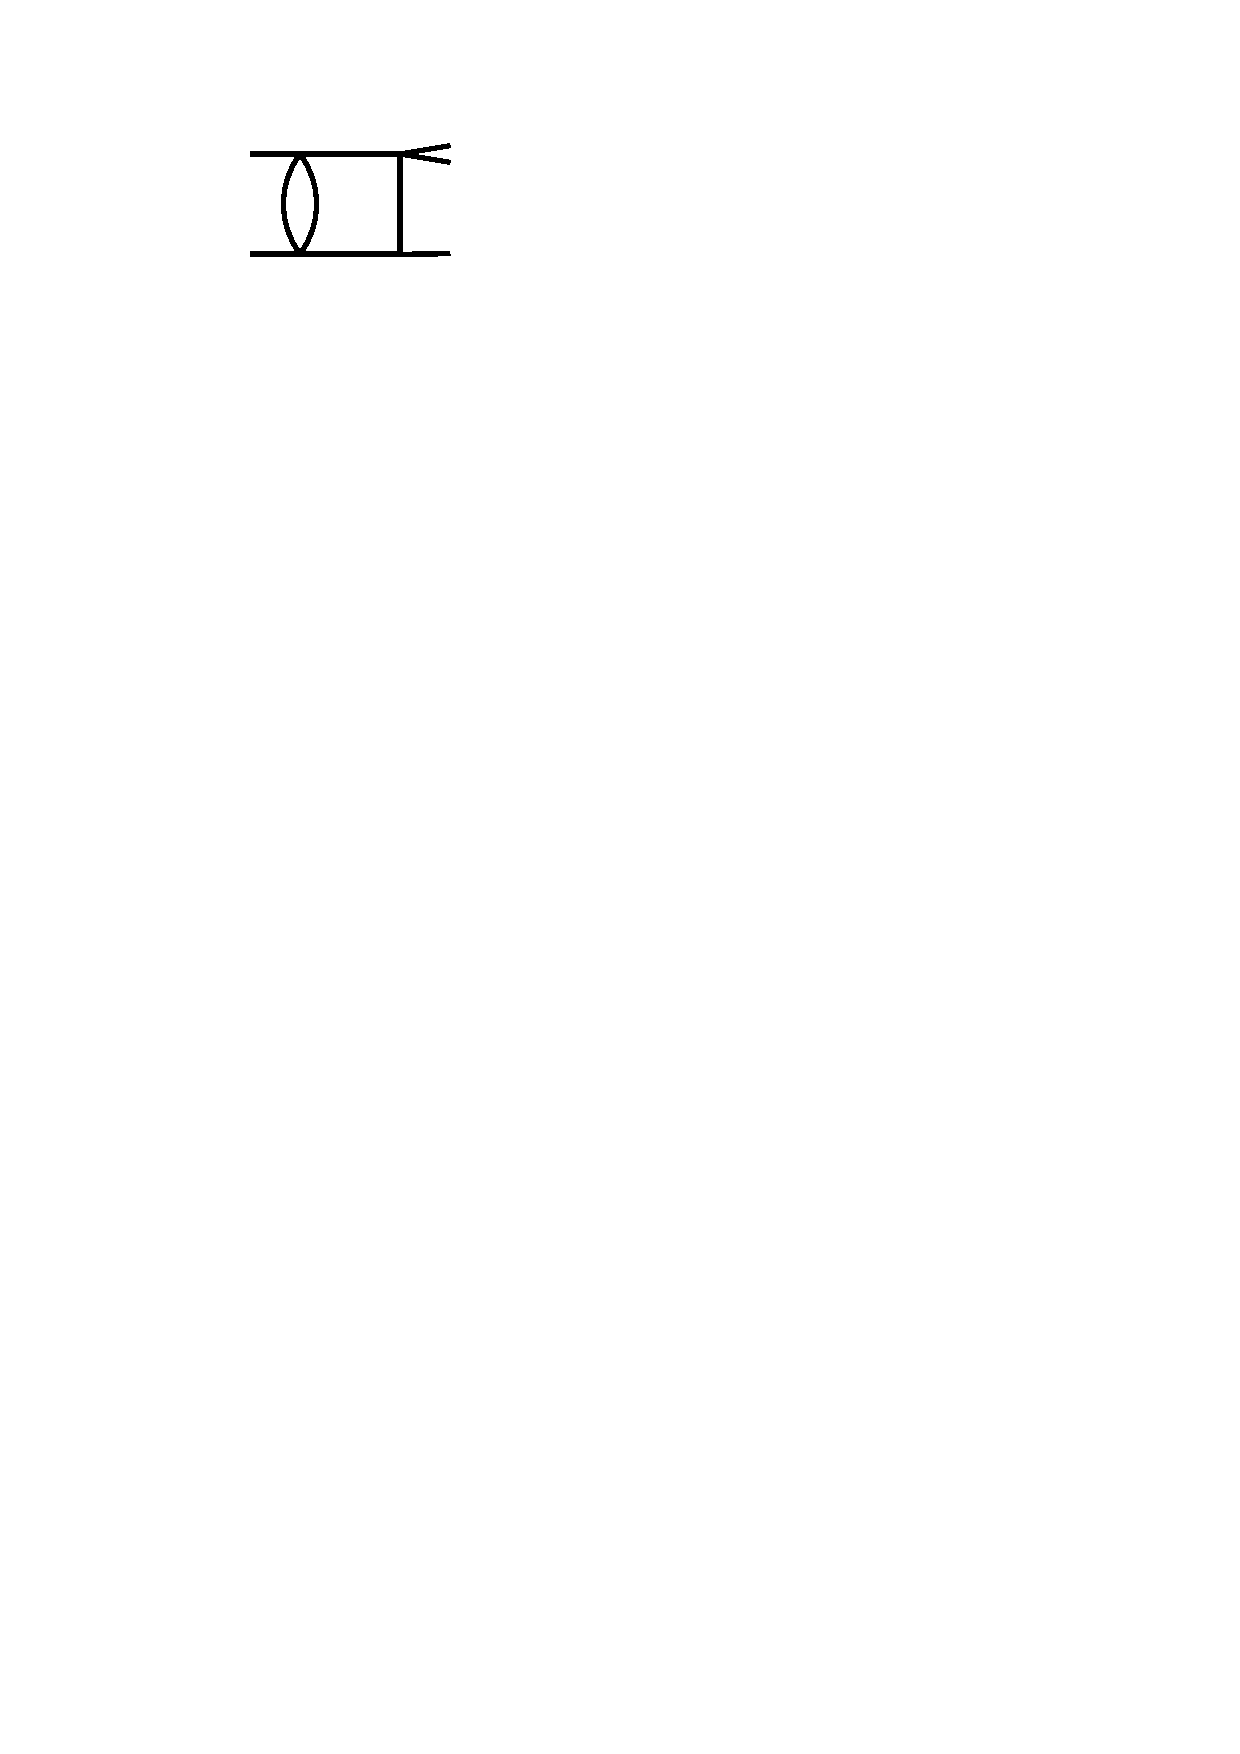
\includegraphics[scale=0.45]{figures/topologies/BoxBubbleGBox}};
      \node at
      (2,-11.5){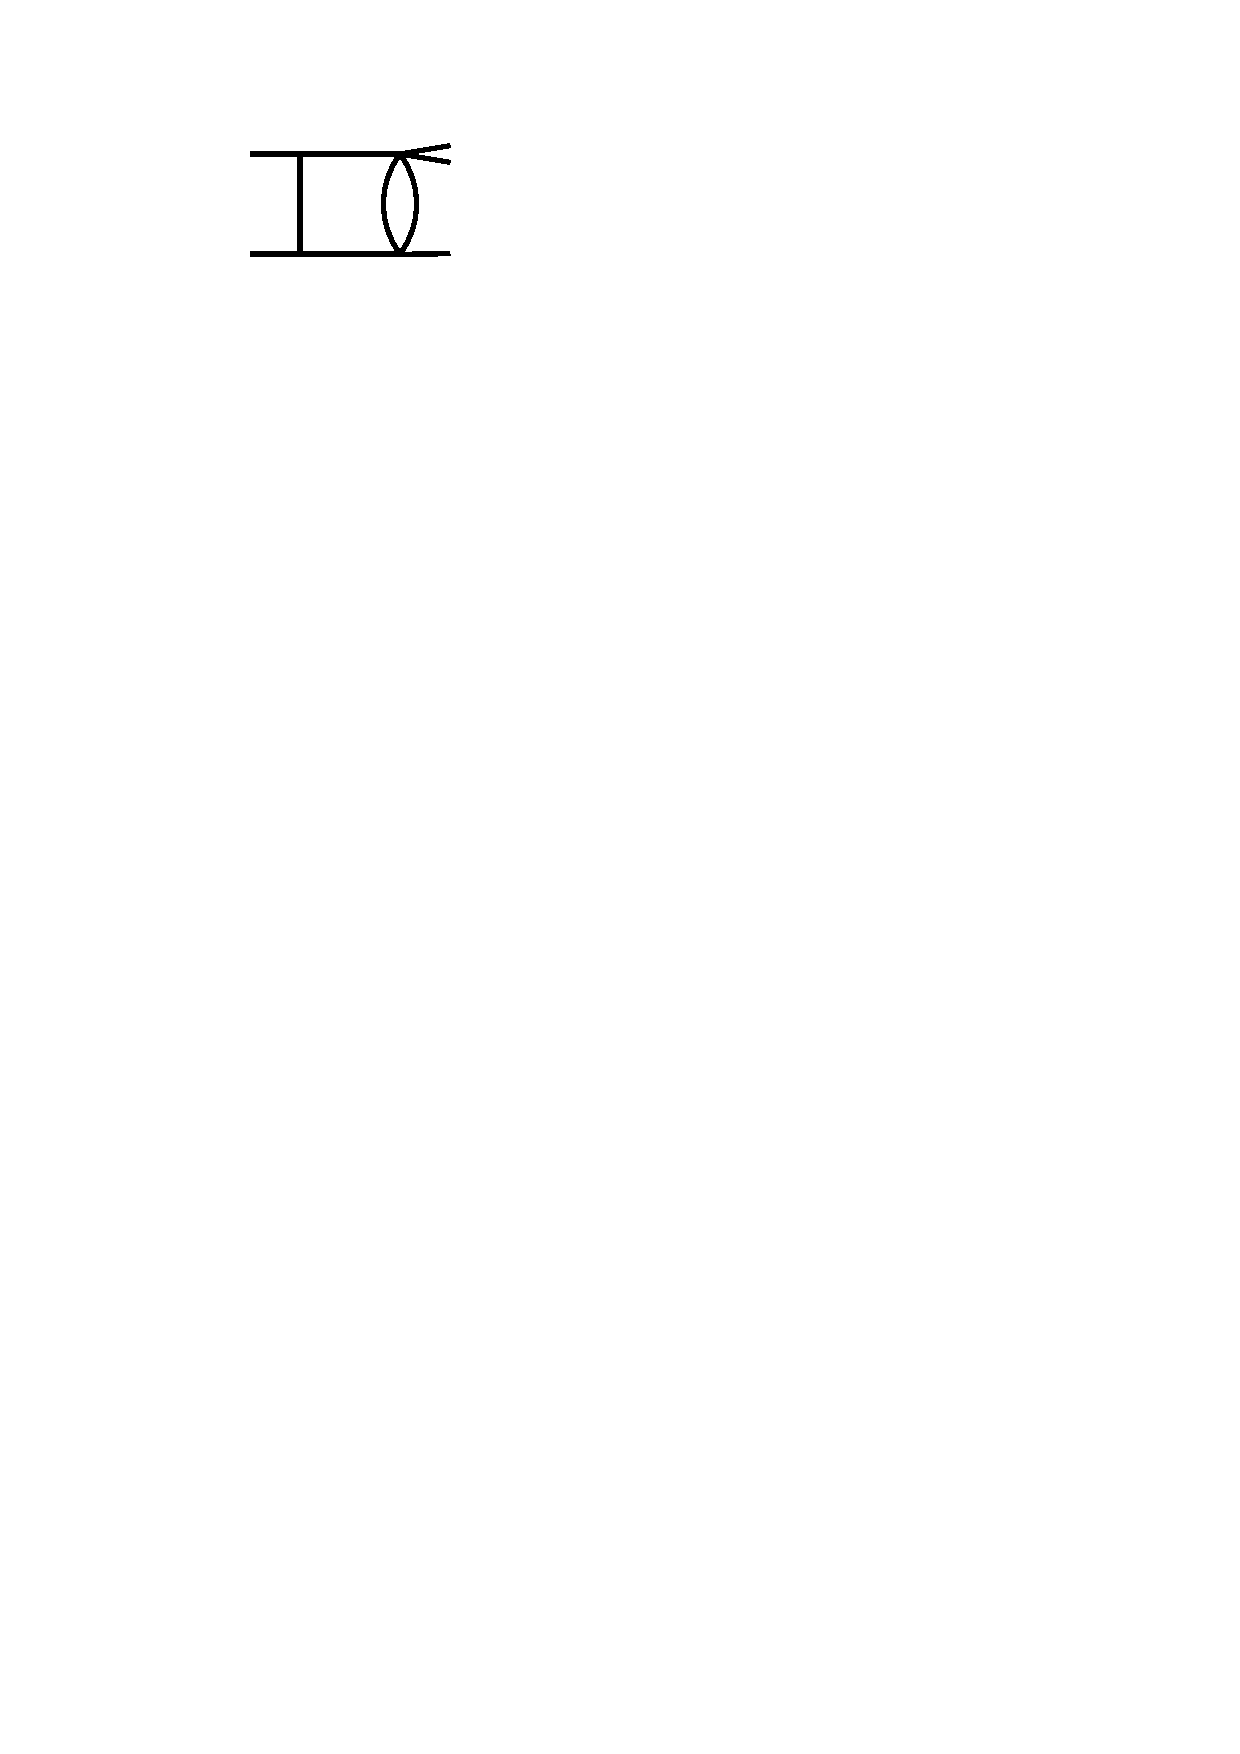
\includegraphics[scale=0.45]{figures/topologies/BoxBubbleGBub}};
      \node at
      (4,-11.5){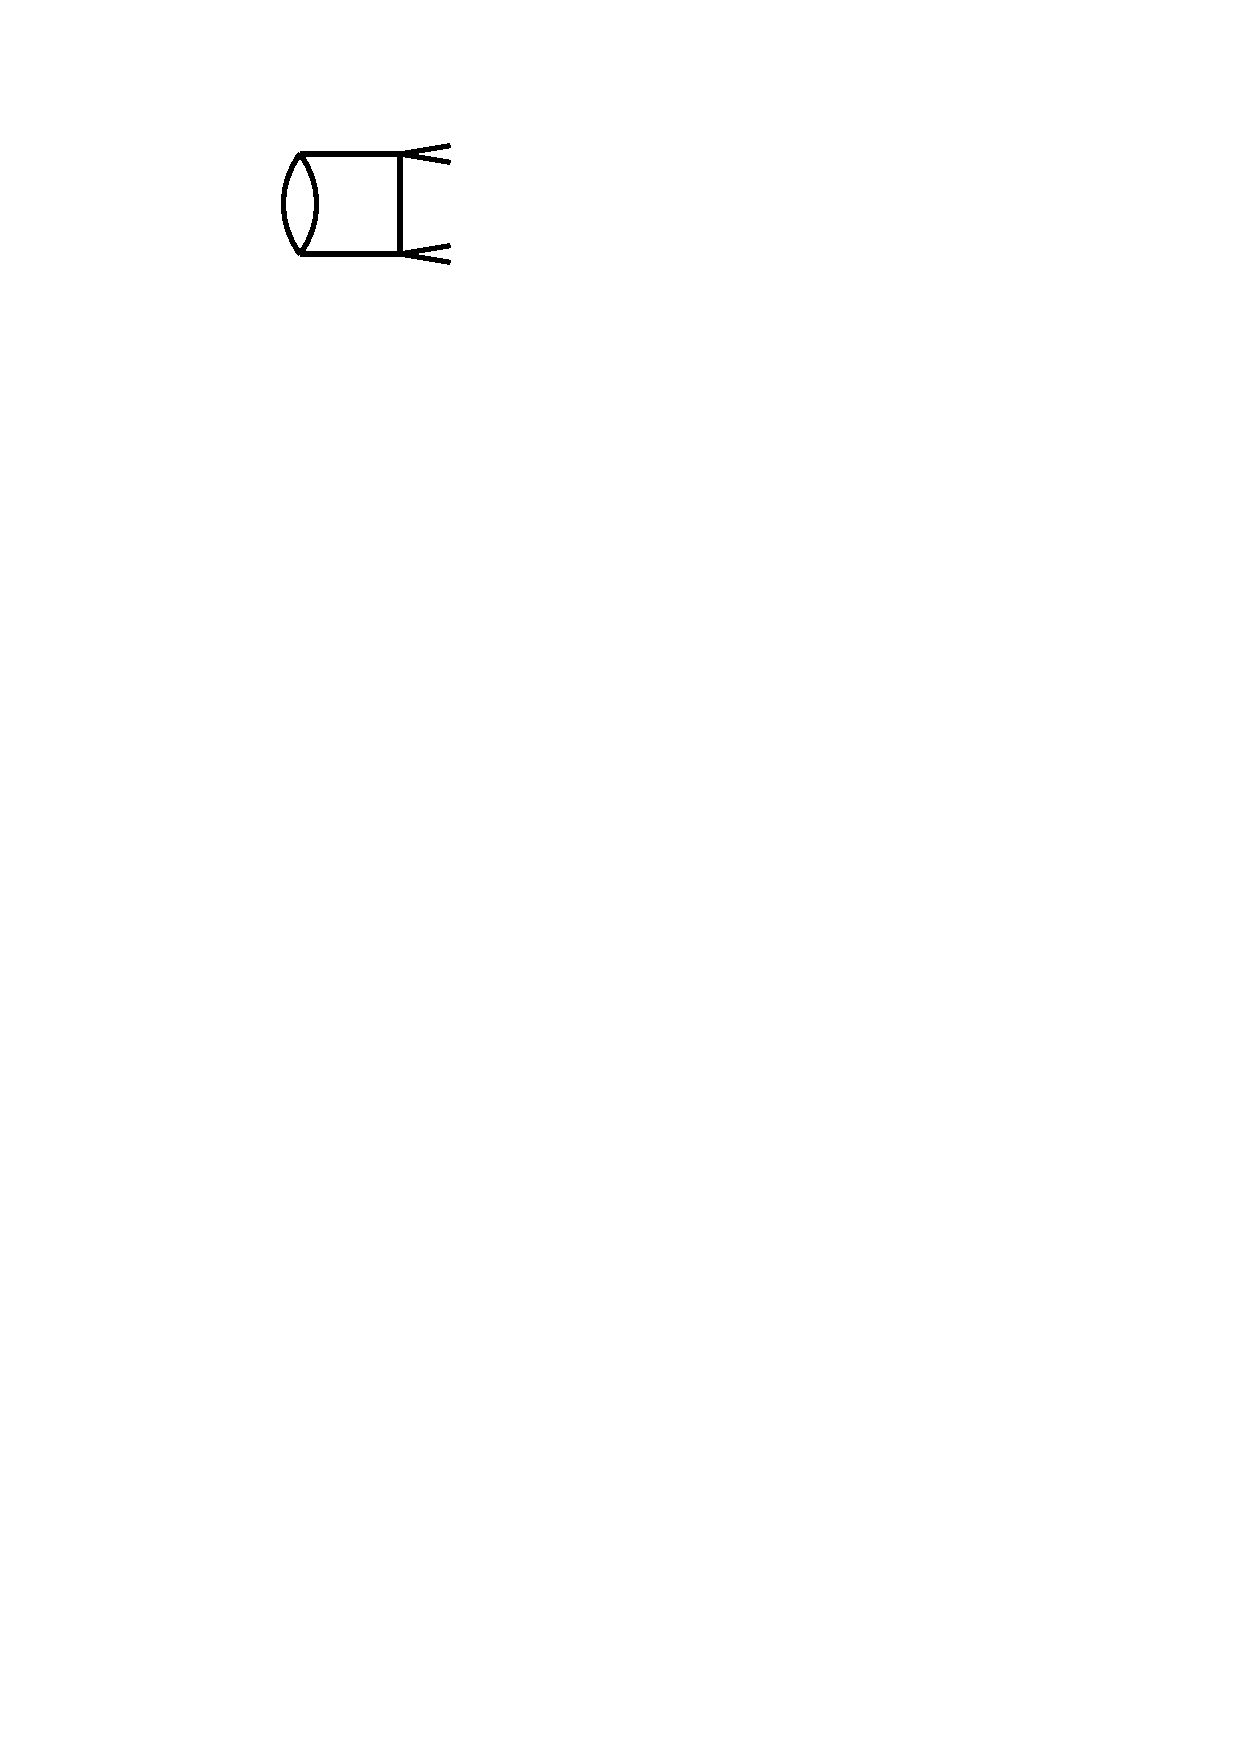
\includegraphics[scale=0.45]{figures/topologies/BoxBubbleRed1}};
      \node at
      (6,-11.5){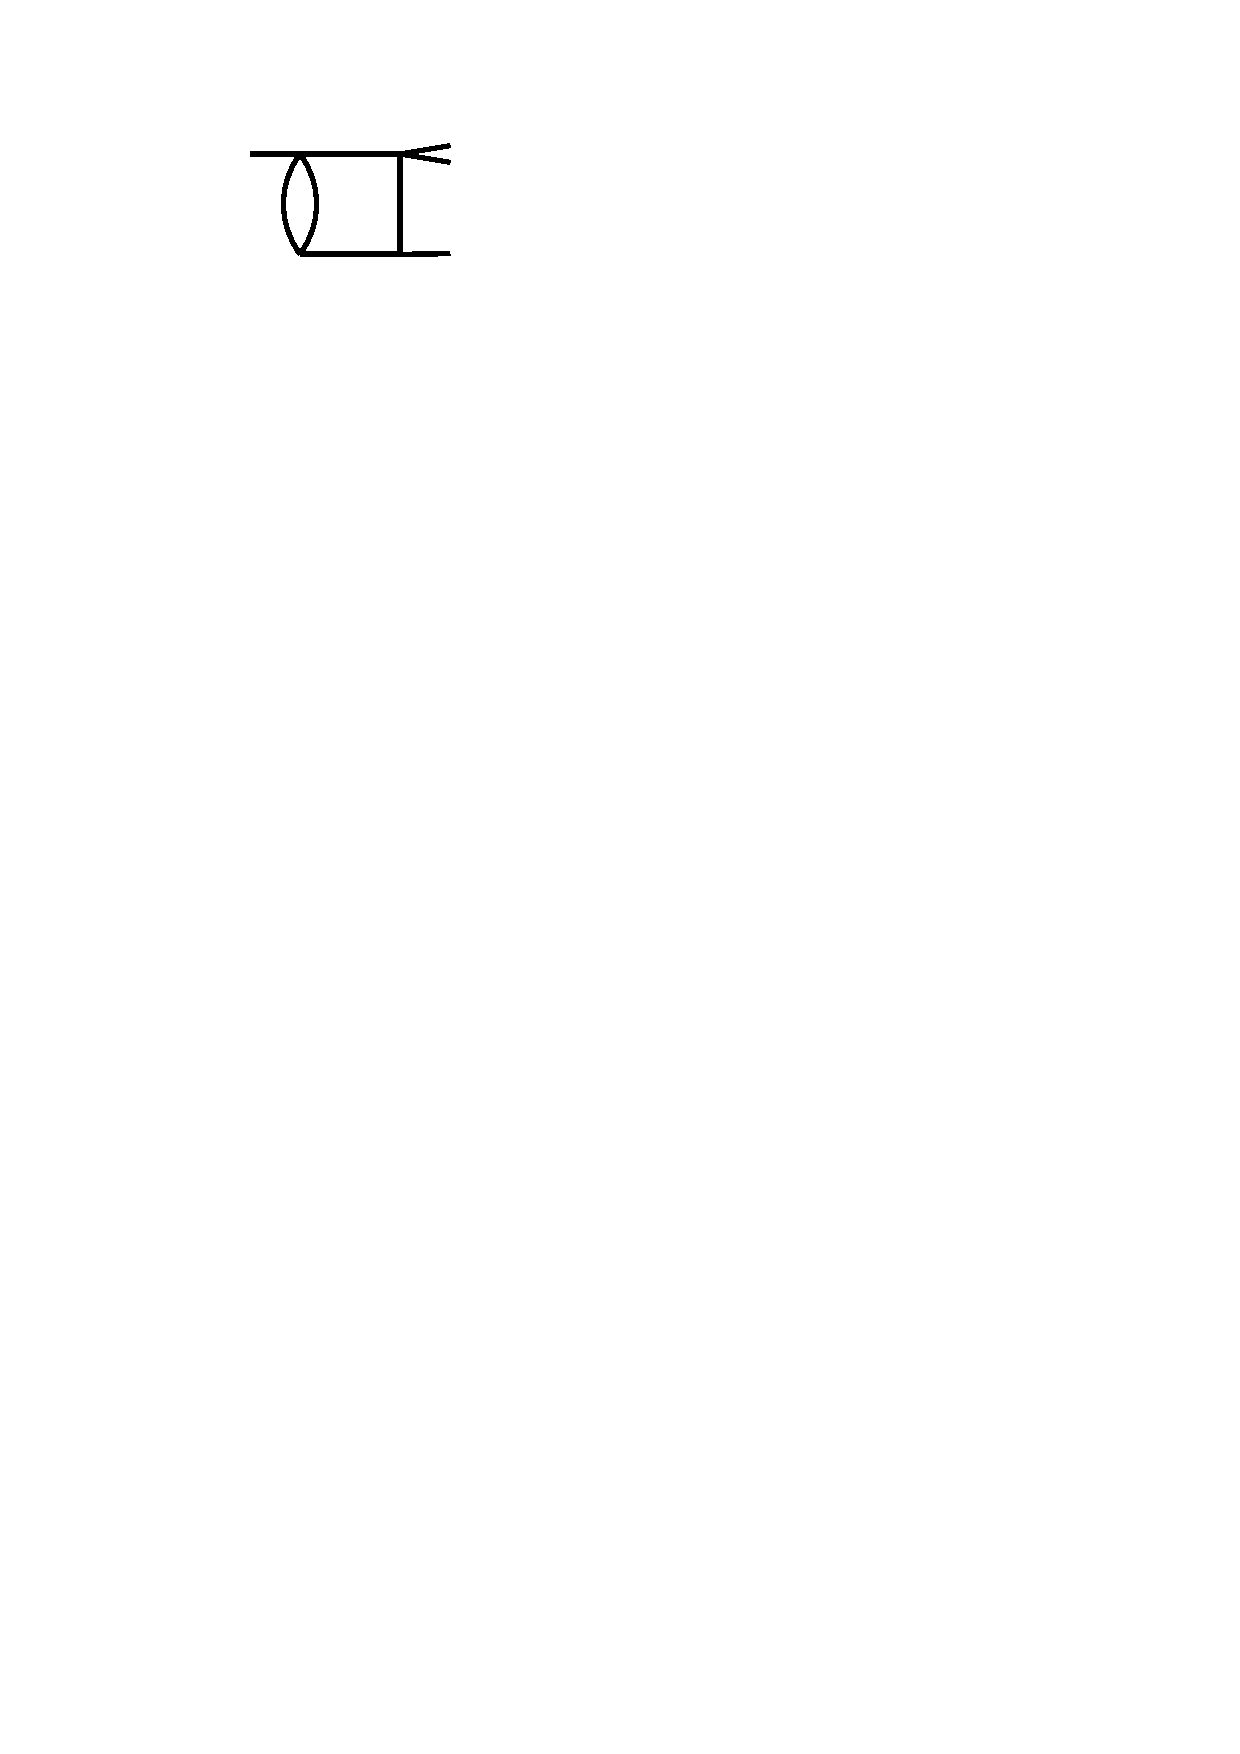
\includegraphics[scale=0.45]{figures/topologies/BoxBubbleRed2}};
      \node at
      (8,-11.5){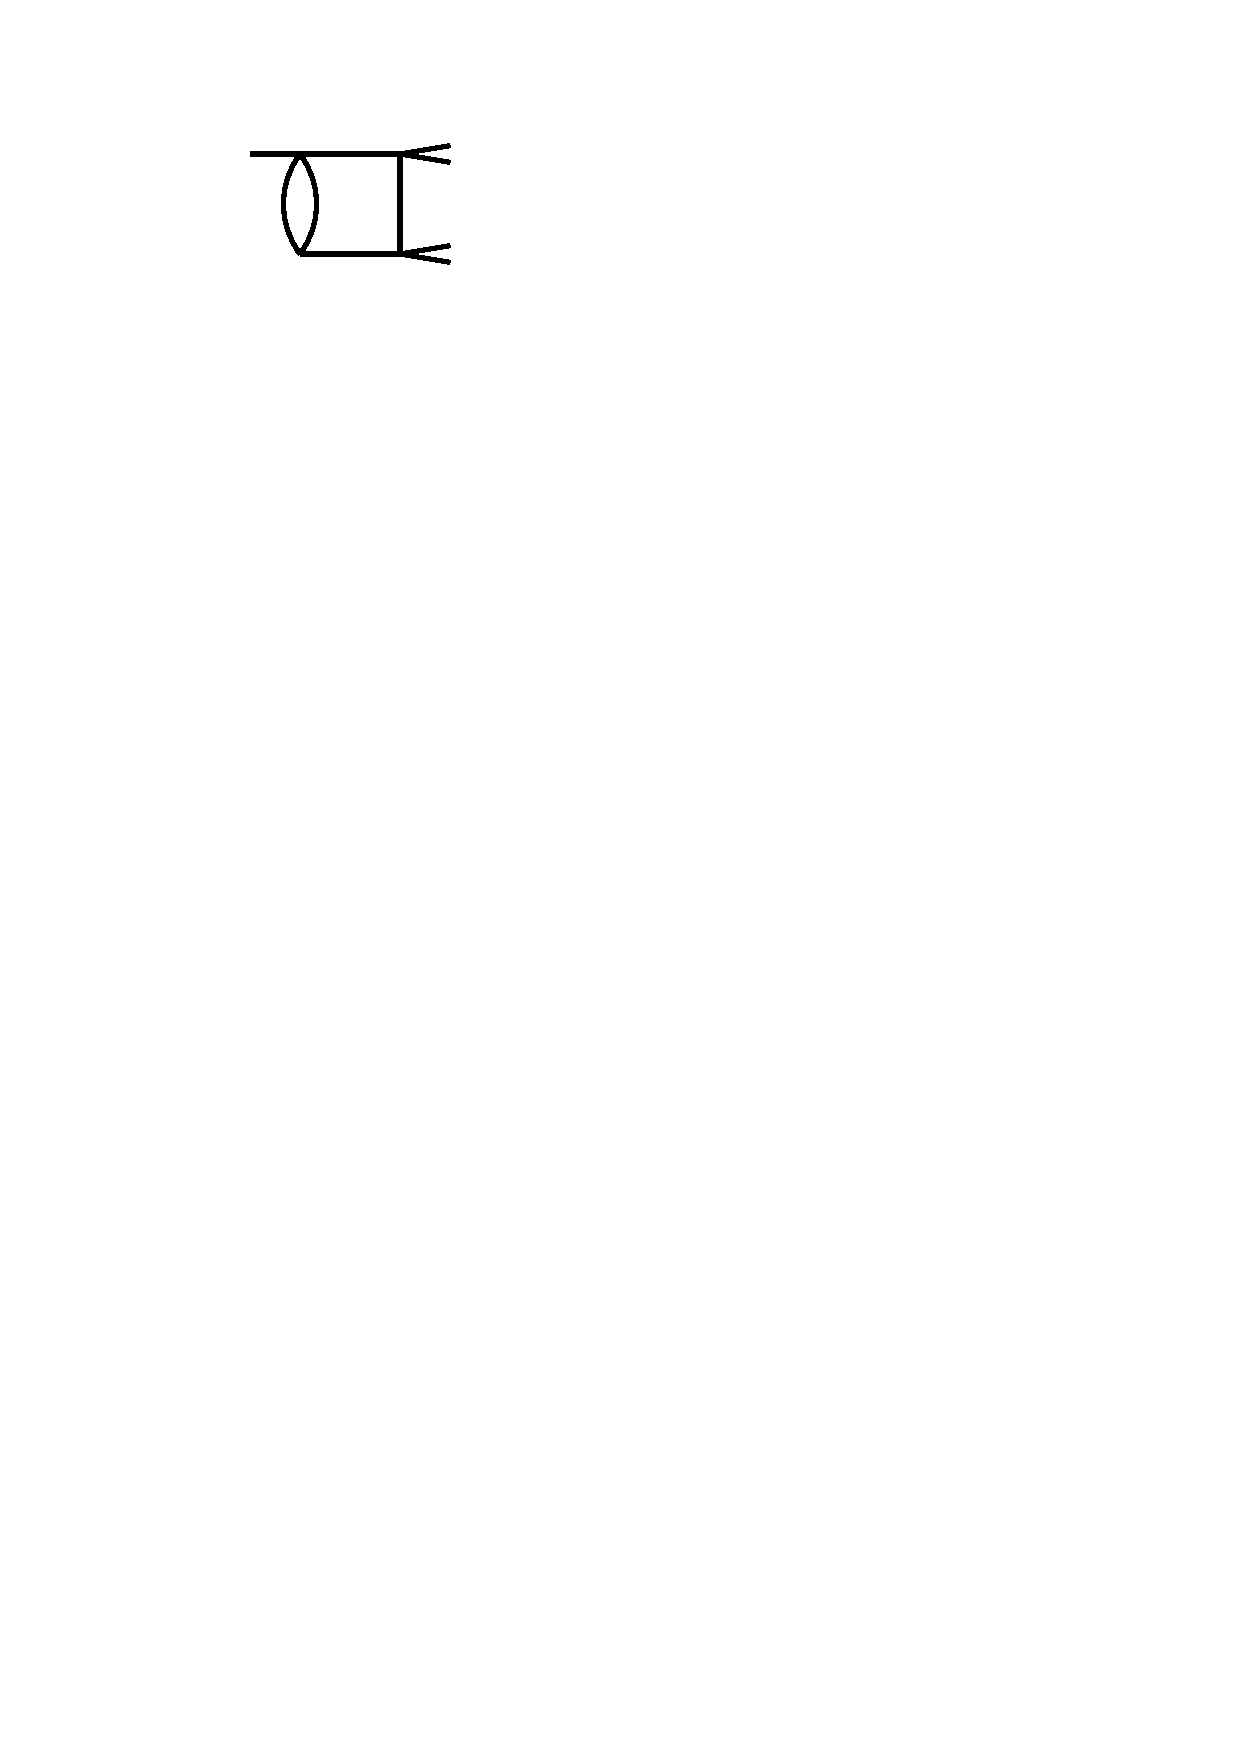
\includegraphics[scale=0.45]{figures/topologies/BoxBubbleRed3}};
      \node at
      (10,-11.5){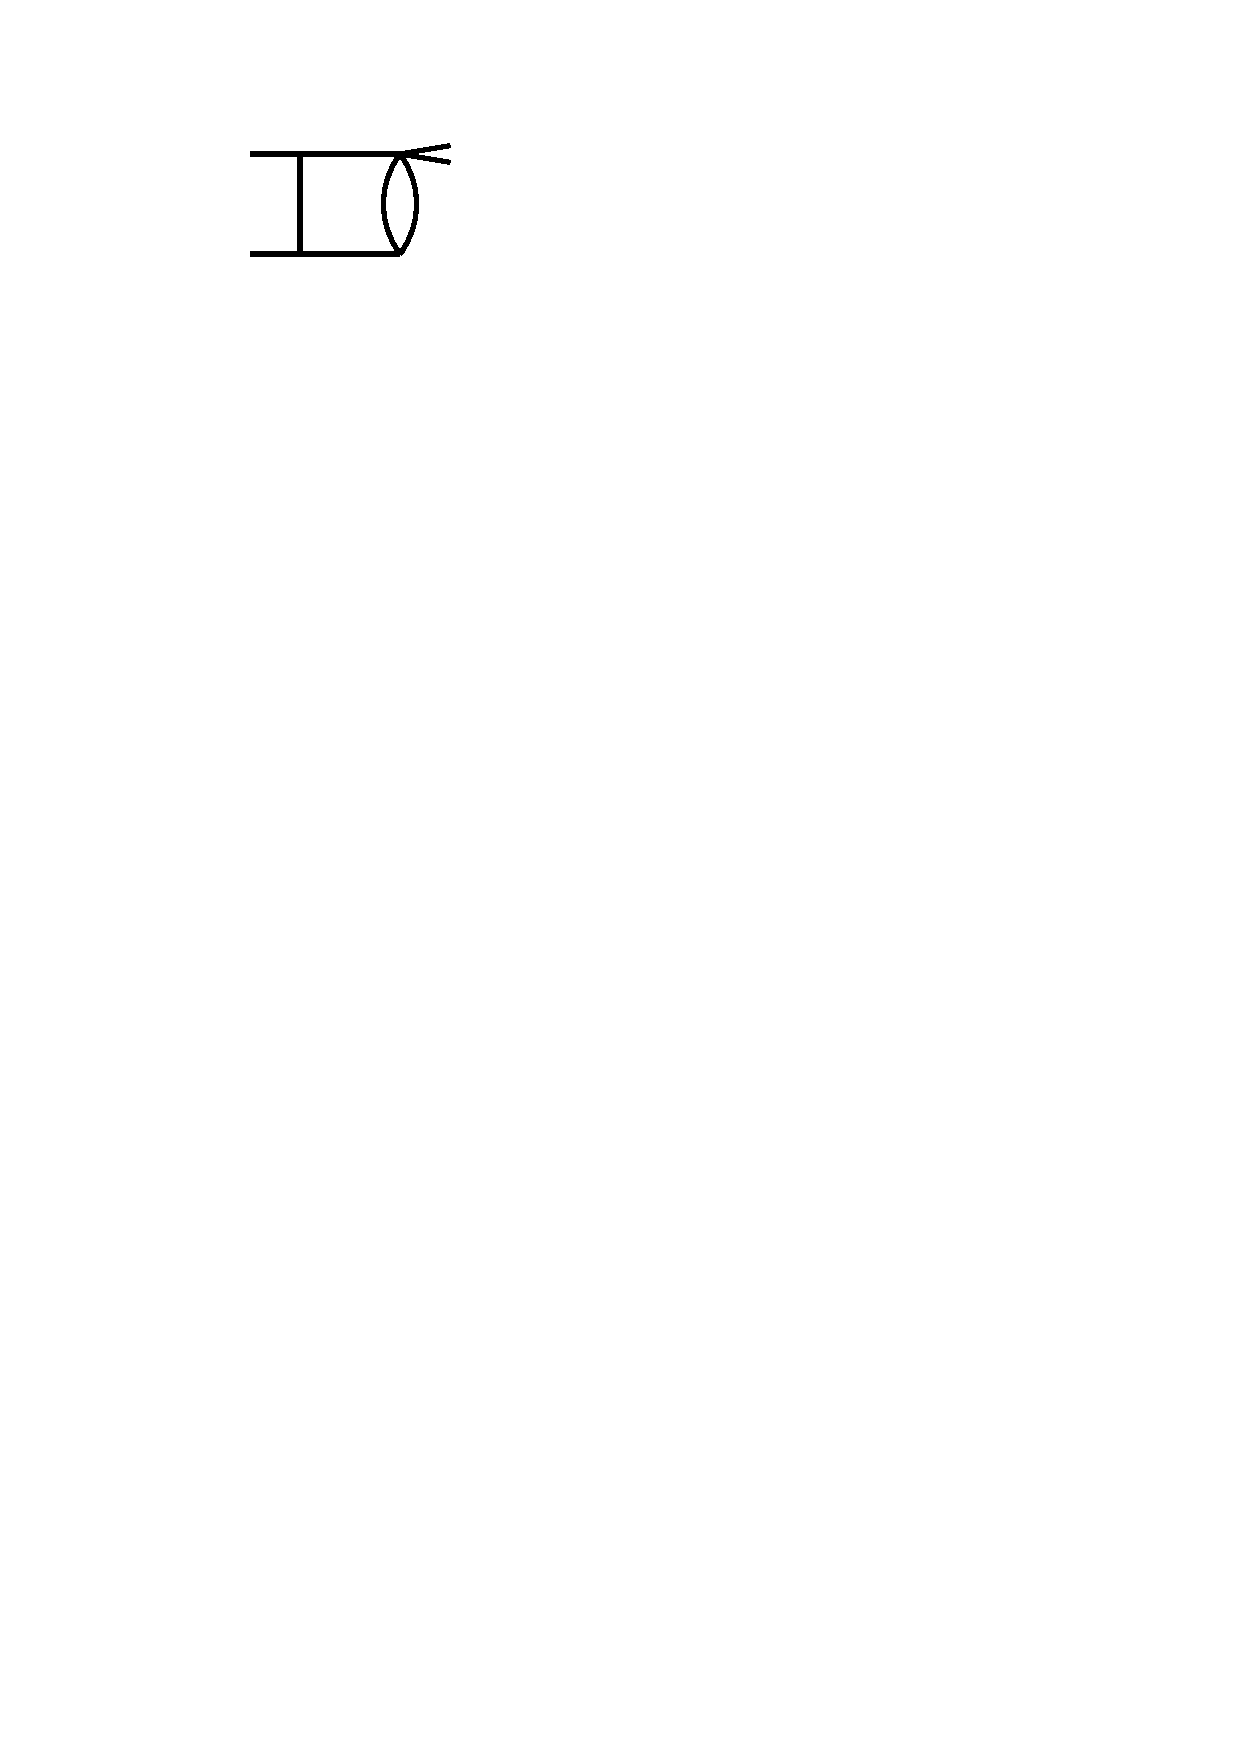
\includegraphics[scale=0.45]{figures/topologies/BoxBubbleRed4}};
    %
      \node at
      (0,-12.7){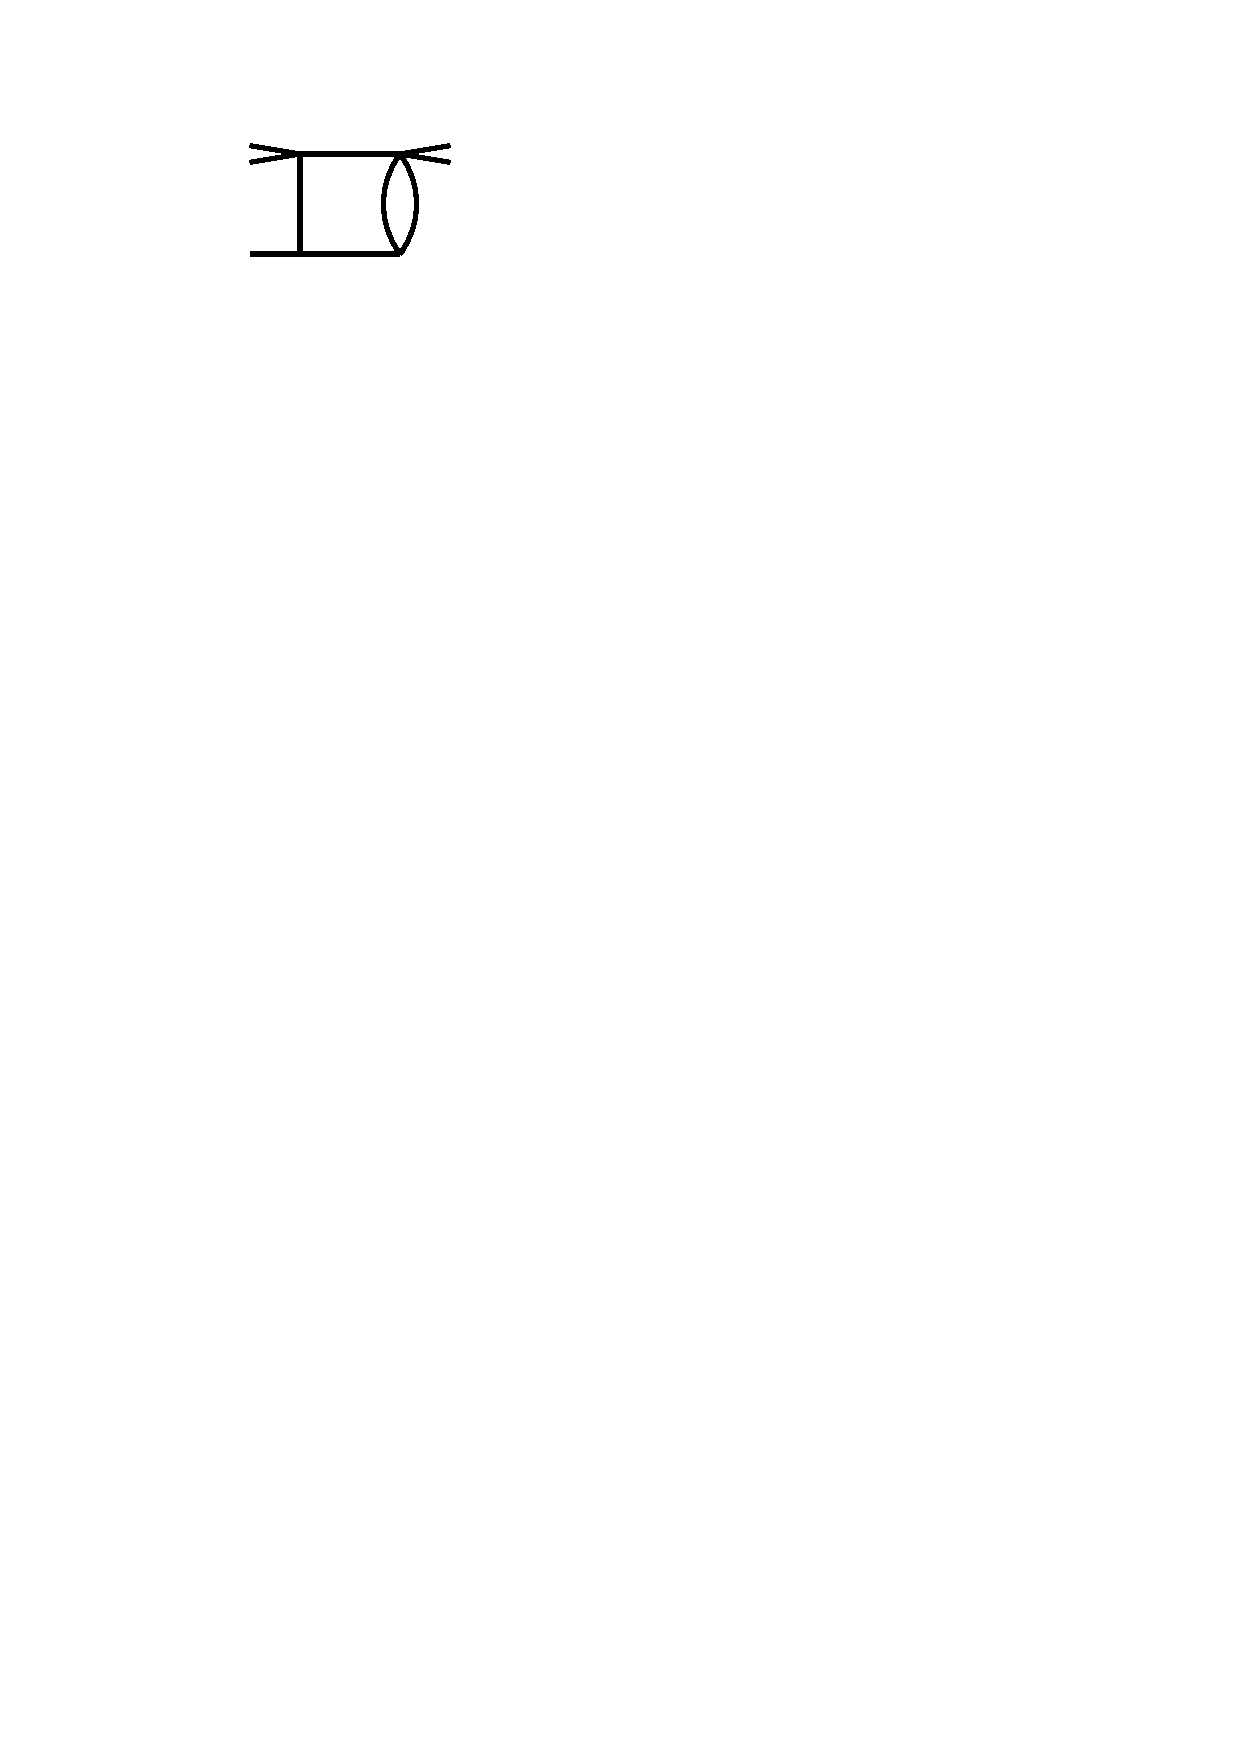
\includegraphics[scale=0.45]{figures/topologies/BoxBubbleRed5}};
      \node at
      (2,-12.7){\includegraphics[scale=0.45]{figures/topologies/BoxBubbleRed6}};
      \node at
      (4,-12.7){\includegraphics[scale=0.45]{figures/topologies/TriangleTriangleGDiag}};
      \node at
      (6,-12.7){\includegraphics[scale=0.45]{figures/topologies/TriangleTriangleGOffDiag}};
      \node at
      (8,-12.6){\includegraphics[scale=0.45]{figures/topologies/TriangleTriangleSG}};
      \node at
      (10.2,-12.75){\includegraphics[scale=0.45] {figures/topologies/TriangleTriangleRed1}};
    %
      \node at
      (0,-13.8){\includegraphics[scale=0.45]{figures/topologies/TriangleTriangleRed2}};
      \node at
      (2.15,-13.8){\includegraphics[scale=0.45] {figures/topologies/TriangleTriangleRed3}};
      \node at
      (4.3,-13.8){\includegraphics[scale=0.45] {figures/topologies/TriangleTriangleRed4}};
      \node at
      (6.45,-13.95){\includegraphics[scale=0.4] {figures/topologies/BubbleTriangle1LS}};
      \node at
      (8.6,-13.95){\includegraphics[scale=0.4] {figures/topologies/BubbleTriangle1LS_2}};
      \node at
      (10.75,-13.95){\includegraphics[scale=0.4] {figures/topologies/BubbleTriangle1LSG}};
    % Level 6
      \node at
      (0,-15.5){\includegraphics[scale=0.5]{figures/topologies/BubbleTriangleG1Mass}};
      \node at
      (1.8,-15.5){\includegraphics[scale=0.5]{figures/topologies/BubbleTriangleG2Mass}};
      \node at
      (3.6,-15.5){\includegraphics[scale=0.5]{figures/topologies/BubbleTriangleSG}};
      \node at
      (5.4,-15.5){\includegraphics[scale=0.5]{figures/topologies/BubbleTriangleRed1}};
      \node at
      (7.2,-15.5){\includegraphics[scale=0.5]{figures/topologies/BubbleTriangleRed2}};
      \node at
      (9,-15.55){\includegraphics[scale=0.5]{figures/topologies/BubbleBubble1LS}};
      \node at
      (10.8,-15.5){\includegraphics[scale=0.5]{figures/topologies/BubbleBubble1LS_2}};
     % Level 7
      \node at
      (5.25,-17){\includegraphics[scale=0.6]{figures/topologies/Sunrise}};
    \end{tikzpicture}
  \end{center}
  \caption{A complete set of topologies appearing in two-loop five-parton scattering, arranged
    in the order of decreasing number of propagators.
    All lines are massless, with massive external legs being denoted by two massless external lines entering a vertex.
    The figure is taken from \cite{Abreu:2017hqn}.
  }
  \label{fig:PropagatorStructures}
\end{figure}
%%%%%%%%%%%%%%%%%%%%%%%%%%%%

\subsubsection{Hierarchies and Color Decomposition}

We now describe how do we organize the amplitudes into a set of cut equations \cref{eq:cut_equations} for master/surface coefficients.

First we generate all cut diagrams contributing to the amplitude with \textsc{QGRAF} \cite{Nogueira:1991ex}.
To obtain the \emph{cut diagrams}, instead of Feynman diagrams,
we list all possible tree amplitudes as allowed vertices in the model files,
and request the one-particle-irreducible diagrams only.

We then process these diagrams with a custom  \texttt{Mathematica} code, which performs three steps:
\begin{enumerate}
  \item Organize the cut diagrams into the hierarchy (see \cref{eq:topology_order,eq:topology_sequence}) 
    This amounts to constructing a layered tree graph with vertices as nodes,
    and the relation of adding/removing propagators as edges.
  \item Color decomposition into partial amplitudes.
  \item Decomposition of each cut diagram into polynomials in $(D_s-6)$, as described in \cref{dshel:sec:unitarity-compatible}.
\end{enumerate}
In principle, the order of these steps is irrelevant.
The purpose of color decomposition is to separate the color factors from the rest of the computation, 
such that  the partial amplitudes (see \cref{5parton:sec:color_structures}) are evaluated in terms of color-stripped Feynman rules of \cref{sec:cofr}.
Our color decomposition is based on \cite{Ochirov:2016ewn,Ochirov:2019mtf},
and is accomplished in the same ``unitarity-compatible'' spirit of the algorithm discussed in \cref{dshel:sec:unitarity-compatible}.
We process each cut diagram separately in the following way:
\begin{enumerate}
  \item Decompose each of it's vertices (i.e.\ tree amplitudes) into linear combinations of color-ordered tree amplitudes multiplied by color factors.
  \item Insert the decompositions from the previous step into the diagram and expand.
  \item Contract all internal color indices through the cut propagators, and perform the color algebra
  \item Collect the terms with the same color factor, $N_c$, and $N_ f$ powers. 
\end{enumerate}
In this way, we find all terms contributing to the partial amplitudes,
and, by construction, the tree amplitudes in the corners of all cut diagrams are color-ordered tree amplitudes.


\subsubsection{Color-Stripped Cuts}
The products of tree amplitudes in cut diagrams contributing to the partial amplitudes are evaluated
numerically with the custom \texttt{C++} implementation of the off-shell recursion, as described in \cref{sec:evaluation_of_cuts}.
We have implemented evaluations both in multi-precision floating-point arithmetic, and over finite fields with cardinalities of the order $2^{31}$.
For the former we use the QD \cite{QD} library. And for the latter we use \texttt{Givaro} \cite{Givaro} with 
custom optimizations of multiplications through Barrett reduction \cite{Barrett1987a,Hoeven2014}.
The finite-filed evaluations are crucial for the reconstruction of the analytic expressions.

In the off-shell recursion we use explicit components of six-dimensional loop momenta 
satisfying the cut conditions (see \cref{sec:osm} for details). 
This has an important implication for the evaluations over finite fields, where
we cannot take square roots originating from the quadratic equations.
We workaround this complication by allowing the off-shell currents to
take values in an algebraic extension of the finite field.
We consider this in more detail in \cref{sec:muij_square_roots}.
However, since the cuts of properly defined (normalized) helicity amplitudes are Lorentz scalars,
we can still solve the cut equations \eqref{eq:cut_equations} in non-extended finite fields.
For the same reason, the signature of the metric tensor is non-essential, as long as values 
of the invariants do not change. This allows us to employ the alternating metric signature $\{+,-,+,-,\ldots{}\}$
and avoid the usage of complex numbers whatsoever, which represents a significant optimization.

We solve the linear systems of equations for the coefficients with a custom implementation of PLU factorization and back substitution
when working with finite fields. In floating-point arithmetic we solve the equations with the QR factorization,
as implemented in \texttt{Eigen} \cite{eigen}.




\section{Numerical Results}
\label{sec:5parton:numerics}

In this section, we provide the numerical benchmark values for a full set of  five-parton two-loop helicity amplitudes.
For completeness we also provide the values  of the corresponding one-loop amplitudes to $\order{\eps^2}$.
We also provide the values of the four-parton two-loop amplitudes, which we used for the validation.

The partial two-loop helicity amplitudes are represented in terms of master integrals $I_{\Gamma,i}$ (see \cref{fig:MasterInt}) as
\begin{equation} \label{eq:ampl_master_integrals}
  \mathcal{A}^{(2)}=\sum_{\Gamma\in\Delta}
  \sum_{i\in M_\Gamma} c_{\Gamma,i}\,
  \mathcal{I}_{\Gamma,i}\,,
  \quad
    \qquad I_{\Gamma,i} =
      \qty(\int \prod_{i=1}^{L} \tilde{\dd{\ell_i}}) \frac{m_{\Gamma,i}}{\prod_{j\in P_\Gamma} \rho_j^{\gamma_{\Gamma i,j}}},
\end{equation}
and we obtain the master coefficients as explained in great detail above.
The master integrals are computed as a Laurent series in $\eps$, 
%The master integrals for planar five-parton amplitudes has been computed in \cite{Papadopoulos:2015jft,Gehrmann:2018yef}.
with the coefficient of each power evaluated to linear combinations of multiple polylogarithms (MPLs). 
We now also expand the master-integral coefficients (which are rational functions of $D=4-2\eps$) in a Laurent series in $\eps$.
To obtain the numerical values of the amplitudes we employ two different choices of master integrals.
In both cases we will limit ourselves to the \emph{Euclidian} region, which for the case of five-parton
amplitudes corresponds to all invariants being negative. In \cite{Gehrmann:2018yef} the analytic
continuation to all physical regions has been carried out, so it is rather straightforward to extend
our results to these regions.\footnote{
  Note that our method of obtaining master-integral coefficients is indifferent to the choice of the region.
}

\begin{figure}[ht] 
  \begin{center}
    \begin{tikzpicture}[scale=1.2]
    % 5 point masters
      \node at (5,0){\includegraphics[scale=0.4]{figures/topologies/BoxPentagon}};
      \node at (5,-1){3 masters};
    % Level 2 
      \node at
      (2.5,-1.5){\includegraphics[scale=0.4]{figures/topologies/BoxBoxSG}};
      \node at (2.5,-2.3){3 masters};
      \node at
      (7.5,-1.6){\includegraphics[scale=0.4]{figures/topologies/BoxBox}};
      \node at (7.5,-2.3){2 masters};
    % Level 3
      \node at
      (0.5,-3.3){\includegraphics[scale=0.35]{figures/topologies/BubblePentagonG}};
      \node at (0.5,-4.1){2 masters};
      \node at
      (3.5,-3.3){\includegraphics[scale=0.4]{figures/topologies/BoxTriangleG}};
      \node at (3.5,-4.1){2 masters};
      \node at
      (6.5,-3.2){\includegraphics[scale=0.4]{figures/topologies/BoxTriangleSG}};
      \node at (6.5,-4.1){1 master};
      \node at
      (9.5,-3.3){\includegraphics[scale=0.4]{figures/topologies/BoxBubble1LS}};
      \node at (9.5,-4.1){1 master};
    % Level 4
      \node at
      (0,-4.9){\includegraphics[scale=0.45]{figures/topologies/BoxBubbleGBox}};
      \node at (0,-5.7){1 master};
      \node at
      (2.5,-4.9){\includegraphics[scale=0.45]{figures/topologies/BoxBubbleGBub}};
      \node at (2.5,-5.7){1 master};
      \node at
      (5,-4.9){\includegraphics[scale=0.45]{figures/topologies/TriangleTriangleGDiag}};
      \node at (5,-5.7){1 master};
      \node at
      (7.5,-4.9){\includegraphics[scale=0.45]{figures/topologies/TriangleTriangleGOffDiag}};
      \node at (7.5,-5.7){2 masters};
      \node at
      (10,-4.8){\includegraphics[scale=0.45]{figures/topologies/TriangleTriangleSG}};
      \node at (10,-5.6){1 master};
    % Level 6
      \node at
      (0.5,-6.5){\includegraphics[scale=0.5]{figures/topologies/BubbleTriangleG1Mass}};
      \node at (0.5,-7.3){1 master};
      \node at
      (3.5,-6.5){\includegraphics[scale=0.5]{figures/topologies/BubbleTriangleG2Mass}};
      \node at (3.5,-7.3){1 master};
      \node at
      (6.5,-6.5){\includegraphics[scale=0.5]{figures/topologies/BubbleBubble1LS}};
      \node at (6.5,-7.3){1 master};
      \node at
      (9.5,-6.45){\includegraphics[scale=0.5]{figures/topologies/BubbleBubble1LS_2}};
      \node at (9.5,-7.2){1 master};
     % Level 7
      \node at
      (5,-8.2){\includegraphics[scale=0.6]{figures/topologies/Sunrise}};
      \node at (5,-9){1 master};
    \end{tikzpicture}
  \end{center}
  \caption{Topologies with master integrals.
    The figure is taken from \cite{Abreu:2017hqn}.
  }
  \label{fig:MasterInt}
\end{figure}


\paragraph{PTW basis.}
For the five-point master integrals we make use of the publicly available implementation distributed with the paper \cite{Papadopoulos:2015jft}.
For lower point integrals, we implemented the analytic expressions provided in \cite{Gehrmann:2000zt}.
In the case of factorizable topologies we choose the
scalar integral as a master and calculate them independently. In order
to evaluate the necessary multiple polylogarithms we use the
implementation in \texttt{GiNaC}~\cite{Vollinga:2004sn}, which can be
tuned to the desired precision.

\paragraph{Pentagon functions.}
The MPLs are a class of special functions with 
only logarithmic singularities that can be equipped with algebraic
structures that allow one to algorithmically find relations between
them~\cite{Goncharov:2010jf,Duhr:2011zq,Duhr:2012fh}. One can then
construct a basis for the space of MPLs relevant for five-parton
scattering amplitudes, and this was achieved in~\cite{Gehrmann:2018yef}
where the so-called pentagon functions were introduced.
Further, MPLs are equipped with a notion of weight, which can
be used to organize the pentagon functions. Indeed, there are
no relations between pentagon functions of different weight so we can
separate the space of pentagon functions into subspaces of different 
weights. 
The motivation for this decomposition is
that order by order in $\eps$ the master integrals satisfy more relations, than IBP identities. These additional relations are manifested by the pentagon
function decomposition.

For two-loop amplitudes, we need the pentagon functions of at most weight 4.
After expansion in epsilon, the amplitude can, thus, be written as
\begin{equation} \label{eq:pentagon_function_decomposition}
  \mathcal{A}^{(2)}=
    \sum_{i\in B}\sum_{k=-4}^0\epsilon^{k}
    d_{k,i}(\vb*{x})~h_i\,,
\end{equation}
where we use the fact that the poles in $\epsilon$ of two-loop amplitudes are at most $\mathcal{O}(\epsilon^{-4})$.
Here we denote the pentagon functions by $\{h_i\}_{i\in B}$, and the associated set of labels $B$. 
For convenience we use the convention that the set of pentagon functions $\{h_i\}_{i\in B}$
not only includes genuine functions, such as $\log(-s_{12})$, but also
constants with weight, such as $\pi^2$, that correspond to the pentagon 
functions evaluated at specific points. These are boundary conditions that
are specific to the kinematic region where the amplitude is evaluated.

We carried out an independent computation of all master integrals in terms of the pentagon functions, and
we have implemented their semi-analytic representation in our \texttt{C++} framework. This is required  in order to 
transform the amplitude from the form of \cref{eq:ampl_master_integrals} to the form of \cref{eq:pentagon_function_decomposition}.
We obtain the numerical values of the pentagon functions from the \texttt{C++} library distributed with the ref.\ \cite{Gehrmann:2018yef}.

All presented benchmark values for helicity amplitudes are computed with the renormalization scale $\mu=1$,
and are normalized to be dimensionless.
We provide explicitly the components of external momenta, for which the benchmark values are obtained.
We note, however, that this information is redundant, and arbitrary Lorentz boosts
can be performed.
In order to expose the pole structure of the two-loop amplitudes (see \cref{sec:IR}) we normalize them to
the corresponding tree-level amplitude if
it is non-vanishing, or to the corresponding $\CA^{(1)[N_f^0]}(\epsilon=0)$ amplitude otherwise.
The constant factors are fixed by the expansion in \cref{eq:partials,eq:nfdecomposition}

\subsection{Four-Parton Amplitudes}

We evaluate the four-gluon, two-quark two-gluon and four-quark
amplitudes at the phase-space point%
\footnote{Units of energy are chosen arbitrarily.
  The amplitudes presented in the tables \cref{tab:results4parton,tab:results4parton1L}
  are normalized to be dimensionless.
}
%
\begin{equation}
  s_{12}=-\frac{3}{4}, \; s_{23}=-\frac{1}{4},
  \quad
  \begin{aligned}[c]
    p_1 &= \vphantom{\frac{1}{48}}\left(1,1,-i,1\right), \\
    p_2 &= -\frac{1}{16}\left(3,0,0,-3\right), \\
  \end{aligned}
  \quad
  \begin{aligned}[c]
    p_3 &= \frac{1}{48}\left(25,-51,45\,i,7\right),\\
    p_4 &= -\frac{1}{48}\left(64,-3,-3\,i, 64\right), \\
  \end{aligned}
  \label{eq:EvalPoint4}
\end{equation}
where $s_{ij}=(p_i+p_j)^2$. The components are given in the standard signature $\{+,-,-,\ldots{}\}$.
The third component is complexified, such that the corresponding value in the alternating signature $\{+,-,+,-,\ldots{}\}$ 
is explicit.

In \cref{tab:results4parton1L,tab:results4parton} we show numerical results for
the bare one-loop and two-loop four-parton helicity amplitudes.
The results have been obtained with exact values for the 
integral coefficients\footnote{
  The exact rational values are obtained via finite-field evaluations and rational reconstruction (see \cref{sec:ff_fp}).
} 
and with the master integrals 
evaluated to a precision that allows to show 10
significant digits.

\begin{table}[h]
  \centering
  \begin{adjustbox}{width=1\textwidth}
    \begin{tabular}{cccccc}
      \toprule
      $\CA^{(1)[N_f^0]}/\CA^\mathrm{(norm)}$   &   $\epsilon^{-2}$   &   $\epsilon^{-1}$   &   $\epsilon^{0}$   &   $\epsilon^{1}$  &  $\epsilon^{2}$ \\
      \midrule
      $(1_g^+,2_g^+,3_g^+,4_g^+)$ & $0$ & $0$ & $1$ & 
      $3.144383516$
      & $4.993655130$ \\
      $(1_g^-,2_g^+,3_g^+,4_g^+)$ & $0$ & $0$ & $1$ & 
      $6.037021519$
      & $19.41121185$ \\
      $(1_g^-,2_g^-,3_g^+,4_g^+)$ &  $-4.000000000$ &
      $-14.82985386$ &
      $-21.50563510$ & $-4.242972632$ & $39.45669987$ \\
      $(1_g^-,2_g^+,3_g^-,4_g^+)$ &  $-4.000000000$ &
      $-14.82985386$ & $-24.34737636$ & $-23.80446527$ &
      $-30.91926414$\\ \midrule
      $(1_q^+,2_{\bar q}^-,3_g^+,4_g^+)$ & $0$ & $0$ & $1$ &
      $5.886473216$  & $18.18093693$   \\
      $(1_q^+,2_{\bar q}^-,3_g^+,4_g^-)$ & $-3.000000000$ &
      $-10.42169654$ & $-13.75537910$ & $-2.227311547$ &
      $15.67564907$ \\
      $(1_q^+,2_{\bar q}^-,3_g^-,4_g^+)$ & $-3.000000000$ &
      $-10.42169654$ &
      $-10.64041688$ & $20.52306512$ & $101.8467214$ \\
      \midrule
      $(1_q^+,2_{\bar q}^-,3_Q^-,4_{\bar Q}^+)$ & $-2.000000000$ &
      $-6.013539220$  & $4.503971305$ & $55.27734017$ &
      $156.3375209$ \\
      $(1_q^+,2_{\bar q}^-,3_Q^+,4_{\bar Q}^-)$ & $-2.000000000$ &
      $-6.013539220$  & $-1.512122300$ & $22.96961380$ &
      $57.55706218$ \\
      \toprule
      $\CA^{(1)[N_f^1]}/\CA^\mathrm{(norm)}$   &   $\epsilon^{-2}$   &   $\epsilon^{-1}$   &   $\epsilon^{0}$   &   $\epsilon^{1}$  &  $\epsilon^{2}$ \\
      \midrule
      $(1_g^+,2_g^+,3_g^+,4_g^+)$ & $0$ & $0$ & $-1.000000000$ &
      $-4.144383516$ & $-9.138038646$\\
      $(1_g^-,2_g^+,3_g^+,4_g^+)$ & $0$ & $0$ & $-1.000000000$ &
      $-7.037021519$ & $-26.44823337$ \\
      $(1_g^-,2_g^-,3_g^+,4_g^+)$ & $0$ & $0.6666666667$ &
      $3.337846407$ & $7.778113386$ & $9.642499788$ \\
      $(1_g^-,2_g^+,3_g^-,4_g^+)$ & $0$ & $0.6666666667$ &
      $3.888266255$ & $11.57993010$ & $23.40355137$ \\
      \midrule
      $(1_q^+,2_{\bar q}^-,3_g^+,4_g^+)$ & $0$ & $0$ &
      $-0.1818181818$ & $-1.074210422$ & $-3.518712119$ \\
      $(1_q^+,2_{\bar q}^-,3_g^+,4_g^-)$ & $0$ & $0$ & $0$ & $0$ & $0$ \\
      $(1_q^+,2_{\bar q}^-,3_g^-,4_g^+)$ & $0$ & $0$ & $0$ & $0$ & $0$ \\
      \midrule
      $(1_q^+,2_{\bar q}^-,3_Q^-,4_{\bar Q}^+)$ & $0$ &
      $-0.6666666667$ & $-2.605438214$ & $-5.691068008$ &
      $-8.728233619$ \\
      $(1_q^+,2_{\bar q}^-,3_Q^+,4_{\bar Q}^-)$ & $0$ &
      $-0.6666666667$ & $-2.605438214$ & $-5.691068008$ &
      $-8.728233619$ \\
      \bottomrule
    \end{tabular}
  \end{adjustbox}
\caption{The bare one-loop four-parton helicity amplitudes 
  evaluated at the phase space point in \cref{eq:EvalPoint4}. We set the
    normalization factor $\CA^\mathrm{(norm)}$ to $\CA^{(1)[N_f^0]}(\epsilon=0)$ for the
    amplitudes with vanishing trees, and to $\CA^{(0)}$ otherwise.}
  \label{tab:results4parton1L}
\end{table}

\begin{table}[h]
  \begin{adjustbox}{width=1\textwidth}
    \centering
    \begin{tabular}{cccccc}
      \toprule
      $\CA^{(2)[N_f^0]}/\CA^\mathrm{(norm)}$	  &   $\epsilon^{-4}$   &   $\epsilon^{-3}$   &   $\epsilon^{-2}$   &   $\epsilon^{-1}$   &   $\epsilon^{0}$   \\
      \midrule
      $( 1_g^+, 2_g^+, 3_g^+, 4_g^+ )$ & 0 & 0 & $-4.000000000$ & $-23.74072126$ & $-63.52221777$ \\
      $( 1_g^-, 2_g^+, 3_g^+, 4_g^+ )$ & 0 & 0 & $-4.000000000$ & $-35.31127327$ & $-133.5083818$ \\
      $( 1_g^-, 2_g^-, 3_g^+, 4_g^+ )$ & $8.000000000$ & $55.65274878$ & $164.6421815$ & $222.3267401$ & $-8.390444844$ \\
      $( 1_g^-, 2_g^+, 3_g^-, 4_g^+ )$ & $8.000000000$ & $55.65274878$ & $176.0091465$ & $332.2956004$ & $486.5023259$ \\
      \midrule
      $( 1_q^+, 2_{\bar q}^-, 3_g^+, 4_g^+ )$ & 0 & 0 & $-3.000000000$ & $-24.41444952$ & $-74.97642231$ \\
      $( 1_q^+, 2_{\bar q}^-, 3_g^+, 4_g^- )$ & $4.500000000$ & $28.51508962$ & $73.34964082$ & $75.65107559$ & $-9.311163231$ \\
      $( 1_q^+, 2_{\bar q}^-, 3_g^-, 4_g^+ )$ & $4.500000000$ & $28.51508962$ & $64.00475414$ & $-13.64171730$ & $-376.4555455$ \\
      \midrule
      $( 1_q^+, 2_{\bar q}^-, 3_Q^+, 4_{\bar Q}^- )$ & $2.000000000$ & $10.19374511$ & $8.003461515$ & $-55.57160018$ & $-92.52942183$ \\
      $( 1_q^+, 2_{\bar q}^-, 3_Q^-, 4_{\bar Q}^+ )$ & $2.000000000$ & $10.19374511$ & $-4.028725695$ & $-134.3060579$ & $-234.1564069$ \\
      \toprule
      $\CA^{(2)[N_f^1]}/\CA^\mathrm{(norm)}$	  &   $\epsilon^{-4}$   &   $\epsilon^{-3}$   &   $\epsilon^{-2}$   &   $\epsilon^{-1}$   &   $\epsilon^{0}$   \\
      \midrule
      $( 1_g^+, 2_g^+, 3_g^+, 4_g^+ )$ & 0 & 0 & $4.000000000$ & $27.74072126$ & $86.81849458$ \\
      $( 1_g^-, 2_g^+, 3_g^+, 4_g^+ )$ & 0 & 0 & $4.000000000$ & $39.31127327$ & $172.4199379$ \\
      $( 1_g^-, 2_g^-, 3_g^+, 4_g^+ )$ & 0 & $-2.000000000$ & $-15.96133691$ & $-59.69423578$ & $-141.8161833$ \\
      $( 1_g^-, 2_g^+, 3_g^-, 4_g^+ )$ & 0 & $-2.000000000$ & $-18.16301631$ & $-81.04594245$ & $-230.6319267$ \\
      \midrule
      $( 1_q^+, 2_{\bar q}^-, 3_g^+, 4_g^+ )$ & 0 & 0 & $0.5454545455$ & $3.784151849$ & $3.326492162$ \\
      $( 1_q^+, 2_{\bar q}^-, 3_g^+, 4_g^- )$ & 0 & $0.5000000000$ & $4.307232180$ & $15.70646205$ & $21.70488360$ \\
      $( 1_q^+, 2_{\bar q}^-, 3_g^-, 4_g^+ )$ & 0 & $0.5000000000$ & $4.307232180$ & $13.62982056$ & $-12.51632628$ \\
      \midrule
      $( 1_q^+, 2_{\bar q}^-, 3_Q^+, 4_{\bar Q}^- )$ & 0 & $1.666666667$ & $10.55774898$ & $23.90612711$ & $-30.33285238$ \\
      $( 1_q^+, 2_{\bar q}^-, 3_Q^-, 4_{\bar Q}^+ )$ & 0 & $1.666666667$ & $10.55774898$ & $15.88466897$ & $-106.4874291$ \\
      \toprule
      $\CA^{(2)[N_f^2]}/\CA^\mathrm{(norm)}$	  &   $\epsilon^{-4}$   &   $\epsilon^{-3}$   &   $\epsilon^{-2}$   &   $\epsilon^{-1}$   &   $\epsilon^{0}$   \\
      \midrule
      $( 1_g^+, 2_g^+, 3_g^+, 4_g^+ )$ & 0 & 0 & 0 & 0 & $1.444444444$ \\
      $( 1_g^-, 2_g^+, 3_g^+, 4_g^+ )$ & 0 & 0 & 0 & 0 & $0$ \\
      $( 1_g^-, 2_g^-, 3_g^+, 4_g^+ )$ & 0 & 0 & 0 & 0 & $0.03086419753$ \\
      $( 1_g^-, 2_g^+, 3_g^-, 4_g^+ )$ & 0 & 0 & 0 & 0 & $0$ \\
      \midrule
      $( 1_q^+, 2_{\bar q}^-, 3_g^+, 4_g^+ )$ & 0 & 0 & 0 & $0.1212121212$ & $1.189856320$ \\
      $( 1_q^+, 2_{\bar q}^-, 3_g^+, 4_g^- )$ & 0 & 0 & 0 & 0 & $0$ \\
      $( 1_q^+, 2_{\bar q}^-, 3_g^-, 4_g^+ )$ & 0 & 0 & 0 & 0 & $0$ \\
      \midrule
      $( 1_q^+, 2_{\bar q}^-, 3_Q^+, 4_{\bar Q}^- )$ & 0 & 0 & $0.4444444444$ & $3.473917619$ & $14.37639897$ \\
      $( 1_q^+, 2_{\bar q}^-, 3_Q^-, 4_{\bar Q}^+ )$ & 0 & 0 & $0.4444444444$ & $3.473917619$ & $14.37639897$ \\
      \bottomrule
    \end{tabular}
  \end{adjustbox}
  \caption{The bare two-loop four-parton helicity amplitudes evaluated
    at the phase space point in \cref{eq:EvalPoint4}. We set the
    normalization factor $\CA^\mathrm{(norm)}$ to $\CA^{(1)[N_f^0]}(\epsilon=0)$ for the
    amplitudes with vanishing trees, and to $\CA^{(0)}$ otherwise.} 
  \label{tab:results4parton}
\end{table}


\subsection{Five-Parton Amplitudes}
\label{sec:fivepartonRes}
We evaluate the five-parton amplitudes at the phase-space point%
\footnote{Units of energy are chosen arbitrarily.
  The amplitudes presented in \cref{tab:results5parton,tab:results5parton1L}
  are normalized to be dimensionless.
}
\begin{equation}
  \begin{aligned}[c]
    p_1 &= \left( \frac{1}{2}, \frac{45}{272}, \frac{45 i}{272}, \frac{1}{2} \right), \\
    p_2 &= \left( -\frac{1}{2}, 0, 0, \frac{1}{2} \right), \\
    p_3 &= \left( \frac{21}{26}, -\frac{21}{26}, -\frac{5 i}{26}, -\frac{5}{26} \right),
  \end{aligned}
  \qquad
  \begin{aligned}[c]
    p_4 &= \left( -\frac{1169}{2652}, \frac{2165}{10608}, -\frac{13459 i}{38896}, -\frac{5075}{9724} \right),\\[3ex]
    p_5 &= \left( -\frac{973}{2652}, \frac{581}{1326}, \frac{1813 i}{4862}, -\frac{2779}{9724} \right),
  \end{aligned}
  \label{eq:EvalPoint5}
\end{equation}
with corresponding invariants $s_{ij}=(p_i+p_j)^2$,
\begin{align}
  \label{eq:Invs5pt}
  \begin{split}
    s_{12} =& -1, \quad s_{23} = -8/13, \quad s_{34} = -1094/2431,\\
    &s_{45} = -7/17, \quad s_{51} = -749/7293\ .
  \end{split}
\end{align}
The components are given in the standard signature $\{+,-,-,\ldots{}\}$.
The third component is complexified, such that the corresponding value in the alternating signature $\{+,-,+,-,\ldots{}\}$ 
is explicit.

In \cref{tab:results5parton1L,tab:results5parton} we show numerical results for
the bare one-loop and two-loop four-parton helicity amplitudes.
The results have been obtained with exact values for the 
integral coefficients\footnote{
  The exact rational values are obtained via finite-field evaluations and rational reconstruction (see \cref{sec:ff_fp}).
} 
and with the master integrals 
evaluated to a precision that allows to show 10
significant digits.


\begin{table}[h]
  \centering
  \begin{adjustbox}{width=1\textwidth}
    \begin{tabular}{cccccc}
      \toprule
      $\CA^{(1)[N_f^0]}/\CA^\mathrm{(norm)}$   &   $\epsilon^{-2}$   &   $\epsilon^{-1}$   &   $\epsilon^{0}$   &   $\epsilon^{1}$  &  $\epsilon^{2}$ \\
      \midrule
      $(1_g^+,2_g^+,3_g^+,4_g^+,5_g^+)$ & $0$ & $0$ & $1$ &
      $3.033832975$ & $4.587604357$ \\
      $(1_g^-,2_g^+,3_g^+,4_g^+,5_g^+)$ & $0$ & $0$ & $1$ &
      $5.624431423$ & $16.89796219$ \\
      $(1_g^-,2_g^-,3_g^+,4_g^+,5_g^+)$ &  $-5.000000000$ &
      $-17.88291386$ & $-24.30905600$ & $0.2206218531$ &
      $59.35260478$ \\
      $(1_g^-,2_g^+,3_g^-,4_g^+,5_g^+)$ &  $-5.000000000$ &
      $-17.88291386$ & $-29.50855173$ & $-34.92963561$ &
      $-64.50302993$ \\
      \midrule
      $(1_q^+,2_{\bar q}^-,3_g^+,4_g^+,5_g^+)$ & $0$ & $0$ & $1$ &
      $5.892137144$ & $18.35590938$ \\
      $(1_q^+,2_{\bar q}^-,3_g^+,4_g^+,5_g^-)$ & $-4.000000000$ &
      $-13.76243861$ & $-15.50477253$ & $17.23285932$ &
      $101.5375461$ \\
      $(1_q^+,2_{\bar q}^-,3_g^+,4_g^-,5_g^+)$ & $-4.000000000$ &
      $-13.76243861$ & $-17.97203103$ & $1.496892271$ &
      $50.75427433$ \\
      $(1_q^+,2_{\bar q}^-,3_g^-,4_g^+,5_g^+)$ & $-4.000000000$ &
      $-13.76243861$ & $-16.98218729$ & $7.025105072$ &
      $65.53899984$ \\
      \midrule
      $(1_q^+,2_{\bar q}^-,3_Q^-,4_{\bar Q}^+,5_g^+)$ &
      $-3.000000000$& $-8.843501370$ & $-1.852152501$ &
      $37.28945738$
      & $105.9935237$ \\
      $(1_q^+,2_{\bar q}^-,3_Q^+,4_{\bar Q}^-,5_g^+)$ &
      $-3.000000000$& $-8.843501370$ & $-4.411871382$ &
      $26.32328221$ & $81.15715418$ \\
      $(1_q^+,2_{\bar q}^-,3_Q^-,4_{\bar Q}^+,5_g^-)$ &
      $-3.000000000$& $-8.843501370$ & $342.9945174$ &
      $1000.539160$ & $-355.3299610$ \\
      $(1_q^+,2_{\bar q}^-,3_Q^+,4_{\bar Q}^-,5_g^-)$ &
      $-3.000000000$&
      $-8.843501370$ & $-1.744812968$ & $-9.470771643$ &
      $-176.4533405$ \\
      \toprule
      $\CA^{(1)[N_f^1]}/\CA^\mathrm{(norm)}$   &   $\epsilon^{-2}$   &   $\epsilon^{-1}$   &   $\epsilon^{0}$   &   $\epsilon^{1}$  &  $\epsilon^{2}$ \\
      \midrule
      $(1_g^+,2_g^+,3_g^+,4_g^+,5_g^+)$ & $0$ & $0$ &
      $-1.000000000$ & $-4.033832975$ & $-8.621437332$ \\
      $(1_g^-,2_g^+,3_g^+,4_g^+,5_g^+)$ & $0$ & $0$ &
      $-1.000000000$ & $-6.624431423$ & $-23.52239361$ \\
      $(1_g^-,2_g^-,3_g^+,4_g^+,5_g^+)$ &  $0$ & $0.6666666667$ &
      $2.494683591$ & $2.329188091$ & $-8.735477566$ \\
      $(1_g^-,2_g^+,3_g^-,4_g^+,5_g^+)$ &  $0$ & $0.6666666667$ &
      $3.475701080$ &  $8.982161551$ &  $14.85398827$ \\
      \midrule
      $(1_q^+,2_{\bar q}^-,3_g^+,4_g^+,5_g^+)$ & $0$ & $0$ &
      $-0.3542206031$ & $-2.268220888$ & $-7.918667025$ \\
      $(1_q^+,2_{\bar q}^-,3_g^+,4_g^+,5_g^-)$ & $0$ & $0$ &
      $-0.5535785746$ & $-3.637432164$ & $-12.69744845$ \\
      $(1_q^+,2_{\bar q}^-,3_g^+,4_g^-,5_g^+)$ & $0$ & $0$ &
      $-0.0008015520164$ & $-0.004344237791$ & $-0.01257682159$
      \\
      $(1_q^+,2_{\bar q}^-,3_g^-,4_g^+,5_g^+)$ & $0$ & $0$ &
      $-0.04501904941$ & $-0.2962279378$ & $-1.036895298$ \\
      \midrule
      $(1_q^+,2_{\bar q}^-,3_Q^-,4_{\bar Q}^+,5_g^+)$ & $0$ &
      $-0.6666666667$ & $-2.939327989$ & $-7.089932089$ &
      $-11.96893214$ 
      \\
      $(1_q^+,2_{\bar q}^-,3_Q^+,4_{\bar Q}^-,5_g^+)$ & $0$ &
      $-0.6666666667$ & $-2.933154494$ & $-7.055606900$ &
      $-11.86563786$ 
      \\
      $(1_q^+,2_{\bar q}^-,3_Q^-,4_{\bar Q}^+,5_g^-)$ & $0$ &
      $-0.6666666667$ & $-57.49865762$ & $-259.2491530$ &
      $-668.4609808$
      \\
      $(1_q^+,2_{\bar q}^-,3_Q^+,4_{\bar Q}^-,5_g^-)$ & $0$ &
      $-0.6666666667$ & $1.491351996$ & $9.944256190$ & 
      $24.03526126$ \\
      \bottomrule
    \end{tabular}
  \end{adjustbox}
  \caption{The bare one-loop five-parton helicity amplitudes 
  evaluated at the phase space point in \cref{eq:EvalPoint5}. We set the
    normalization factor $\CA^\mathrm{(norm)}$ to $\CA^{(1)[N_f^0]}(\epsilon=0)$ for the
    amplitudes with vanishing trees, and to $\CA^{(0)}$ otherwise.}
  \label{tab:results5parton1L}
\end{table}

\begin{table}[!htbp]
  \centering
  \begin{adjustbox}{width=1\textwidth}
    \begin{tabular}{cccccc}
      \toprule
      $\CA^{(2)[N_f^0]}/\CA^\mathrm{(norm)}$	  &   $\epsilon^{-4}$   &   $\epsilon^{-3}$   &   $\epsilon^{-2}$   &   $\epsilon^{-1}$   &   $\epsilon^{0}$   \\
      \midrule
      $( 1_g^+, 2_g^+, 3_g^+, 4_g^+, 5_g^+ )$ & 0 & 0 & $-5.000000000$ & $-29.38541207$ & $-62.68413553$ \\
      $( 1_g^-, 2_g^+, 3_g^+, 4_g^+, 5_g^+ )$ & 0 & 0 & $-5.000000000$ & $-42.33840431$ & $-159.9778589$ \\
      $( 1_g^-, 2_g^-, 3_g^+, 4_g^+, 5_g^+ )$ & $12.50000000$ & $84.83123596$ & $243.4660216$ & $301.9565843$ & $-152.0528809$ \\
      $( 1_g^-, 2_g^+, 3_g^-, 4_g^+, 5_g^+ )$ & $12.50000000$ & $84.83123596$ & $269.4635002$ & $551.6251881$ & $984.0882231$ \\
      \midrule
      $( 1_q^+, 2_{\bar q}^-, 3_g^+, 4_g^+, 5_g^+ )$ & 0 & 0 & $-4.000000000$ & $-33.66432052$ & $-117.5792214$ \\
      $( 1_q^+, 2_{\bar q}^-, 3_g^+, 4_g^+, 5_g^- )$ & $8.000000000$ & $51.38308777$ & $127.3357346$ & $55.24748112$ & $-511.9128286$ \\
      $( 1_q^+, 2_{\bar q}^-, 3_g^+, 4_g^-, 5_g^+ )$ & $8.000000000$ & $51.38308777$ & $137.2047686$ & $143.1002284$ & $-154.2224796$ \\
      $( 1_q^+, 2_{\bar q}^-, 3_g^-, 4_g^+, 5_g^+ )$ & $8.000000000$ & $51.38308777$ & $133.2453937$ & $110.9941406$ & $-263.9507190$ \\
      \midrule
      $( 1_q^+, 2_{\bar q}^-, 3_Q^+, 4_{\bar Q}^-, 5_g^+ )$ & $4.500000000$ & $23.78050411$ & $33.01035431$ & $-76.65528489$ & $-305.7123751$ \\
      $( 1_q^+, 2_{\bar q}^-, 3_Q^-, 4_{\bar Q}^+, 5_g^+ )$ & $4.500000000$ & $23.78050411$ & $25.33119767$ & $-122.8050519$ & $-400.0885233$ \\
      $( 1_q^+, 2_{\bar q}^-, 3_Q^+, 4_{\bar Q}^-, 5_g^- )$ & $4.500000000$ & $23.78050411$ & $25.00917906$ & $16.91995611$ & $579.1225796$ \\
      $( 1_q^+, 2_{\bar q}^-, 3_Q^-, 4_{\bar Q}^+, 5_g^- )$ & $4.500000000$ & $23.78050411$ & $-1009.208812$ & $-4797.768367$ & $4827.790534$ \\
      \midrule
      $\CA^{(2)[N_f^1]}/\CA^\mathrm{(norm)}$	  &   $\epsilon^{-4}$   &   $\epsilon^{-3}$   &   $\epsilon^{-2}$   &   $\epsilon^{-1}$   &   $\epsilon^{0}$   \\
      \midrule
      $( 1_g^+, 2_g^+, 3_g^+, 4_g^+, 5_g^+ )$ & 0 & 0 & $5.000000000$ & $34.38541207$ & $78.06348509$ \\
      $( 1_g^-, 2_g^+, 3_g^+, 4_g^+, 5_g^+ )$ & 0 & 0 & $5.000000000$ & $47.33840431$ & $206.9626532$ \\
      $( 1_g^-, 2_g^-, 3_g^+, 4_g^+, 5_g^+ )$ & 0 & $-2.500000000$ & $-15.82327813$ & $-36.65791641$ & $-15.54781774$ \\
      $( 1_g^-, 2_g^+, 3_g^-, 4_g^+, 5_g^+ )$ & 0 & $-2.500000000$ & $-20.72836557$ & $-83.86917083$ & $-215.3966037$ \\
      \midrule
      $( 1_q^+, 2_{\bar q}^-, 3_g^+, 4_g^+, 5_g^+ )$ & 0 & 0 & $1.416882412$ & $11.98234731$ & $38.78056708$ \\
      $( 1_q^+, 2_{\bar q}^-, 3_g^+, 4_g^+, 5_g^- )$ & 0 & $0.6666666667$ & $7.912904946$ & $38.94492002$ & $78.45710970$ \\
      $( 1_q^+, 2_{\bar q}^-, 3_g^+, 4_g^-, 5_g^+ )$ & 0 & $0.6666666667$ & $5.701796856$ & $20.47669656$ & $20.24036826$ \\
      $( 1_q^+, 2_{\bar q}^-, 3_g^-, 4_g^+, 5_g^+ )$ & 0 & $0.6666666667$ & $5.878666845$ & $21.43074531$ & $17.31964894$ \\
      \midrule
      $( 1_q^+, 2_{\bar q}^-, 3_Q^+, 4_{\bar Q}^-, 5_g^+ )$ & 0 & $2.500000000$ & $17.25407596$ & $48.27686582$ & $11.71960460$ \\
      $( 1_q^+, 2_{\bar q}^-, 3_Q^-, 4_{\bar Q}^+, 5_g^+ )$ & 0 & $2.500000000$ & $17.27259645$ & $44.99884204$ & $-15.14666233$ \\
      $( 1_q^+, 2_{\bar q}^-, 3_Q^+, 4_{\bar Q}^-, 5_g^- )$ & 0 & $2.500000000$ & $3.980556493$ & $-29.18374008$ & $-149.0347042$ \\
      $( 1_q^+, 2_{\bar q}^-, 3_Q^-, 4_{\bar Q}^+, 5_g^- )$ & 0 & $2.500000000$ & $180.9505853$ & $624.1255757$ & $-2759.824817$ \\
      \midrule
      $\CA^{(2)[N_f^2]}/\CA^\mathrm{(norm)}$	  &   $\epsilon^{-4}$   &   $\epsilon^{-3}$   &   $\epsilon^{-2}$   &   $\epsilon^{-1}$   &   $\epsilon^{0}$   \\
      \midrule
      $( 1_g^+, 2_g^+, 3_g^+, 4_g^+, 5_g^+ )$ & 0 & 0 & 0 & 0 & $13.52483164$ \\
      $( 1_g^-, 2_g^+, 3_g^+, 4_g^+, 5_g^+ )$ & 0 & 0 & 0 & 0 & $0.08295433103$ \\
      $( 1_g^-, 2_g^-, 3_g^+, 4_g^+, 5_g^+ )$ & 0 & 0 & 0 & 0 & $0.2400910586$ \\
      $( 1_g^-, 2_g^+, 3_g^-, 4_g^+, 5_g^+ )$ & 0 & 0 & 0 & 0 & $0.008096515560$ \\
      \midrule
      $( 1_q^+, 2_{\bar q}^-, 3_g^+, 4_g^+, 5_g^+ )$ & 0 & 0 & 0 & $0.2361470687$ & $2.541010053$ \\
      $( 1_q^+, 2_{\bar q}^-, 3_g^+, 4_g^+, 5_g^- )$ & 0 & 0 & 0 & $0.3690523831$ & $3.782474720$ \\
      $( 1_q^+, 2_{\bar q}^-, 3_g^+, 4_g^-, 5_g^+ )$ & 0 & 0 & 0 & $0.0005343680110$ & $0.004830824685$ \\
      $( 1_q^+, 2_{\bar q}^-, 3_g^-, 4_g^+, 5_g^+ )$ & 0 & 0 & 0 & $0.03001269961$ & $0.3139119453$ \\
      \midrule
      $( 1_q^+, 2_{\bar q}^-, 3_Q^+, 4_{\bar Q}^-, 5_g^+ )$ & 0 & 0 & $0.4444444444$ & $3.910872659$ & $18.01752271$ \\
      $( 1_q^+, 2_{\bar q}^-, 3_Q^-, 4_{\bar Q}^+, 5_g^+ )$ & 0 & 0 & $0.4444444444$ & $3.919103985$ & $18.09637714$ \\
      $( 1_q^+, 2_{\bar q}^-, 3_Q^+, 4_{\bar Q}^-, 5_g^- )$ & 0 & 0 & $0.4444444444$ & $-1.988469328$ & $-28.36258323$ \\
      $( 1_q^+, 2_{\bar q}^-, 3_Q^-, 4_{\bar Q}^+, 5_g^- )$ & 0 & 0 & $0.4444444444$ & $76.66487683$ & $646.7253090$ \\
      \bottomrule
    \end{tabular}
  \end{adjustbox}
  \caption{The bare two-loop five-parton helicity amplitudes evaluated
    at the phase space point in \cref{eq:EvalPoint5}. We set the
    normalization factor $\CA^\mathrm{(norm)}$ to $\CA^{(1)[N_f^0]}(\epsilon=0)$ for the
    amplitudes with vanishing trees, and to $\CA^{(0)}$ otherwise.} 
  \label{tab:results5parton}
\end{table}

\section{Validation}
\label{sec:Validation-5parton}

We have carried out an extensive set of checks on our computational setup and results for the amplitudes.

\subsubsection{Computational setup}
\begin{itemize}
  \item We checked that all surface terms integrate to zero by IBP-reducing them with \texttt{FIRE}
\cite{Smirnov:2008iw,Smirnov:2014hma,Smirnov:2019qkx} on a fixed numerical kinematic
point.
\item
After the cut equations \cref{eq:cut_equations} are solved for the coefficients, we evaluate
the left-hand side on a new point, and compare it to the results obtained using the known values of coefficients on the right-hand side.
This is known as ``$N=N$ test''.
\item The whole computation of coefficients is performed either with floating point, or with finite fields (recombined into rational numbers).
  The results agree.
\item Two different sets of master integrals are employed to obtain the values for the amplitudes. The results agree.
\end{itemize}
The first two checks combined together are very powerful, since they validate that the expected
integrand parametrization for each topology is indeed the complete and non-redundant description of the whole amplitude.
This is non-trivial, since we never deal with the integrand of the amplitude at once, and evaluate 
each cut diagram through a product of tree amplitudes.

For all four-parton and five-parton amplitudes we verified,
that they satisfy the
expected infrared pole structure (see \cref{sec:IR}).

\subsubsection{Results from other sources}

The one-loop amplitudes, shown in \cref{tab:results4parton1L,tab:results5parton1L} which we obtained from our own setup,
are cross-checked up to order $\epsilon^0$ with \BlackHat{}~\cite{Berger:2008sj}

We have carried out a systematic
validation of the $\epsilon^0$ contributions of all four-parton amplitudes against their known analytic
expressions from refs.~\cite{Bern:2002tk,Bern:2003ck,DeFreitas:2004kmi,Glover:2004si}. 
For the four-gluon amplitudes we have compared directly the
$\epsilon^0$ pieces of our results with the analytic expressions of~\cite{Bern:2002tk}.
For the two-quark two-gluon and four-quark amplitudes we have used the one-loop results given in \cref{tab:results4parton1L}
to compute the corresponding finite remainders $\CF^{(2)}$ as
defined in \cref{eq:remainderDef}. 
After accounting for the different choices of 
normalization for the $\mathbf{H}_{[n]}(\epsilon)$ operators 
(see \cref{sec:IR})
made in refs.~\cite{Bern:2003ck} and \cite{Glover:2004si},
we have found perfect agreement.

The $N_f^0$ piece of the all-plus five-gluon amplitude have been
checked to reproduce the analytic result
of \cite{Gehrmann:2015bfy}, and for the other helicity 
configurations we have validated the results of
\cite{Badger:2017jhb} with our implementation.
We also find agreement with the numerical results of the $N_f^0$ terms
of the two-quark three-gluon and four-quark one-gluon two-loop
amplitudes which have been presented in the revised version of
ref.~\cite{Badger:2018gip}.


\section{Reconstruction of Analytic Form}
\label{sec:AnalyticForm}
In this section we explain how we obtain analytic expressions for the amplitudes from samples of their numerical evaluations over finite fields.

The coefficients of master integrals $c_{\Gamma,i}$ in \cref{eq:ampl_master_integrals} are rational
functions of external kinematics $\vb*{x}$ (and $D$), 
and we have set up an algorithm for their exact numerical evaluation.
Therefore, given a large enough ansatz for the coefficients\footnote{
  here the vector-exponent notation for monomials is as in \cref{chap:stdtech,chap:numunitarity}
}
\begin{equation}
  c_{\Gamma,i}(\mathbf{x}) = \frac{\sum_{\va{j}} n_{\Gamma,i;\,\va{j}}~\mathbf{x}^{\va{j}}}{\sum_{\va{j}}d_{\Gamma,i;\,\va{j}} ~ \mathbf{x}^{\va{j}}},
\end{equation}
in principle, we can evaluate $c_{\Gamma,i}(\vb*{x})$ enough times to generate and solve the systems of linear equations
for rational numbers $n_{\Gamma,i;\,\va{j}}$ and  $d_{\Gamma,i;\,\va{j}}$. Here we ignore the $D$-dependence, since
we already know it analytically (see \cref{sec:dimensional_reconstruction} for details).
However, due to $\order{N^3} $ scaling of the algorithms for solving $N\times N$ linear systems, this is not practical.
This topic has received a lot of attention recently and more advanced 
algorithms for reconstruction of generic rational functions have been developed \cite{Peraro:2019svx,Peraro:2016wsq,Klappert:2019emp},
which allow to minimize the computational cost of the reconstruction algorithm itself.
In any case, the reduction of amplitudes to obtain the coefficients $c_{\Gamma,i}(\vb*{x})$ is computationally expensive,
and the minimal number of evaluations scales as $\left(\substack{n+R \\ n }\right)$ with the number of variables $n$ and the
polynomial degree $R$.
For the reconstruction of the master-integral coefficients of five-parton amplitudes the complexity is prohibitive.


Fortunately, the full physical information about the scattering is contained in finite remainders, defined in \cref{eq:remainderDef}.
Hence, instead of reconstructing the coefficients of master integrals, we can write the finite remainders in terms of pentagon functions,
\begin{equation}
  \mathcal{F}^{(2)} = \sum_{i \in B} r_i(\vb*{x}) h_i\,.
  \label{eq:remainderPentagon}
\end{equation}
and reconstruct the coefficients $r_i(\vb*{x})$. 
To obtain this decomposition we use the same basis $B$ of pentagon functions as in \cref{eq:pentagon_function_decomposition} 
for $\mathbf{I}_{[n]}^{(1)}\mathcal{A}_R^{(1)}$ and $\mathbf{I}_{[n]}^{(2)}\mathcal{A}_R^{(0)}$ from \cref{eq:remainderDef}.
We checked, that indeed the coefficients $r_i(\vb*{x})$ have lower total degree, compared to the coefficients of master integrals, as expected.

In the following, we will further exploit the physical constraints on the amplitudes to simplify
the reconstruction. We will see, that we will not, in fact, need to reconstruct multivariate \emph{rational} functions at all,
and it is sufficient to perform a univariate rational-function reconstruction, and a reconstruction of
multivariate \emph{polynomials}.

\subsection{Choice of Variables}

The complexity of reconstruction, clearly, depends on the choice of variables, in which 
the reconstruction is performed. In this section we discuss our choice for the reconstruction of remainders.

So far we have been mostly indifferent as to how we parametrize the external kinematics $\vb*{x}$.
The only condition, in order to be able to carry out exact evaluation, was that the components of external momenta
are rational numbers, which is directly implemented by the \emph{momentum-twistor} variables \cite{Hodges:2009hk}.
It then seems natural to try to reconstruct the coefficients $r_i$ in these variables.
It turns out, however, that this is not the optimal choice.
In the following we argue, that the reconstruction of $r_i$ in terms of Mandelstam variables $s_{ij}=(p_{i}+p_j)^2$, 
\begin{equation}\label{eq:mandelstams}
\vec s \coloneqq \{s_{12},s_{23},s_{34},s_{45},s_{51}\}\,,
\end{equation}
and the parity-odd contraction of four 
momenta 
\begin{equation}\label{eq:tr5Def}
\trFive \coloneqq  4 i \varepsilon^{\mu\nu\rho\sigma}
p_{1\mu} p_{2\nu} p_{3\rho} p_{4\sigma}\, ,
\end{equation}
with the Levi-Civita symbol $\varepsilon_{\mu\nu\rho\sigma}$, achieves lower total degree.
The reason why we have to introduce the variable $\trFive$, is that 
it is not rationally-parametrizable in terms of the Mandelstam variables.
It's square, however, is, since it is equal to the five-point Gram determinant.
The Mandelstam variables 
make manifest the dependence on
the external momenta, and therefore also any possible symmetries related to 
exchanges of external legs.

To be able to reconstruct in these variables, first we need to find a rational 
parametrization of the external kinematics.
We keep four of the Mandelstam invariants
$\{ s_{12}, s_{23}, s_{45}, s_{51} \}$ and introduce an auxiliary variable $x$.
More explicitly, we consider the Mandelstam invariants as functions of
this new set of variables,
\begin{equation}
  \vec s\equiv \vec s\,(s_{12}, s_{23}, s_{45}, s_{51},x)\,,
\end{equation}
and, rescaling the momenta such that $s_{12}=1$, $s_{34}$ is defined in terms of
$x$ as
\begin{align}
\begin{split}
  s_{34}\equiv
    s_{34}(s_{23}, s_{45} , s_{51}, x) =& \frac{ (s_{45} - 1) s_{51} x -
	s_{23} (s_{23} -  s_{45} - s_{51} - x)}{(s_{45} - s_{23} + x)\,x}\,.
    \label{eq:s34Definition}
\end{split}
\end{align}
This parametrization follows from the one given in \cref{sec:twistors}.
For any (generic) fixed value of the invariants $\vec s$
there are two corresponding values of $\{x,\bar x\}$, corresponding to the 
two solutions to the quadratic equation in \eqref{eq:s34Definition}.
These two different points in phase space are parity conjugates, 
and correspond to opposite signs of $\trFive$ . 
Under this transformation,
\begin{align} 
  \label{eq:parity}
  \trFive\to-\trFive\,,\qquad
  x\to\bar x=
  \frac{s_{23}(s_{23}-s_{45}-s_{51})}{s_{34}(s_{12}, s_{23}, s_{45}, s_{51},x)\,x}\,.
\end{align}

Next, we discuss our ansatz for the rational coefficients $r_i$ and the sampling procedure.
To this end, we decompose each function $r_i$ into parity odd and even parts\footnote{
  As $\trFive{}^2$ is manifestly polynomial in the invariants, it is clear that
  no higher powers in $\trFive$ are required. 
},
\begin{equation}
    \label{eq:ripmdef}
		 r_i(\vec s, \trFive ) = r_i^+(\vec s\,)  + \trFive \, r_i^-(\vec s\,)\,. 
\end{equation}
%

While the functions $r_i^{\pm}$  are rational in the Mandelstam 
invariants $\vec s$, their
definition through eq.~\eqref{eq:ripmdef} only allows them to be
evaluated via the functions $r_i$ which, due to the presence of
$\trFive$, are not rational in the invariants themselves. 
For this reason, we first isolate the even and odd parts $r_i^\pm$
and reconstruct them in terms of the Mandelstam variables $\vec s$.
As the parity conjugate points $\{s_{23},s_{45},s_{51}, x\}$
and $\{s_{23},s_{45},s_{51}, \bar x\}$ 
correspond to  the same  value of the invariants $\vec s$, we can use
this pair of points to evaluate the $r_i^{\pm}$ on a single point~$\vec s$,
\begin{eqnarray}
		r^+_i(\vec s\, ) &=& \frac{1}{2} \big[ r_i(\vec s, x ) + r_i(\vec s,\bar x ) \big]\,,\\
		r^-_i(\vec s\, ) &=& \frac{1}{2\, \trFive } \big[ r_i(\vec s,x ) - r_i(\vec s,\bar x ) \big]\,.
\end{eqnarray}



To illustrate the advantage of the approach outlined above compared with the
strategy used in \cite{Abreu:2018zmy}, we show in
figure~\ref{fig:degrees-twXsij}  the polynomial-degree drop for the
two most complex remainders, separating the different $\NF$ contributions.
This observation is common to all five-parton remainders at $N_f^0$ and $N_f^1$: 
we observe a drop of the polynomial degree in the numerators  $n_i^\pm(\vec s)$ by 
40\%-50\% when written in terms of Mandelstam variables as compared to the twistor 
variables.

\begin{figure}[ht]
  \centering
  \includegraphics[width = 0.7\textwidth]{plots/twistorXsijs_comparison.pdf}
  \caption{
    Maximal degrees of numerators of the two most complicated amplitudes in momentum-twistor and $s_{ij}$ variables.
    Our choice of the twistor parametrization is given in \cref{sec:twistors}.
  }
  \label{fig:degrees-twXsij}
\end{figure}


\subsection{Universal Denominators}

The coefficient functions $\{r_i\}_{i\in B}$ introduced in
\cref{eq:remainderPentagon}  have a universal pole 
structure~\cite{Abreu:2018zmy,Abreu:2019odu} which we find to be expressible in terms of
the so-called planar alphabet $A$ of the pentagon functions \cite{Gehrmann:2018yef}.
The planar alphabet $A$ is given in terms
of 26 letters $\{W_i\}_{i\in A}$ which are rational functions of $\{\vec{s},\trFive\}$.
The letters can be further grouped into parity even and odd letters, 
$A^+$ and $A^-$ respectively, with $A=A^+\cup A^-$.\footnote{Parity here refers to  
  the transformation properties of the letters under a parity transformation in 
momentum space.}
The functions $r_i$ are rational functions in the variables ${\vec s}$ and $\trFive$,  
whose denominators are monomials in the letters,
\begin{equation}
    r_i = \frac{n_{i}}{ W^{\vec q_i}}\,.
    \label{eq:letterDecomposition}
\end{equation}
The vector of exponents $\vec q_i=\{q_{i,1}, ... q_{i,26}\}$ 
differs between the coefficient functions, and for a given
coefficient function $r_i$ not all letters contribute. The pattern of
contributing letters is linked to the pentagon functions and helicity
dependent~\cite{Abreu:2018zmy,Abreu:2019odu}. 
We will refer to the set of 
independent factors in a monomial such as $W^{\vec\alpha}$ as $A_\alpha$,
\begin{equation}\label{eq:A_alp}
		A_\alpha = \{ i\,|\, i \in A \quad \mbox{with} \quad \alpha_i\neq 0 \} \,.
\end{equation}

A further simplification to the reconstruction procedure 
is achieved from realizing that the
denominators of $r_i^{\pm}$ can be written as in eq.~\eqref{eq:letterDecomposition},
with the extra requirement that no odd letters appear,
\begin{equation}
    r^\pm_i(\vec s\,)  = \frac{n_i^\pm(\vec s\,) }{W^{\vec q_i}(\vec s\,) }\,,
   \label{eq:DenominatorAnsatz}
\end{equation}
where the $n_i^\pm(\vec s\,)$ are polynomials in the invariants and
the contributing $W_j(\vec s\,)$ are polynomials in the $\vec s$ only (and not $\trFive$). 
To test this
ansatz and determine the exponent vector $\vec q_i$, we consider the functions
$r_i^{\pm}$ on a `univariate slice' where the variables depend on a single parameter 
$t$, $\{s_{23}(t),s_{45}(t),s_{51}(t), x(t)\}$. 
We then reconstruct the univariate functions $r_i^{\pm}(t)$ using Thiele's formula (see \cref{sec:thiele}) and match the denominators 
with a monomial in the letters $W_i(\vec s\,[t])$ in order to obtain the exponent vector $\vec q_i$.
For this to work, we must choose a curve on which all 
letters $W_i(\vec s\,[t])$ are distinct functions of $t$.
Furthermore, if we require that all invariants are linear in $t$, this 
procedure will also tell us the total degree of the numerator polynomials  
$n_i^\pm(\vec s\,)$ in the Mandelstam variables. Such a curve is given by, e.g., 
\begin{equation}
  \begin{aligned}
    x(t) &= c_0, \\
    s_{45}(t) &= c_2 + d_2 t,
  \end{aligned}
  \qquad
  \begin{aligned}
    s_{23}(t) &= c_1 + d_1 t,  \\ 
    s_{51}(t) &= c_3 \big(x(t) - s_{23}(t) + s_{45}(t) \big)\,,
  \end{aligned}
\end{equation}
where the variables $c_i$ and $d_i$ take fixed, arbitrary values.
With this procedure, we confirmed the ansatz of eq.~\eqref{eq:DenominatorAnsatz}
and thus determined all the denominators of the rational functions $r_i^{\pm}$.

The problem of reconstructing the $r_i^{\pm}$ is now reduced to the
reconstruction of the polynomials $n^\pm_i$. We perform the reconstruction
of $n_i^\pm(\vec s)$ directly in terms of the Mandelstam variables
employing the modified form of the recursive Newton method (see \cref{sec:newton_rec}).
Note, that we already determined the maximal total degree of these polynomials from the univariate slice.

In this way, we have managed to reconstruct the remainders of all five-parton amplitudes.
As an indication for the final complexity of the reconstruction we show the
numerator degrees for the $N_f^0$ contribution of all the planar five-parton
remainders in figure~\ref{fig:degrees-all}.
The most demanding remainder was of the $\mathcal{A}^{(2)[N_f^1]}(g^-,g^+,g^-,g^+,g^+)$ partial amplitude.
In total, 94,696 phase-space points  (coming in parity conjugate pairs) were necessary for its reconstruction.

\begin{figure}[ht]
  \centering
  \includegraphics[width = 0.7\textwidth]{plots/plot_sijs.pdf}
  \caption{Maximal degrees of numerators of $N_f^0$ components of the amplitudes in $s_{ij}$ variables.}
  \label{fig:degrees-all}
\end{figure}



\subsection{Processing of Reconstructed Expressions}

Following the reconstruction procedure from the previous section, we have obtained the analytic expressions
for the remainders of all amplitudes in a finite field.
We then should reconstruct the corresponding rational numbers $q=\frac{n}{d}$ from
their images $(q \mod P_j)$ in a set of finite fields $\{\mathbb{Z}_{P_j}\}$, 
with the help of the Chinese remainder theorem (see \cref{sec:ff_fp}).
This is known as \emph{rational reconstruction}.
It will succeed if 
\begin{equation} \label{eq:condition_rat_reconstruct}
  n,d \lesssim \sqrt{\prod_jP_j}.
\end{equation}
Unfortunately, performing the reconstruction in one finite field with the cardinality of $\order{2^{31}}$ 
seems to be not sufficient to rationally reconstruct all rational numbers in the expressions for the remainders, that we have obtained.

Thus, in principle, we need to repeat the whole reconstruction in a new finite field, until the condition
\cref{eq:condition_rat_reconstruct} is satisfied.
We can first, however, try to simplify the expressions (while still working in a finite field),
such that the target rational numbers are smaller.
In the following, we employ two simplification steps to achieve this goal.
As a result, we obtain much more compact expressions,
and the reconstruction in just one finite field is sufficient. 

\subsubsection{Basis of Rational Coefficients}

These rational coefficients $r_i$ are not linearly independent \cite{Abreu:2018aqd,Chicherin:2018yne,Abreu:2019rpt,Chicherin:2019xeg}.
This allows us to represent the remainder of each amplitude as
\begin{equation} \label{eq:remainderDecomposition}
  \mathcal{F}^{(2)} = 
  \sum_{i=1}^K \sum_{j\in \hat B} r_i M_{ij} h_j,
\end{equation}
were index $j$ runs over a subspace $\hat B$ of the space $B$ of all pentagon functions 
introduced in \cref{eq:remainderPentagon}, i.e.\  $\hat B\subseteq B$,
and the \emph{constant} process-dependent matrix $M$.

The basis of rational functions $r_i$ is not unique
and we choose it by taking the linearly independent subset with
the lowest total polynomial degree. The associated matrix $M$
can be computed numerically in the finite field used for the reconstruction,
using as many evaluations as its rank. 

%\begin{figure}[ht]
  %\centering
  %\includegraphics[width = 1.0\textwidth]{plots/function_space_dimensions.pdf}
  %\caption{
    %The number of linearly-independent coefficient functions $r_i^\pm$ for the five-parton amplitudes.
    %The three stacked bars display the case when the three different $N_f$ contributions are considered separately,
    %while the bar labeled $N_f^0\cup N_f^1\cup N_f^2$ displays the number of independent functions
    %when all $N_f$ contributions are combined.
  %}
  %\label{fig:remainderStructure}
%\end{figure}


\subsubsection{Partial Fractions}

To manifests the singularities
of the coefficients $r_i^\pm$, which are controlled by physical properties such
as the factorization of the amplitude in specific limits,
we employ the partial-fraction decomposition. 
This has an effect of simplifying their analytic form,
and, thus, making the rational numbers smaller.

We apply the Leǐnartas partial-fraction decomposition \cite{leinartas1978factorization,raichev2012leinartas,Smirnov:2005ky}
to each basis coefficient $r_i$ in \cref{eq:remainderDecomposition}.
As a result, the coefficients are brought to the form
\begin{equation}
    r_i^{\pm} = \frac{n_i^\pm }{W^{\vec q_i} } = \sum_{\vec\alpha \in A_{i}} \frac{n^{\pm}_{i,\vec\alpha}}{ W^{\vec\alpha} }\,,
    \label{eq:LeinartasDecomposition}
\end{equation}
where the set $A_{i}$ consists of exponents which are non-vanishing for the letters appearing 
in $W^{\vec q_i}$, and the letters from each set $W^{\va{\alpha}}$ are algebraically-independent\footnote{
 Precisely, this means that no non-zero polynomial of $W^{\va{\alpha}}$ exist.
}. 
This means, for instance, that each term on the right-hand side of \cref{eq:LeinartasDecomposition} 
has no more than $\dim{\vec s}$ letters in the denominator.

The Leǐnartas decomposition is not unique \cite{raichev2012leinartas},
which, in general, leads to expressions that are not as compact as possible if inconsistent choices
are made across different terms.
To this end, we recast the task of partial functioning into the task of multivariate polynomial division,
and we solve the latter with Gröbner basis techniques (see e.e.\ \cite{cox2013ideals}).

We start by introducing auxiliary variables $Q_j$ for each
denominator factor $W_j$ with $j\in A_{i}$.
We then consider the ideal $\langle \{C_j\} \rangle $ generated by the polynomials
\begin{align} \label{eq:PartialFractionConstraints}
    C_j &= W_j (\vec s) \, Q_j - 1\,, \quad\mbox{for all}\quad  j \in  A_{i}\,.
\end{align}
Working in the equivalence class of $\langle \{C_j\} \rangle $ then imposes 
the constraint that multiplication by $Q_j$ is equivalent to division by $W_j$. 
We can then write the \cref{eq:DenominatorAnsatz} as
\begin{equation} \label{eq:CartialFractionsLifted}
    r_i^{\pm}(\vec{s}\,) \sim n_i^{\pm}(\vec s)\, Q^{\vec q_{i}} \quad\Leftrightarrow\quad r_i^{\pm}(\vec{s}\,) -  n_i^{\pm}(\vec s)\, Q^{\vec q_{i}} \in \langle \{C_j\} \rangle.
\end{equation}
To achieve the partial-fractions decomposition  we proceed as follows:
\begin{enumerate}
  \item Divide the $n_i^{\pm}(\vec s)\, Q^{\vec q_{i}}$ in \cref{eq:CartialFractionsLifted} by a Gröbner basis of the ideal $\langle \{C_j\} \rangle $.
  \item Set $C_j=0$, or, equivalently, take the remainder.
  \item Replace $Q_j\to \frac{1}{W_j}$ to recover the expression in the form of the right-hand side of \cref{eq:LeinartasDecomposition}.
\end{enumerate}
It can be shown \cite{raichev2012leinartas,Abreu:2019odu}, that given a choice of monomial ordering, this algorithm
implements a \emph{unique} Leǐnartas decomposition.

\subsection{Results}

After the simplification steps discussed above, 
we managed to determine all rational numbers from 
the result in a single finite field of cardinality $\mathcal{O}(2^{31})$.
The only exception is the matrices $M$ in \cref{eq:remainderDecomposition} for the $N_f^0$ remainder of the processes
$( q^+, {\bar q}^-,Q^-, {\bar Q}^+, g^+ )$ and $( q^+, {\bar q}^-,g^+, g^-, g^+ )$,  where
in order to rationally reconstruct its
entries, the numerical computation of the remainder over 100 extra phase-space 
points in a second finite field was required.
Furthermore, the expressions are very compact, with a compressed size of 1.6 Mb for
all subprocesses and helicities combined.

%All in all, the total computational resources required to obtain all our results are 
%relatively modest, and can easily be obtained on a midsize computer cluster. 

We verified the validity of the rational reconstruction, and of the 
analytic expressions for all of the remainders, 
by comparing their numerical evaluation with  the numerical results of \cref{sec:5parton:numerics}.

Our final analytic expressions for the finite remainders of five-parton two-loop helicity amplitudes in the leading color approximation
are published in a \texttt{Mathematica}-readable format as attachments to the paper \cite{Abreu:2019odu}.
The expressions are stored according to \cref{eq:remainderDecomposition}.

For the corresponding five-parton one-loop amplitudes, 
we have directly reconstructed the master-integral coefficients of \cref{eq:ampl_master_integrals}.
We provide those together with the two-loop remainders, 
as well as the one-loop master integrals written in terms of pentagon functions through order $\epsilon^2$.
The two-loop amplitudes can then be assembled according to \cref{eq:remainderDef}.

A more detailed guide on how to use our analytic results is enclosed together with the expressions.

%Our expressions can be easily adapted to perform numerical integration over
%phase space. Indeed, they are very compact (),
%and ready for automated algorithms for optimized
%evaluation like those included in
%FORM~\cite{Kuipers:2012rf,Ruijl:2014spa}.


